% =============================================================================
%  CADET - The Chromatography Analysis and Design Toolkit
%  
%  Copyright © 2008-2014: Eric von Lieres¹, Joel Andersson,
%                         Andreas Puettmann¹, Sebastian Schnittert¹,
%                         Samuel Leweke¹
%                                      
%    ¹ Forschungszentrum Juelich GmbH, IBG-1, Juelich, Germany.
%  
%  All rights reserved. This program and the accompanying materials
%  are made available under the terms of the GNU Public License v3.0 (or, at
%  your option, any later version) which accompanies this distribution, and
%  is available at http://www.gnu.org/licenses/gpl.html
% =============================================================================

\documentclass[%
paper=A4, % Uses A4-Paper
pagesize, % This option passes the paper size to all output formats
DIV=14,
fontsize=10pt,
headsepline,
titlepage,
twoside,
bibtotoc,
final     % Write in draft mode to see overfull boxes, etc. Create in final mode
]{scrartcl}

%%%%%%%%%%%%%%%%%%%%%%%%%%%%%%%%%%%%%%%%%%%%%%%%%%%%%%%%%%%%%%%%%%%%%%%%%%%%%%%%%%%%%%%%%%%%%%%%%%
%   Include packages
%%%%%%%%%%%%%%%%%%%%%%%%%%%%%%%%%%%%%%%%%%%%%%%%%%%%%%%%%%%%%%%%%%%%%%%%%%%%%%%%%%%%%%%%%%%%%%%%%%

% Encoding packages
\usepackage[utf8]{inputenc}
\usepackage[T1]{fontenc}
\usepackage[english]{babel}

% Font packages
\usepackage{lmodern}          % A) provides latin modern fonts which are successor of the computer modern font
%\usepackage{charter}          % B) provides charter font family
%\usepackage[osf,sc]{mathpazo} % C) provides palatino as font using old style digits and true small caps
%\usepackage{bera}             % D) provides bera font family -- if used: remove scaling in beramono !!!
\usepackage[scaled=0.85]{beramono} % provides the bera typewriter font
\usepackage[activate={true,nocompatibility},final,tracking=true,kerning=true,spacing=true,factor=1100,stretch=10,shrink=10]{microtype}
% activate={true,nocompatibility} - activate protrusion and expansion
% final - enable microtype; use "draft" to disable
% tracking=true, kerning=true, spacing=true - activate these techniques
% factor=1100 - add 10% to the protrusion amount (default is 1000)
% stretch=10, shrink=10 - reduce stretchability/shrinkability (default is 20/20)
\microtypecontext{spacing=nonfrench}

\usepackage{fixltx2e,ellipsis}       % fixes spacing around \dots
\usepackage{pifont,dsfont,bbold}     % provides e.g. the return-symbol and proper math spaces (R, Z, N etc.)

% Bibliographic packages
\usepackage[style=english]{csquotes} % provides advanced quotation options; needed for biblatex
\usepackage[style=alphabetic,isbn=false,url=false,doi=false,eprint=true,backend=biber,sortlocale=en,language=american]{biblatex}

% Misc packages
\usepackage{graphicx}  % provides support for figure importing
\usepackage{listings}  % provides an environment for code listings etc.
\usepackage{color}     % provides colored text and colored boxes; colors can be defined by user
\usepackage[normalem]{ulem}      % provides multiline underline and other usefull highlighting commands

% Plotting packages
% \usepackage{pgfplots}  	% provides ??? 
\usepackage{tikz}      		% provides basic PGF drawing layer and easy-to-use frontend "TikZ" for drawing pictures
\usetikzlibrary{decorations,trees}% provides additionally libraries


% Mathematics packages
\usepackage{amsmath}   % provides many enhancements for mathematical formulas
\usepackage{amssymb}   % provides symbols from the AMS package
\usepackage[binary-units,exponent-product=\cdot]{siunitx}  % provides units

% Table packages
\usepackage[font=small]{caption}   % provides formatting for captions
\usepackage[font=footnotesize]{subcaption}% provides formatting for subcaptions
\usepackage{longtable} % provides tables spanning multiple pages
\usepackage{tabu}      % provides tables with defined widths
\usepackage{array}     % provides formatting tools for tables and arrays
\usepackage{booktabs}  % provides well designed tables
\usepackage{multirow}  % provides conected rows in tables
\usepackage{placeins}  % provides FloatBarriers

% Header and footer
\usepackage[headsepline,automark,komastyle]{scrpage2}
\pagestyle{scrheadings}
\clearscrheadings
\clearscrplain

\ofoot[\pagemark]{\pagemark}
\ihead[\headmark]{\headmark}
\automark[subsection]{section}

% Last packages
\usepackage[hidelinks]{hyperref}  % provides hyperreferences in pdf documents; SHOULD be included as last package!

%%%%%%%%%%%%%%%%%%%%%%%%%%%%%%%%%%%%%%%%%%%%%%%%%%%%%%%%%%%%%%%%%%%%%%%%%%%%%%%%%%%%%%%%%%%%%%%%%%
%   Definitions and settings
%%%%%%%%%%%%%%%%%%%%%%%%%%%%%%%%%%%%%%%%%%%%%%%%%%%%%%%%%%%%%%%%%%%%%%%%%%%%%%%%%%%%%%%%%%%%%%%%%%

% define my own colors
\definecolor{lightgray}{gray}{0.95}
\definecolor{darkgrey}{gray}{0.4}

% define settings for biblatex
\addbibresource{library.bib}    % for main .tex file

% define settings for the listing environment
\lstset{
%language=bash,
breaklines=true,
basicstyle=\ttfamily,
backgroundcolor=\color{lightgray},
frame=single,
%frameround=tttf,
moredelim=[is][\color{darkgrey}]{|}{|}
}

% Define settings for captions of figures, tables, etc.
\captionsetup{format=plain, indention=.5cm, labelsep=colon, labelfont=bf, textfont=it, figurewithin=section, tablewithin=section, hypcap=false, subrefformat=parens} % figurename=Fig.

%%%%%%%%%%%%%%%%%%%%%%%%%%%%%%%%%%%%%%%%%%%%%%%%%%%%%%%%%%%%%%%%%%%%%%%%%%%%%%%%%%%%%%%%%%%%%%%%%%

% TEXTS
\newcommand{\cadet}{\textsc{Cadet}}
\hyphenation{CADET}

% define settings for the hyperref package
%\hypersetup{%
%pdftitle={Notes},
%colorlinks=false,
%}

\DeclareSIUnit\ExternalUnit{[T]}
\DeclareSIUnit\ParamUnit{[Param]}

%%%%%%%%%%%%%%%%%%%%%%%%%%%%%%%%%%%%%%%%%%%%%%%%%%%%%%%%%%%%%%%%%%%%%%%%%%%%%%%%%%%%%%%%%%%%%%%%%

\makeatletter
\immediate\write18{git log -1 --pretty=format:"\@percentchar H made on \@percentchar ad" > all.gitinfo }
\makeatother

%%%%%%%%%%%%%%%%%%%%%%%%%%%%%%%%%%%%%%%%%%%%%%%%%%%%%%%%%%%%%%%%%%%%%%%%%%%%%%%%%%%%%%%%%%%%%%%%%

\begin{document}

\begin{titlepage}
	\begin{center}
		
\includegraphics[width=0.6\linewidth]{../logo/CADET-Logo} \\
		\vspace{8cm}
		{\Huge\textbf{Manual}}\\
		\vspace{9cm}
		\textbf{CADET Version \input{../../version.txt}}\\
		\vspace{0.8cm}
		{\footnotesize Created from commit % =============================================================================
%  CADET - The Chromatography Analysis and Design Toolkit
%  
%  Copyright © 2008-2014: Eric von Lieres¹, Joel Andersson,
%                         Andreas Puettmann¹, Sebastian Schnittert¹,
%                         Samuel Leweke¹
%                                      
%    ¹ Forschungszentrum Juelich GmbH, IBG-1, Juelich, Germany.
%  
%  All rights reserved. This program and the accompanying materials
%  are made available under the terms of the GNU Public License v3.0 (or, at
%  your option, any later version) which accompanies this distribution, and
%  is available at http://www.gnu.org/licenses/gpl.html
% =============================================================================

\documentclass[%
paper=A4, % Uses A4-Paper
pagesize, % This option passes the paper size to all output formats
DIV=14,
fontsize=10pt,
headsepline,
titlepage,
twoside,
bibtotoc,
final     % Write in draft mode to see overfull boxes, etc. Create in final mode
]{scrartcl}

%%%%%%%%%%%%%%%%%%%%%%%%%%%%%%%%%%%%%%%%%%%%%%%%%%%%%%%%%%%%%%%%%%%%%%%%%%%%%%%%%%%%%%%%%%%%%%%%%%
%   Include packages
%%%%%%%%%%%%%%%%%%%%%%%%%%%%%%%%%%%%%%%%%%%%%%%%%%%%%%%%%%%%%%%%%%%%%%%%%%%%%%%%%%%%%%%%%%%%%%%%%%

% Encoding packages
\usepackage[utf8]{inputenc}
\usepackage[T1]{fontenc}
\usepackage[english]{babel}

% Font packages
\usepackage{lmodern}          % A) provides latin modern fonts which are successor of the computer modern font
%\usepackage{charter}          % B) provides charter font family
%\usepackage[osf,sc]{mathpazo} % C) provides palatino as font using old style digits and true small caps
%\usepackage{bera}             % D) provides bera font family -- if used: remove scaling in beramono !!!
\usepackage[scaled=0.85]{beramono} % provides the bera typewriter font
\usepackage[activate={true,nocompatibility},final,tracking=true,kerning=true,spacing=true,factor=1100,stretch=10,shrink=10]{microtype}
% activate={true,nocompatibility} - activate protrusion and expansion
% final - enable microtype; use "draft" to disable
% tracking=true, kerning=true, spacing=true - activate these techniques
% factor=1100 - add 10% to the protrusion amount (default is 1000)
% stretch=10, shrink=10 - reduce stretchability/shrinkability (default is 20/20)
\microtypecontext{spacing=nonfrench}

\usepackage{fixltx2e,ellipsis}       % fixes spacing around \dots
\usepackage{pifont,dsfont,bbold}     % provides e.g. the return-symbol and proper math spaces (R, Z, N etc.)

% Bibliographic packages
\usepackage[style=english]{csquotes} % provides advanced quotation options; needed for biblatex
\usepackage[style=alphabetic,isbn=false,url=false,doi=false,eprint=true,backend=biber,sortlocale=en,language=american]{biblatex}

% Misc packages
\usepackage{graphicx}  % provides support for figure importing
\usepackage{listings}  % provides an environment for code listings etc.
\usepackage{color}     % provides colored text and colored boxes; colors can be defined by user
\usepackage[normalem]{ulem}      % provides multiline underline and other usefull highlighting commands

% Plotting packages
% \usepackage{pgfplots}  	% provides ??? 
\usepackage{tikz}      		% provides basic PGF drawing layer and easy-to-use frontend "TikZ" for drawing pictures
\usetikzlibrary{decorations,trees}% provides additionally libraries


% Mathematics packages
\usepackage{amsmath}   % provides many enhancements for mathematical formulas
\usepackage{amssymb}   % provides symbols from the AMS package
\usepackage[binary-units,exponent-product=\cdot]{siunitx}  % provides units

% Table packages
\usepackage[font=small]{caption}   % provides formatting for captions
\usepackage[font=footnotesize]{subcaption}% provides formatting for subcaptions
\usepackage{longtable} % provides tables spanning multiple pages
\usepackage{tabu}      % provides tables with defined widths
\usepackage{array}     % provides formatting tools for tables and arrays
\usepackage{booktabs}  % provides well designed tables
\usepackage{multirow}  % provides conected rows in tables
\usepackage{placeins}  % provides FloatBarriers

% Header and footer
\usepackage[headsepline,automark,komastyle]{scrpage2}
\pagestyle{scrheadings}
\clearscrheadings
\clearscrplain

\ofoot[\pagemark]{\pagemark}
\ihead[\headmark]{\headmark}
\automark[subsection]{section}

% Last packages
\usepackage[hidelinks]{hyperref}  % provides hyperreferences in pdf documents; SHOULD be included as last package!

%%%%%%%%%%%%%%%%%%%%%%%%%%%%%%%%%%%%%%%%%%%%%%%%%%%%%%%%%%%%%%%%%%%%%%%%%%%%%%%%%%%%%%%%%%%%%%%%%%
%   Definitions and settings
%%%%%%%%%%%%%%%%%%%%%%%%%%%%%%%%%%%%%%%%%%%%%%%%%%%%%%%%%%%%%%%%%%%%%%%%%%%%%%%%%%%%%%%%%%%%%%%%%%

% define my own colors
\definecolor{lightgray}{gray}{0.95}
\definecolor{darkgrey}{gray}{0.4}

% define settings for biblatex
\addbibresource{library.bib}    % for main .tex file

% define settings for the listing environment
\lstset{
%language=bash,
breaklines=true,
basicstyle=\ttfamily,
backgroundcolor=\color{lightgray},
frame=single,
%frameround=tttf,
moredelim=[is][\color{darkgrey}]{|}{|}
}

% Define settings for captions of figures, tables, etc.
\captionsetup{format=plain, indention=.5cm, labelsep=colon, labelfont=bf, textfont=it, figurewithin=section, tablewithin=section, hypcap=false, subrefformat=parens} % figurename=Fig.

%%%%%%%%%%%%%%%%%%%%%%%%%%%%%%%%%%%%%%%%%%%%%%%%%%%%%%%%%%%%%%%%%%%%%%%%%%%%%%%%%%%%%%%%%%%%%%%%%%

% TEXTS
\newcommand{\cadet}{\textsc{Cadet}}
\hyphenation{CADET}

% define settings for the hyperref package
%\hypersetup{%
%pdftitle={Notes},
%colorlinks=false,
%}

\DeclareSIUnit\ExternalUnit{[T]}
\DeclareSIUnit\ParamUnit{[Param]}

%%%%%%%%%%%%%%%%%%%%%%%%%%%%%%%%%%%%%%%%%%%%%%%%%%%%%%%%%%%%%%%%%%%%%%%%%%%%%%%%%%%%%%%%%%%%%%%%%

\makeatletter
\immediate\write18{git log -1 --pretty=format:"\@percentchar H made on \@percentchar ad" > all.gitinfo }
\makeatother

%%%%%%%%%%%%%%%%%%%%%%%%%%%%%%%%%%%%%%%%%%%%%%%%%%%%%%%%%%%%%%%%%%%%%%%%%%%%%%%%%%%%%%%%%%%%%%%%%

\begin{document}

\begin{titlepage}
	\begin{center}
		
\includegraphics[width=0.6\linewidth]{../logo/CADET-Logo} \\
		\vspace{8cm}
		{\Huge\textbf{Manual}}\\
		\vspace{9cm}
		\textbf{CADET Version \input{../../version.txt}}\\
		\vspace{0.8cm}
		{\footnotesize Created from commit % =============================================================================
%  CADET - The Chromatography Analysis and Design Toolkit
%  
%  Copyright © 2008-2014: Eric von Lieres¹, Joel Andersson,
%                         Andreas Puettmann¹, Sebastian Schnittert¹,
%                         Samuel Leweke¹
%                                      
%    ¹ Forschungszentrum Juelich GmbH, IBG-1, Juelich, Germany.
%  
%  All rights reserved. This program and the accompanying materials
%  are made available under the terms of the GNU Public License v3.0 (or, at
%  your option, any later version) which accompanies this distribution, and
%  is available at http://www.gnu.org/licenses/gpl.html
% =============================================================================

\documentclass[%
paper=A4, % Uses A4-Paper
pagesize, % This option passes the paper size to all output formats
DIV=14,
fontsize=10pt,
headsepline,
titlepage,
twoside,
bibtotoc,
final     % Write in draft mode to see overfull boxes, etc. Create in final mode
]{scrartcl}

%%%%%%%%%%%%%%%%%%%%%%%%%%%%%%%%%%%%%%%%%%%%%%%%%%%%%%%%%%%%%%%%%%%%%%%%%%%%%%%%%%%%%%%%%%%%%%%%%%
%   Include packages
%%%%%%%%%%%%%%%%%%%%%%%%%%%%%%%%%%%%%%%%%%%%%%%%%%%%%%%%%%%%%%%%%%%%%%%%%%%%%%%%%%%%%%%%%%%%%%%%%%

% Encoding packages
\usepackage[utf8]{inputenc}
\usepackage[T1]{fontenc}
\usepackage[english]{babel}

% Font packages
\usepackage{lmodern}          % A) provides latin modern fonts which are successor of the computer modern font
%\usepackage{charter}          % B) provides charter font family
%\usepackage[osf,sc]{mathpazo} % C) provides palatino as font using old style digits and true small caps
%\usepackage{bera}             % D) provides bera font family -- if used: remove scaling in beramono !!!
\usepackage[scaled=0.85]{beramono} % provides the bera typewriter font
\usepackage[activate={true,nocompatibility},final,tracking=true,kerning=true,spacing=true,factor=1100,stretch=10,shrink=10]{microtype}
% activate={true,nocompatibility} - activate protrusion and expansion
% final - enable microtype; use "draft" to disable
% tracking=true, kerning=true, spacing=true - activate these techniques
% factor=1100 - add 10% to the protrusion amount (default is 1000)
% stretch=10, shrink=10 - reduce stretchability/shrinkability (default is 20/20)
\microtypecontext{spacing=nonfrench}

\usepackage{fixltx2e,ellipsis}       % fixes spacing around \dots
\usepackage{pifont,dsfont,bbold}     % provides e.g. the return-symbol and proper math spaces (R, Z, N etc.)

% Bibliographic packages
\usepackage[style=english]{csquotes} % provides advanced quotation options; needed for biblatex
\usepackage[style=alphabetic,isbn=false,url=false,doi=false,eprint=true,backend=biber,sortlocale=en,language=american]{biblatex}

% Misc packages
\usepackage{graphicx}  % provides support for figure importing
\usepackage{listings}  % provides an environment for code listings etc.
\usepackage{color}     % provides colored text and colored boxes; colors can be defined by user
\usepackage[normalem]{ulem}      % provides multiline underline and other usefull highlighting commands

% Plotting packages
% \usepackage{pgfplots}  	% provides ??? 
\usepackage{tikz}      		% provides basic PGF drawing layer and easy-to-use frontend "TikZ" for drawing pictures
\usetikzlibrary{decorations,trees}% provides additionally libraries


% Mathematics packages
\usepackage{amsmath}   % provides many enhancements for mathematical formulas
\usepackage{amssymb}   % provides symbols from the AMS package
\usepackage[binary-units,exponent-product=\cdot]{siunitx}  % provides units

% Table packages
\usepackage[font=small]{caption}   % provides formatting for captions
\usepackage[font=footnotesize]{subcaption}% provides formatting for subcaptions
\usepackage{longtable} % provides tables spanning multiple pages
\usepackage{tabu}      % provides tables with defined widths
\usepackage{array}     % provides formatting tools for tables and arrays
\usepackage{booktabs}  % provides well designed tables
\usepackage{multirow}  % provides conected rows in tables
\usepackage{placeins}  % provides FloatBarriers

% Header and footer
\usepackage[headsepline,automark,komastyle]{scrpage2}
\pagestyle{scrheadings}
\clearscrheadings
\clearscrplain

\ofoot[\pagemark]{\pagemark}
\ihead[\headmark]{\headmark}
\automark[subsection]{section}

% Last packages
\usepackage[hidelinks]{hyperref}  % provides hyperreferences in pdf documents; SHOULD be included as last package!

%%%%%%%%%%%%%%%%%%%%%%%%%%%%%%%%%%%%%%%%%%%%%%%%%%%%%%%%%%%%%%%%%%%%%%%%%%%%%%%%%%%%%%%%%%%%%%%%%%
%   Definitions and settings
%%%%%%%%%%%%%%%%%%%%%%%%%%%%%%%%%%%%%%%%%%%%%%%%%%%%%%%%%%%%%%%%%%%%%%%%%%%%%%%%%%%%%%%%%%%%%%%%%%

% define my own colors
\definecolor{lightgray}{gray}{0.95}
\definecolor{darkgrey}{gray}{0.4}

% define settings for biblatex
\addbibresource{library.bib}    % for main .tex file

% define settings for the listing environment
\lstset{
%language=bash,
breaklines=true,
basicstyle=\ttfamily,
backgroundcolor=\color{lightgray},
frame=single,
%frameround=tttf,
moredelim=[is][\color{darkgrey}]{|}{|}
}

% Define settings for captions of figures, tables, etc.
\captionsetup{format=plain, indention=.5cm, labelsep=colon, labelfont=bf, textfont=it, figurewithin=section, tablewithin=section, hypcap=false, subrefformat=parens} % figurename=Fig.

%%%%%%%%%%%%%%%%%%%%%%%%%%%%%%%%%%%%%%%%%%%%%%%%%%%%%%%%%%%%%%%%%%%%%%%%%%%%%%%%%%%%%%%%%%%%%%%%%%

% TEXTS
\newcommand{\cadet}{\textsc{Cadet}}
\hyphenation{CADET}

% define settings for the hyperref package
%\hypersetup{%
%pdftitle={Notes},
%colorlinks=false,
%}

\DeclareSIUnit\ExternalUnit{[T]}
\DeclareSIUnit\ParamUnit{[Param]}

%%%%%%%%%%%%%%%%%%%%%%%%%%%%%%%%%%%%%%%%%%%%%%%%%%%%%%%%%%%%%%%%%%%%%%%%%%%%%%%%%%%%%%%%%%%%%%%%%

\makeatletter
\immediate\write18{git log -1 --pretty=format:"\@percentchar H made on \@percentchar ad" > all.gitinfo }
\makeatother

%%%%%%%%%%%%%%%%%%%%%%%%%%%%%%%%%%%%%%%%%%%%%%%%%%%%%%%%%%%%%%%%%%%%%%%%%%%%%%%%%%%%%%%%%%%%%%%%%

\begin{document}

\begin{titlepage}
	\begin{center}
		
\includegraphics[width=0.6\linewidth]{../logo/CADET-Logo} \\
		\vspace{8cm}
		{\Huge\textbf{Manual}}\\
		\vspace{9cm}
		\textbf{CADET Version \input{../../version.txt}}\\
		\vspace{0.8cm}
		{\footnotesize Created from commit % =============================================================================
%  CADET - The Chromatography Analysis and Design Toolkit
%  
%  Copyright © 2008-2014: Eric von Lieres¹, Joel Andersson,
%                         Andreas Puettmann¹, Sebastian Schnittert¹,
%                         Samuel Leweke¹
%                                      
%    ¹ Forschungszentrum Juelich GmbH, IBG-1, Juelich, Germany.
%  
%  All rights reserved. This program and the accompanying materials
%  are made available under the terms of the GNU Public License v3.0 (or, at
%  your option, any later version) which accompanies this distribution, and
%  is available at http://www.gnu.org/licenses/gpl.html
% =============================================================================

\documentclass[%
paper=A4, % Uses A4-Paper
pagesize, % This option passes the paper size to all output formats
DIV=14,
fontsize=10pt,
headsepline,
titlepage,
twoside,
bibtotoc,
final     % Write in draft mode to see overfull boxes, etc. Create in final mode
]{scrartcl}

%%%%%%%%%%%%%%%%%%%%%%%%%%%%%%%%%%%%%%%%%%%%%%%%%%%%%%%%%%%%%%%%%%%%%%%%%%%%%%%%%%%%%%%%%%%%%%%%%%
%   Include packages
%%%%%%%%%%%%%%%%%%%%%%%%%%%%%%%%%%%%%%%%%%%%%%%%%%%%%%%%%%%%%%%%%%%%%%%%%%%%%%%%%%%%%%%%%%%%%%%%%%

% Encoding packages
\usepackage[utf8]{inputenc}
\usepackage[T1]{fontenc}
\usepackage[english]{babel}

% Font packages
\usepackage{lmodern}          % A) provides latin modern fonts which are successor of the computer modern font
%\usepackage{charter}          % B) provides charter font family
%\usepackage[osf,sc]{mathpazo} % C) provides palatino as font using old style digits and true small caps
%\usepackage{bera}             % D) provides bera font family -- if used: remove scaling in beramono !!!
\usepackage[scaled=0.85]{beramono} % provides the bera typewriter font
\usepackage[activate={true,nocompatibility},final,tracking=true,kerning=true,spacing=true,factor=1100,stretch=10,shrink=10]{microtype}
% activate={true,nocompatibility} - activate protrusion and expansion
% final - enable microtype; use "draft" to disable
% tracking=true, kerning=true, spacing=true - activate these techniques
% factor=1100 - add 10% to the protrusion amount (default is 1000)
% stretch=10, shrink=10 - reduce stretchability/shrinkability (default is 20/20)
\microtypecontext{spacing=nonfrench}

\usepackage{fixltx2e,ellipsis}       % fixes spacing around \dots
\usepackage{pifont,dsfont,bbold}     % provides e.g. the return-symbol and proper math spaces (R, Z, N etc.)

% Bibliographic packages
\usepackage[style=english]{csquotes} % provides advanced quotation options; needed for biblatex
\usepackage[style=alphabetic,isbn=false,url=false,doi=false,eprint=true,backend=biber,sortlocale=en,language=american]{biblatex}

% Misc packages
\usepackage{graphicx}  % provides support for figure importing
\usepackage{listings}  % provides an environment for code listings etc.
\usepackage{color}     % provides colored text and colored boxes; colors can be defined by user
\usepackage[normalem]{ulem}      % provides multiline underline and other usefull highlighting commands

% Plotting packages
% \usepackage{pgfplots}  	% provides ??? 
\usepackage{tikz}      		% provides basic PGF drawing layer and easy-to-use frontend "TikZ" for drawing pictures
\usetikzlibrary{decorations,trees}% provides additionally libraries


% Mathematics packages
\usepackage{amsmath}   % provides many enhancements for mathematical formulas
\usepackage{amssymb}   % provides symbols from the AMS package
\usepackage[binary-units,exponent-product=\cdot]{siunitx}  % provides units

% Table packages
\usepackage[font=small]{caption}   % provides formatting for captions
\usepackage[font=footnotesize]{subcaption}% provides formatting for subcaptions
\usepackage{longtable} % provides tables spanning multiple pages
\usepackage{tabu}      % provides tables with defined widths
\usepackage{array}     % provides formatting tools for tables and arrays
\usepackage{booktabs}  % provides well designed tables
\usepackage{multirow}  % provides conected rows in tables
\usepackage{placeins}  % provides FloatBarriers

% Header and footer
\usepackage[headsepline,automark,komastyle]{scrpage2}
\pagestyle{scrheadings}
\clearscrheadings
\clearscrplain

\ofoot[\pagemark]{\pagemark}
\ihead[\headmark]{\headmark}
\automark[subsection]{section}

% Last packages
\usepackage[hidelinks]{hyperref}  % provides hyperreferences in pdf documents; SHOULD be included as last package!

%%%%%%%%%%%%%%%%%%%%%%%%%%%%%%%%%%%%%%%%%%%%%%%%%%%%%%%%%%%%%%%%%%%%%%%%%%%%%%%%%%%%%%%%%%%%%%%%%%
%   Definitions and settings
%%%%%%%%%%%%%%%%%%%%%%%%%%%%%%%%%%%%%%%%%%%%%%%%%%%%%%%%%%%%%%%%%%%%%%%%%%%%%%%%%%%%%%%%%%%%%%%%%%

% define my own colors
\definecolor{lightgray}{gray}{0.95}
\definecolor{darkgrey}{gray}{0.4}

% define settings for biblatex
\addbibresource{library.bib}    % for main .tex file

% define settings for the listing environment
\lstset{
%language=bash,
breaklines=true,
basicstyle=\ttfamily,
backgroundcolor=\color{lightgray},
frame=single,
%frameround=tttf,
moredelim=[is][\color{darkgrey}]{|}{|}
}

% Define settings for captions of figures, tables, etc.
\captionsetup{format=plain, indention=.5cm, labelsep=colon, labelfont=bf, textfont=it, figurewithin=section, tablewithin=section, hypcap=false, subrefformat=parens} % figurename=Fig.

%%%%%%%%%%%%%%%%%%%%%%%%%%%%%%%%%%%%%%%%%%%%%%%%%%%%%%%%%%%%%%%%%%%%%%%%%%%%%%%%%%%%%%%%%%%%%%%%%%

% TEXTS
\newcommand{\cadet}{\textsc{Cadet}}
\hyphenation{CADET}

% define settings for the hyperref package
%\hypersetup{%
%pdftitle={Notes},
%colorlinks=false,
%}

\DeclareSIUnit\ExternalUnit{[T]}
\DeclareSIUnit\ParamUnit{[Param]}

%%%%%%%%%%%%%%%%%%%%%%%%%%%%%%%%%%%%%%%%%%%%%%%%%%%%%%%%%%%%%%%%%%%%%%%%%%%%%%%%%%%%%%%%%%%%%%%%%

\makeatletter
\immediate\write18{git log -1 --pretty=format:"\@percentchar H made on \@percentchar ad" > all.gitinfo }
\makeatother

%%%%%%%%%%%%%%%%%%%%%%%%%%%%%%%%%%%%%%%%%%%%%%%%%%%%%%%%%%%%%%%%%%%%%%%%%%%%%%%%%%%%%%%%%%%%%%%%%

\begin{document}

\begin{titlepage}
	\begin{center}
		
\includegraphics[width=0.6\linewidth]{../logo/CADET-Logo} \\
		\vspace{8cm}
		{\Huge\textbf{Manual}}\\
		\vspace{9cm}
		\textbf{CADET Version \input{../../version.txt}}\\
		\vspace{0.8cm}
		{\footnotesize Created from commit \input{all.gitinfo}}
	\end{center}
\end{titlepage}

\pagenumbering{Roman}
\tableofcontents

\newpage
\listoffigures

\newpage
\listoftables

\newpage
\pagenumbering{arabic}
\setcounter{page}{1}

\include{docs/fileformat}
\include{docs/isotherms}

\end{document}
}
	\end{center}
\end{titlepage}

\pagenumbering{Roman}
\tableofcontents

\newpage
\listoffigures

\newpage
\listoftables

\newpage
\pagenumbering{arabic}
\setcounter{page}{1}

% =============================================================================
%  CADET - The Chromatography Analysis and Design Toolkit
%  
%  Copyright © 2008-2014: Eric von Lieres¹, Joel Andersson,
%                         Andreas Puettmann¹, Sebastian Schnittert¹,
%                         Samuel Leweke¹
%                                      
%    ¹ Forschungszentrum Juelich GmbH, IBG-1, Juelich, Germany.
%  
%  All rights reserved. This program and the accompanying materials
%  are made available under the terms of the GNU Public License v3.0 (or, at
%  your option, any later version) which accompanies this distribution, and
%  is available at http://www.gnu.org/licenses/gpl.html
% =============================================================================

\section{CADET File Format Specifications}
The CADET framework is designed to work on a file format structured into groups and datasets. This
concept may be implemented by different file formats.
So far readers and writers for the HDF5 and XML formats have been implemented. The choice is not
limited to those two formats but can be extended as needed.
The layout of such files is described in this section. 

Most of the names of the groups and datasets are predefined in the C++ header file
\texttt{CadetEnumeration.hpp}.
Every valid CADET file needs an \texttt{input} group. It does not need an \texttt{output} group,
since this is created when results are written. If not explicitly stated otherwise, all datasets
are mandatory. By convention all group names are lowercase, whereas all dataset names are uppercase.

\begin{figure}[!ht]
\centering
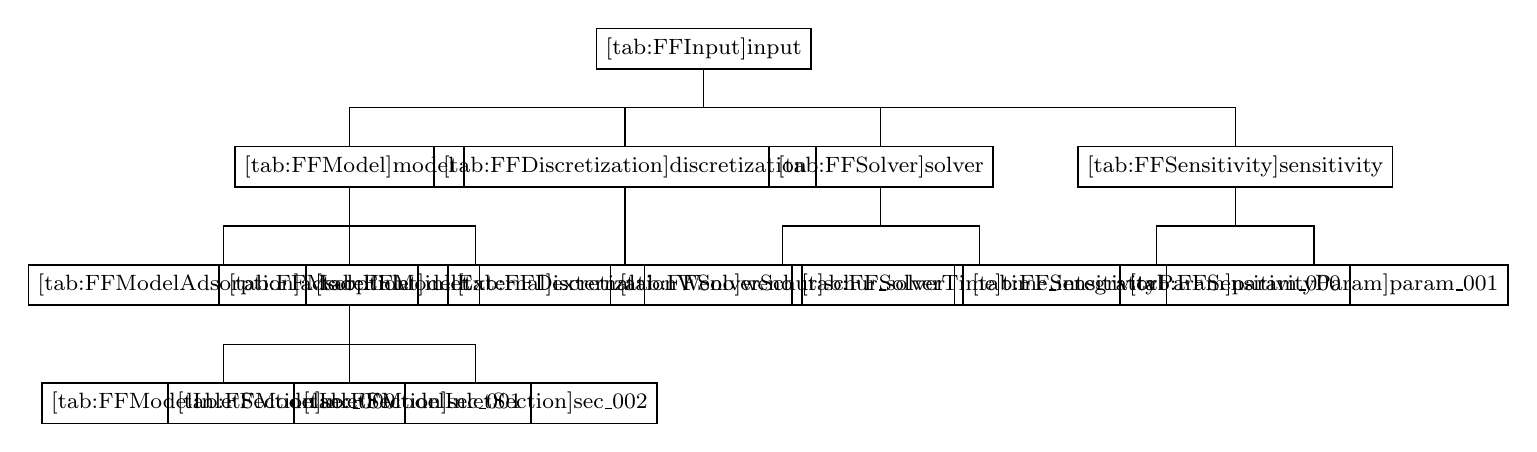
\begin{tikzpicture}[%
  every node/.style={draw=black,semithick,font=\footnotesize},
  level 2/.style={sibling distance=16mm},
  ]
  \node {\hyperref[tab:FFInput]{input}} [edge from parent fork down]
    child[sibling distance=30mm] { node {\hyperref[tab:FFModel]{model} } [edge from parent fork down]
              child { node { \hyperref[tab:FFModelAdsorption]{adsorption} } }
              child { node { \hyperref[tab:FFModelInlet]{inlet} } [edge from parent fork down]
                        child { node { \hyperref[tab:FFModelInletSection]{sec\_000} } }
                        child { node { \hyperref[tab:FFModelInletSection]{sec\_001} } }
                        child { node { \hyperref[tab:FFModelInletSection]{sec\_002} } }
                    }
              child { node { \hyperref[tab:FFModelExternal]{external} } }
          }   
    child[sibling distance=20mm] { node { \hyperref[tab:FFDiscretization]{discretization} } [edge from parent fork down]
              child { node { \hyperref[tab:FFDiscretizationWeno]{weno} } }
          }
    child[sibling distance=45mm] { node { \hyperref[tab:FFSolver]{solver} } [edge from parent fork down]
              child[sibling distance=25mm] { node { \hyperref[tab:FFSolverSchur]{schur\_solver} } }
              child[sibling distance=25mm] { node { \hyperref[tab:FFSolverTime]{time\_integrator} } }
          }
    child[sibling distance=45mm] { node { \hyperref[tab:FFSensitivity]{sensitivity} } [edge from parent fork down]
              child[sibling distance=20mm] { node { \hyperref[tab:FFSensitivityParam]{param\_000} } }
              child[sibling distance=20mm] { node { \hyperref[tab:FFSensitivityParam]{param\_001} } }
          };
\end{tikzpicture}
\caption{\label{fig:FFInput}Structure of the groups in the input part of the file format}
\end{figure}

\begin{figure}[!ht]
\centering
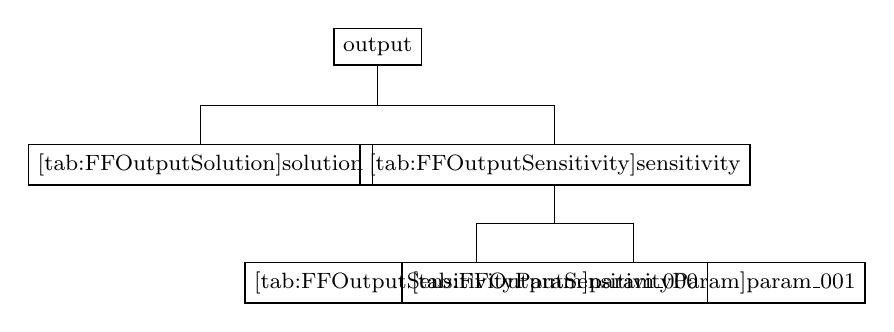
\begin{tikzpicture}[%
  every node/.style={draw=black,semithick,font=\footnotesize},
  ]
  \node {output} [edge from parent fork down]
    child[sibling distance=45mm] { node { \hyperref[tab:FFOutputSolution]{solution} } }   
    child[sibling distance=45mm] { node { \hyperref[tab:FFOutputSensitivity]{sensitivity} } [edge from parent fork down]
              child[sibling distance=20mm] { node { \hyperref[tab:FFOutputSensitivityParam]{param\_000} } }
              child[sibling distance=20mm] { node { \hyperref[tab:FFOutputSensitivityParam]{param\_001} } }
          };
\end{tikzpicture}
\caption{\label{fig:FFOutput}Structure of the groups in the output part of the file format}
\end{figure}

\subsection{Description of datasets}

Reference volumes are denoted by subscripts:
\begin{itemize}
  \item[\si{\cubic\metre\of{Int}}] Interstitial volume
  \item[\si{\cubic\metre\of{MP}}] Bead mobile phase volume
  \item[\si{\cubic\metre\of{SP}}] Bead solid phase volume
\end{itemize}

\newpage

\newcommand{\GroupHeadline}[1]{\small\textbf{Group} \texttt{#1}}

\begin{table}[!ht]
\footnotesize
\begin{tabu}to \linewidth[m]{lXcc} \toprule
\multicolumn{4}{c}{\GroupHeadline{/input}} \\
\rowfont[c]\normalfont Dataset & Description & Type & Range \everyrow{\midrule}\\
\texttt{CHROMATOGRAPHY\_TYPE} & Specifies the type of mass transport model & string &
      \texttt{GENERAL\_RATE\_MODEL} \everyrow{}\\
\bottomrule
\end{tabu}
\caption{\label{tab:FFInput}Datasets in the \texttt{/input} group}
\end{table}

\begin{table}[!ht]
\footnotesize
\begin{tabu}to \linewidth[m]{lX[m]cccc} \toprule
\multicolumn{6}{c}{\GroupHeadline{/input/model}} \\
\rowfont[c]\normalfont Dataset & Description & Unit & Type & Range & Length \everyrow{\midrule}\\
\texttt{NCOMP}& Number of chemical components in the chromatographic media & -- & int  & $\geq 1$ & 1 \\
\texttt{ADSORPTION\_TYPE} & Specifies the type of adsorption model & -- & string & See Table~\ref{tab:FFModelAdsorption} & 1 \\
\texttt{INIT\_C} & A vector with initial concentrations for each comp.\ in the mobile phase & \si{\mol\per\cubic\metre\of{Int \& MP}} & double & $\geq 0.0$ & \texttt{NCOMP}\\
\texttt{INIT\_Q} & Same as \texttt{INIT\_C} but for the bound phase & \si{\mol\per\cubic\metre\of{SP}} & double & $\geq 0.0$ & \texttt{NCOMP}\\
\texttt{COL\_DISPERSION} & Axial dispersion coefficient & \si{\square\metre\of{Int}\per\second} & double & $\geq 0.0$ & 1 / \texttt{NSEC}\\
\texttt{COL\_LENGTH} & Column length & \si{\metre} & double & $> 0.0$ & 1\\
\texttt{COL\_POROSITY} & Column porosity & -- & double & $\geq 0.0$ & 1\\
\texttt{FILM\_DIFFUSION} & A vector with film diffusion coefficients & \si{\metre\per\second} & double & $\geq 0.0$ & \texttt{NCOMP} / {$\texttt{NCOMP} \times \texttt{NSEC}$}\\
\texttt{PAR\_DIFFUSION} & A vector with particle diffusion coefficients & \si{\square\metre\of{MP}\per\second} & double & $\geq 0.0$ & \texttt{NCOMP} / {$\texttt{NCOMP} \times \texttt{NSEC}$}\\
\texttt{PAR\_POROSITY} & Particle porosity & -- & double & $> 0.0$ & 1\\
\texttt{PAR\_RADIUS} & Particle radius & \si{\metre} & double & $> 0.0$ & 1\\
\texttt{PAR\_SURFDIFFUSION} & A vector with particle surface diffusion coefficients & \si{\square\metre\of{SP}\per\second} & double & $\geq 0.0$ & \texttt{NCOMP} / {$\texttt{NCOMP} \times \texttt{NSEC}$}\\
\texttt{VELOCITY} & Interstitial velocity of the mobile phase & \si{\metre\per\second} & double & $> 0.0$ & 1 / \texttt{NSEC}\everyrow{}\\
\bottomrule
\end{tabu}
\caption{\label{tab:FFModel}Datasets in the \texttt{/input/model} group}
\end{table}

\begin{footnotesize}
\tabulinesep=3pt
\begin{longtabu}to \linewidth[m]{l>{\scriptsize}X[m]cccc} \toprule
\multicolumn{6}{c}{\GroupHeadline{/input/model/adsorption}} \\
\rowfont[c]\normalfont Dataset & \normalsize Description & Unit & Type & Range & Length\\
\endfirsthead
%
\toprule
\multicolumn{6}{c}{\GroupHeadline{/input/model/adsorption} Continued} \\
\rowfont[c]\normalfont Dataset & \normalsize Description & Unit & Type & Range & Length\\
\midrule
\endhead
%
\bottomrule
\endfoot
%
\bottomrule
\caption{\label{tab:FFModelAdsorption}Datasets in the \texttt{/input/model/adsorption} group}\\
\endlastfoot
%\multicolumn{5}{c}{\texttt{/input/model/adsorption}} \\
%\rowfont[c]\normalfont Dataset & Description & Unit & Type & Range\\
\midrule
\texttt{IS\_KINETIC} & Selects kinetic or stationary adsorbance mode: 1 = kinetic, 0 = stationary & -- & int & 0/1 & 1\\
\midrule
\multicolumn{6}{l}{If \texttt{ADSORPTION\_MODEL} = \texttt{LINEAR}:} \\ % Top level heading
\midrule
\texttt{LIN\_KA} & A vector with adsorption rate constants in the linear binding model & \si{\cubic\metre\of{MP}\per\cubic\metre\of{SP}\per\second} & double & $\geq 0.0$ & \texttt{NCOMP}\\
\midrule
\texttt{LIN\_KD} & A vector with desorption rate constants in the linear binding model & \si{\per\second} & double & $\geq 0.0$ & \texttt{NCOMP}\\
\midrule
\multicolumn{6}{l}{If \texttt{ADSORPTION\_MODEL} = \texttt{MULTI\_COMPONENT\_LANGMUIR}:} \\ % Top level heading
\midrule
\texttt{MCL\_KA} & A vector with adsorption rate constants in the multi component langmuir model & \si{\cubic\metre\of{MP}\per\mol\per\second} & double & $\geq 0.0$ & \texttt{NCOMP}\\
\midrule
\texttt{MCL\_KD} & A vector with desorption rate constants in the multi component langmuir model & \si{\per\second} & double & $\geq 0.0$ & \texttt{NCOMP}\\
\midrule
\texttt{MCL\_QMAX} & A vector with maximum adsorption capacities in the multi component langmuir model & \si{\mol\per\cubic\metre\of{SP}} & double & $> 0.0$ & \texttt{NCOMP}\\
\midrule
\multicolumn{6}{l}{If \texttt{ADSORPTION\_MODEL} = \texttt{MOBILE\_PHASE\_MODULATORS}:} \\ % Top level heading
\midrule
\texttt{MPM\_KA} & A vector with adsorption rate constants in the mobile phase modulator model & \si{\cubic\metre\of{MP}\per\mol\per\second} & double & $\geq 0.0$ & \texttt{NCOMP}\\
\midrule
\texttt{MPM\_KD} & A vector with desorption rate constants in the mobile phase modulator model & \si{\raiseto{3\beta}\metre\of{MP}\per\raiseto{\beta}\mol\per\second} & double & $\geq 0.0$ & \texttt{NCOMP}\\
\midrule
\texttt{MPM\_QMAX} & A vector with maximum adsorption capacities in the mobile phase modulator model & \si{\mol\per\cubic\metre\of{SP}} & double & $\geq 0.0$ & \texttt{NCOMP}\\
\midrule
\texttt{MPM\_BETA} & A vector with parameters describing the ion-exchange characteristics (IEX) & -- & double & $\geq 0.0$ & \texttt{NCOMP}\\
\midrule
\texttt{MPM\_GAMMA} & A vector with parameters describing the hydrophobicity (HIC) & \si{\cubic\metre\of{MP}\per\mol} & double & $\geq 0.0$ & \texttt{NCOMP}\\
\midrule
\multicolumn{6}{l}{If \texttt{ADSORPTION\_MODEL} = \texttt{EXTERNAL\_LANGMUIR}:} \\ % Top level heading
\midrule
\begin{tabular}{c}
  \texttt{EXTL\_KA} \\
  \texttt{EXTL\_KA\_T} \\
  \texttt{EXTL\_KA\_TT} \\
  \texttt{EXTL\_KA\_TTT} \\
\end{tabular} & All vectors with adsorption rate constant coefficients in the External Function Langmuir model & \begin{tabular}{c}
  \si{\cubic\metre\of{MP}\per\mol\per\second} \\
  \si{\cubic\metre\of{MP}\per\mol\per\second\per\ExternalUnit} \\
  \si{\cubic\metre\of{MP}\per\mol\per\second\per\raiseto{2}\ExternalUnit} \\
  \si{\cubic\metre\of{MP}\per\mol\per\second\per\raiseto{3}\ExternalUnit} \\
\end{tabular} & double & $-\infty - \infty$ & \texttt{NCOMP}\\
\midrule
\begin{tabular}{c}
  \texttt{EXTL\_KD} \\
  \texttt{EXTL\_KD\_T} \\
  \texttt{EXTL\_KD\_TT} \\
  \texttt{EXTL\_KD\_TTT} \\
\end{tabular} & All vectors with desorption rate constant coefficients in the External Function Langmuir model & \begin{tabular}{c}
  \si{\per\second} \\
  \si{\per\second\per\ExternalUnit} \\
  \si{\per\second\per\raiseto{2}\ExternalUnit} \\
  \si{\per\second\per\raiseto{3}\ExternalUnit} \\
\end{tabular} & double & $-\infty - \infty$ & \texttt{NCOMP}\\
\midrule
\begin{tabular}{c}
  \texttt{EXTL\_QMAX} \\
  \texttt{EXTL\_QMAX\_T} \\
  \texttt{EXTL\_QMAX\_TT} \\
  \texttt{EXTL\_QMAX\_TTT} \\
\end{tabular} & All vectors with maximum adsorption capacity coefficients in the External Function Langmuir model & \begin{tabular}{c}
  \si{\mol\per\cubic\metre\of{SP}} \\
  \si{\mol\per\cubic\metre\of{SP}\per\ExternalUnit} \\
  \si{\mol\per\cubic\metre\of{SP}\per\raiseto{2}\ExternalUnit} \\
  \si{\mol\per\cubic\metre\of{SP}\per\raiseto{3}\ExternalUnit} \\
\end{tabular} & double & $-\infty - \infty$ & \texttt{NCOMP}\\
\midrule
\multicolumn{6}{l}{If \texttt{ADSORPTION\_MODEL} = \texttt{STERIC\_MASS\_ACTION}:} \\ % Top level heading
\midrule
\texttt{SMA\_LAMBDA} & Stationary phase capacity (monovalent salt counterions); The total number of binding sites available on the resin surface & \si{\mol\per\cubic\metre\of{SP}} & double & $\geq 0.0$ & 1\\
\midrule
\texttt{SMA\_KA} & A vector with adsorption rate constants in the steric mass action model & \si{\raiseto{3(\nu_i-1)}\metre\of{SP}\raiseto{3}\metre\of{MP}\per\raiseto{\nu_i}\mol\per\second} & double & $\geq 0.0$ & \texttt{NCOMP}\\
\midrule
\texttt{SMA\_KD} & A vector with desorption rate constants in the steric mass action model & \si{\raiseto{3\nu_i}\metre\of{MP}\per\raiseto{\nu_i}\mol\per\second} & double & $\geq 0.0$ & \texttt{NCOMP}\\
\midrule
\texttt{SMA\_NU} & A vector with characteristic charges of the protein; The number of sites $\nu$ that the protein interacts with on the resin surface & -- & double & $\geq 0.0$ & \texttt{NCOMP}\\
\midrule
\texttt{SMA\_SIGMA} & A vector with steric factors of the protein; The number of sites $\sigma$ on the surface that are shielded by the protein and prevented from exchange with the salt counterions in solution & -- & double & $\geq 0.0$ & \texttt{NCOMP}\\
\midrule
\multicolumn{6}{l}{If \texttt{ADSORPTION\_MODEL} = \texttt{SELF\_ASSOCIATION}:} \\ % Top level heading
\midrule
\texttt{SAI\_LAMBDA} & Stationary phase capacity (monovalent salt counterions); The total number of binding sites available on the resin surface & \si{\mol\per\cubic\metre\of{SP}} & double & $\geq 0.0$ & 1\\
\midrule
\texttt{SAI\_KA1} & A vector with adsorption rate constants in the self association model & \si{\raiseto{3(\nu_i-1)}\metre\of{SP}\raiseto{3}\metre\of{MP}\per\raiseto{\nu_i}\mol\per\second} & double & $\geq 0.0$ & \texttt{NCOMP}\\
\midrule
\texttt{SAI\_KA2} & A vector with adsorption rate constants of dimerization in the self association model & \si{\raiseto{3(\nu_i-1)}\metre\of{SP}\raiseto{6}\metre\of{MP}\per\raiseto{(\nu_i+1)}\mol\per\second}  & double & $\geq 0.0$ & \texttt{NCOMP}\\
\midrule
\texttt{SAI\_KD} & A vector with desorption rate constants in the self association model & \si{\raiseto{3\nu_i}\metre\of{MP}\per\raiseto{\nu_i}\mol\per\second} & double & $\geq 0.0$ & \texttt{NCOMP}\\
\midrule
\texttt{SAI\_NU} & A vector with characteristic charges $\nu$ of the protein & -- & double & $\geq 0.0$ & \texttt{NCOMP}\\
\midrule
\texttt{SAI\_SIGMA} & A vector with steric factors $\sigma$ of the protein & -- & double & $\geq 0.0$ & \texttt{NCOMP}\\
\midrule
\multicolumn{6}{l}{If \texttt{ADSORPTION\_MODEL} = \texttt{EXTERNAL\_STERIC\_MASS\_ACTION}:} \\ % Top level heading
\midrule
\begin{tabular}{@{}l@{}}
  \texttt{EXTSMA\_KA} \\
  \texttt{EXTSMA\_KA\_T} \\
  \texttt{EXTSMA\_KA\_TT} \\
  \texttt{EXTSMA\_KA\_TTT} \\
\end{tabular} & All vectors with adsorption rate constants in the thermal steric mass action model & \begin{tabular}{@{}l@{}}
  \si{\raiseto{3(\nu_i-1)}\metre\of{SP}\raiseto{3}\metre\of{MP}\per\raiseto{\nu_i}\mol\per\second} \\
  \si{\raiseto{3(\nu_i-1)}\metre\of{SP}\raiseto{3}\metre\of{MP}\per\raiseto{\nu_i}\mol\per\second\per\ExternalUnit} \\
  \si{\raiseto{3(\nu_i-1)}\metre\of{SP}\raiseto{3}\metre\of{MP}\per\raiseto{\nu_i}\mol\per\second\per\raiseto{2}\ExternalUnit} \\
  \si{\raiseto{3(\nu_i-1)}\metre\of{SP}\raiseto{3}\metre\of{MP}\per\raiseto{\nu_i}\mol\per\second\per\raiseto{3}\ExternalUnit} \\
\end{tabular} & double & $-\infty - \infty$ & \texttt{NCOMP}\\
\midrule 
\begin{tabular}{@{}l@{}}
  \texttt{EXTSMA\_KD} \\
  \texttt{EXTSMA\_KD\_T} \\
  \texttt{EXTSMA\_KD\_TT} \\
  \texttt{EXTSMA\_KD\_TTT} \\
\end{tabular} & All vectors with desorption rate constant coefficients in the thermal steric mass action model & \begin{tabular}{@{}l@{}}
  \si{\raiseto{3\nu_i}\metre\of{MP}\per\raiseto{\nu_i}\mol\per\second} \\
  \si{\raiseto{3\nu_i}\metre\of{MP}\per\raiseto{\nu_i}\mol\per\second\per\ExternalUnit} \\
  \si{\raiseto{3\nu_i}\metre\of{MP}\per\raiseto{\nu_i}\mol\per\second\per\raiseto{2}\ExternalUnit} \\
  \si{\raiseto{3\nu_i}\metre\of{MP}\per\raiseto{\nu_i}\mol\per\second\per\raiseto{3}\ExternalUnit} \\
\end{tabular} & double & $-\infty - \infty$ & \texttt{NCOMP}\\
\midrule
\begin{tabular}{@{}l@{}}
  \texttt{EXTSMA\_NU} \\
  \texttt{EXTSMA\_NU\_T} \\
  \texttt{EXTSMA\_NU\_TT} \\
  \texttt{EXTSMA\_NU\_TTT} \\
\end{tabular} & All vectors with characteristic charges of the protein in the thermal steric mass action model & \begin{tabular}{@{}l@{}}
  --\\
  \si{\per\ExternalUnit} \\
  \si{\per\raiseto{2}\ExternalUnit} \\
  \si{\per\raiseto{3}\ExternalUnit} \\
\end{tabular} & double & $-\infty - \infty$ & \texttt{NCOMP}\\
\midrule
\begin{tabular}{@{}l@{}}
  \texttt{EXTSMA\_SIGMA} \\
  \texttt{EXTSMA\_SIGMA\_T} \\
  \texttt{EXTSMA\_SIGMA\_TT} \\
  \texttt{EXTSMA\_SIGMA\_TTT} \\
\end{tabular} & All vectors with steric factors of the protein in the thermal steric mass action model & \begin{tabular}{@{}l@{}}
  --\\
  \si{\per\ExternalUnit} \\
  \si{\per\raiseto{2}\ExternalUnit} \\
  \si{\per\raiseto{3}\ExternalUnit} \\
\end{tabular} & double & $-\infty - \infty$ & \texttt{NCOMP}\\
\midrule
\begin{tabular}{@{}l@{}}
  \texttt{EXTSMA\_LAMBDA} \\
  \texttt{EXTSMA\_LAMBDA\_T} \\
  \texttt{EXTSMA\_LAMBDA\_TT} \\
  \texttt{EXTSMA\_LAMBDA\_TTT} \\
\end{tabular} & Stationary phase capacity (monovalent salt counterions) in the thermal steric mass action model & \begin{tabular}{@{}l@{}}
  \si{\mol\per\cubic\metre\of{SP}}\\
  \si{\mol\per\cubic\metre\of{SP}\per\ExternalUnit} \\
  \si{\mol\per\cubic\metre\of{SP}\per\raiseto{2}\ExternalUnit} \\
  \si{\mol\per\cubic\metre\of{SP}\per\raiseto{3}\ExternalUnit} \\
\end{tabular} & double & $-\infty - \infty$ & 1\\
\midrule
\multicolumn{6}{l}{If \texttt{ADSORPTION\_MODEL} = \texttt{MULTI\_COMPONENT\_BILANGMUIR}:} \\ % Top level heading
\midrule
\texttt{MCBL\_KA1} & A vector with adsorption rate constants of the first binding site type in the multi component Bi-Langmuir model & \si{\cubic\metre\of{MP}\per\mol\per\second} & double & $\geq 0.0$ & \texttt{NCOMP} / 2 \\
\midrule
\texttt{MCBL\_KA2} & A vector with adsorption rate constants of the second binding site type in the multi component Bi-Langmuir model & \si{\cubic\metre\of{MP}\per\mol\per\second} & double & $\geq 0.0$ & \texttt{NCOMP} / 2 \\
\midrule
\texttt{MCBL\_KD1} & A vector with desorption rate constants of the first binding site type in the multi component Bi-Langmuir model & \si{\per\second} & double & $\geq 0.0$ & \texttt{NCOMP} / 2\\
\midrule
\texttt{MCBL\_KD2} & A vector with desorption rate constants of the second binding site type in the multi component Bi-Langmuir model & \si{\per\second} & double & $\geq 0.0$ & \texttt{NCOMP} / 2\\
\midrule
\texttt{MCBL\_QMAX1} & A vector with with maximum adsorption capacities of the first binding site type & \si{\mol\per\cubic\metre\of{SP}} & double & $> 0.0$ & \texttt{NCOMP} / 2\\
\midrule
\texttt{MCBL\_QMAX2} & A vector with with maximum adsorption capacities of the second binding site type & \si{\mol\per\cubic\metre\of{SP}} & double & $> 0.0$ & \texttt{NCOMP} / 2 \everyrow{}\\
\end{longtabu}
\end{footnotesize}


\begin{table}[!ht]
\footnotesize
\begin{tabu}to \linewidth[m]{lX[m]cccc} \toprule
\multicolumn{6}{c}{\GroupHeadline{/input/model/inlet}} \\
\rowfont[c]\normalfont Dataset & Description & Unit & Type & Range & Length \everyrow{\midrule}\\
\texttt{NSEC} & Number of sections & -- & int & $\geq 1$ & 1\\
\texttt{SECTION\_TIMES} & A vector with simulation times at which inlet function is discontinous; including start and end times & \si{\second} & double & $\geq 0.0$ & \texttt{NSEC}+1\\
\texttt{SECTION\_CONTINUITY} & A vector indicating continuity of each section transition & -- & int &  
  \begin{tabular}{c}
    0 (discontinuous) \\
    1 (continuous)
  \end{tabular} & \texttt{NSEC}-1
\everyrow{}\\
\bottomrule
\end{tabu}
\caption{\label{tab:FFModelInlet}Datasets in the \texttt{/input/model/inlet} group}
\end{table}


\begin{table}[!ht]
\footnotesize
\begin{tabu}to \linewidth[m]{lX[m]cccc} \toprule
\multicolumn{6}{c}{\GroupHeadline{/input/model/inlet/sec\_XXX}} \\
\rowfont[c]\normalfont Dataset & Description & Unit & Type & Range & Length \everyrow{\midrule}\\
\texttt{CONST\_COEFF} & A vector with constant coefficients for inlet concentrations & \si{\mol\per\cubic\metre\of{Int}} & double & $-\infty - \infty$ & \texttt{NCOMP} \\
\texttt{LIN\_COEFF} & A vector with linear coefficients for inlet concentrations & \si{\mol\per\cubic\metre\of{Int}\per\second} & double & $-\infty - \infty$ & \texttt{NCOMP} \\
\texttt{QUAD\_COEFF} & A vector with quadratic coefficients for inlet concentrations & \si{\mol\per\cubic\metre\of{Int}\per\square\second} & double & $-\infty - \infty$ & \texttt{NCOMP} \\
\texttt{CUBE\_COEFF} & A vector with cubic coefficients for inlet concentrations & \si{\mol\per\cubic\metre\of{Int}\per\cubic\second} & double & $-\infty - \infty$ & \texttt{NCOMP} 
\everyrow{}\\
\bottomrule
\end{tabu}
\caption{\label{tab:FFModelInletSection}Datasets in the \texttt{/input/model/inlet/sec\_XXX} groups}
\end{table}


\begin{table}[!ht]
\footnotesize
\begin{tabu}to \linewidth[m]{lX[m]cccc} \toprule
\multicolumn{6}{c}{\GroupHeadline{/input/model/external}} \\
\rowfont[c]\normalfont Dataset & Description & Unit & Type & Range & Length \everyrow{\midrule}\\
\texttt{EXT\_VELOCITY} & Velocity of the external profile in positive column axial direction & \si{\metre\per\second} & double & $-\infty - \infty$ & 1\\
\texttt{EXT\_PROFILE} & A vector with external measurements $T$ & \si{\ExternalUnit} & double & $\geq 0$ & Arbitrary\\
\texttt{EXT\_PROF\_DELTA} & A vector with distances of the external measurements (first entry must be $0.0$) & \si{\metre} & double & $\geq 0.0$ & Same as \texttt{EXT\_PROFILE}
\everyrow{}\\
\bottomrule
\end{tabu}
\caption{\label{tab:FFModelExternal}Datasets in the \texttt{/input/model/external} group}
\end{table}


\begin{table}[!ht]
\footnotesize
\begin{tabu}to \linewidth[m]{lX[m]cccc} \toprule
\multicolumn{6}{c}{\GroupHeadline{/input/discretization}} \\
\rowfont[c]\normalfont Dataset & Description & Unit & Type & Range & Length \everyrow{\midrule}\\
\texttt{NCOL} & Number of column (axial) discretization cells & -- & int & $\geq 1$ & 1\\
\texttt{NPAR} & Number of particle (radial) discretization cells & -- & int & $\geq 1$ & 1\\
\texttt{PAR\_DISC\_TYPE} & Specifies the discretization scheme inside the particles & -- & string
& \begin{tabular}{c}
  \texttt{EQUIDISTANT\_PAR} \\
  \texttt{EQUIVOLUME\_PAR} \\
  \texttt{USER\_DEFINED\_PAR} \\
  \end{tabular} & 1\\
\texttt{PAR\_DISC\_VECTOR} & A vector with node coordinates for the cell boundaries & \si{\metre} & double
  & $0.0-1.0$ & \texttt{NPAR}+1 \\
\texttt{RECONSTRUCTION} & Type of reconstruction method for fluxes & -- & string
& \begin{tabular}{c}
  \texttt{WENO}
  \end{tabular} & 1\everyrow{}\\
\bottomrule
\end{tabu}
\caption{\label{tab:FFDiscretization}Datasets in the \texttt{/input/discretization} group}
\end{table}


\begin{table}[!ht]
\footnotesize
\begin{tabu}to \linewidth[m]{lX[m]cc} \toprule
\multicolumn{4}{c}{\GroupHeadline{/input/discretization/weno}} \\
\rowfont[c]\normalfont Dataset & Description & Type & Range \everyrow{\midrule}\\
\texttt{BOUNDARY\_MODEL} & Boundary model type: 0 = Lower WENO order (stable), 1 = Zero weights (unstable for small $D_{ax}$), 2 = Zero weights for p $\neq$ 0 (stable?), 3 = Large ghost points & int & $0-3$\\
\texttt{WENO\_EPS} & WENO $\varepsilon$ & double & $\geq 0.0$\\
\texttt{WENO\_ORDER} & WENO Order: 1 = standard upwind scheme, 2, 3; also called WENO K & int & $1-3$ \everyrow{}\\
\bottomrule
\end{tabu}
\caption{\label{tab:FFDiscretizationWeno}Datasets in the \texttt{/input/discretization/weno} group}
\end{table}


\begin{table}[!ht]
\footnotesize
\begin{tabu}to \linewidth[m]{lX[m]ccc} \toprule
\multicolumn{5}{c}{\GroupHeadline{/input/solver}} \\
\rowfont[c]\normalfont Dataset & Description & Unit & Type & Range \everyrow{\midrule}\\      
\texttt{NTHREADS} & Number of used OpenMP threads & -- & int & $\geq 1$ \\
\texttt{LOG\_LEVEL} & Specifies the verbosity of the logging output (Only errors;
warning and errors; info and warnings and errors, etc.) & -- & string &
\begin{tabular}{@{}c@{}} \texttt{ERROR} \\
  \texttt{WARNING} \\
  \texttt{INFO} \\
  \texttt{DEBUG1} \\
  \texttt{DEBUG2} \\
  \texttt{TRACE1} \\
  \texttt{TRACE2} \\
\end{tabular} \\
\texttt{PRINT\_CONFIG} & Print configuration message before simulation & -- & int & 0/1 \\
\texttt{PRINT\_PARAMLIST} & Print list of parameters before simulation & -- & int & 0/1 \\
\texttt{PRINT\_PROGRESS} & Print current state of simulation & -- & int & 0/1 \\
\texttt{PRINT\_STATISTICS} & Print integrator statistics after each section & -- & int & 0/1 \\
\texttt{PRINT\_TIMING} & Print timing information after simulation & -- & int & 0/1 \\
\texttt{USE\_ANALYTIC\_JACOBIAN} & Use analytically computed jacobian matrix (faster) instead of jacobian generated by algorithmic differentiation (slower) & -- & int & 0/1 \\
\texttt{USER\_SOLUTION\_TIMES} & A \emph{vector} with timepoints at which a solution is desired & \si{\second} & double & $\geq 0.0$ \\
\texttt{WRITE\_AT\_USER\_TIMES} & Write solutions at times specified by \texttt{USER\_SOLUTION\_TIMES} (write integration timepoints otherwise) & -- & int & 0/1 \\
\texttt{WRITE\_SOLUTION\_TIMES} & Write times at which a solution was produced & -- & int & 0/1 \\
\texttt{WRITE\_SOLUTION\_COLUMN\_INLET} & Write solutions at column inlet (boundary condition) & -- & int & 0/1 \\
\texttt{WRITE\_SOLUTION\_COLUMN\_OUTLET} & Write solutions at column outlet (chromatograms) & -- & int & 0/1 \\
\texttt{WRITE\_SOLUTION\_ALL} & Write all (intermediate) solutions & -- & int & 0/1 \\
\texttt{WRITE\_SENS\_COLUMN\_OUTLET} & Write sensitivity data at column outlet & -- & int & 0/1 \\
\texttt{WRITE\_SENS\_ALL} & Write all (intermediate) sensitivity data & -- & int & 0/1 \everyrow{}\\
\bottomrule
\end{tabu}
\caption{\label{tab:FFSolver}Datasets in the \texttt{/input/solver} group}
\end{table}


\begin{table}[!ht]
\footnotesize
\begin{tabu}to \linewidth[m]{lX[m]cc} \toprule
\multicolumn{4}{c}{\GroupHeadline{/input/solver/schur\_solver}} \\
\rowfont[c]\normalfont Dataset & Description & Type & Range \everyrow{\midrule}\\      
\texttt{GS\_TYPE} & Type of Gram-Schmidt orthogonalization, see IDAS guide
4.5.7.3, 41f. & int &
\begin{tabular}{c}
  0 (\texttt{CLASSICAL\_GS}) \\
  1 (\texttt{MODIFIED\_GS})
\end{tabular} \\
\texttt{MAX\_KRYLOV} & Defines the size of the iterative linear SPGMR solver (0: \texttt{MAX\_KRYLOV} = \texttt{NCOL}) & int & $0-\texttt{NCOL}$\\
\texttt{MAX\_RESTARTS} & Maximum number of restarts in the GMRES algorithm. If lack of memory isn't an issue, better use a larger Krylov space than restarts & int & $\geq 0$ \\
\texttt{SCHUR\_SAFETY} & Schur safety factor; Influences the tradeof between linear iterations and nonlinear error control; see IDAS guide 2.1, 5 & double & $\geq 0.0$ \everyrow{}\\
\bottomrule
\end{tabu}
\caption{\label{tab:FFSolverSchur}Datasets in the \texttt{/input/solver/schur\_solver} group}
\end{table}


\begin{table}[!ht]
\footnotesize
\begin{tabu}to \linewidth[m]{lX[m]cc} \toprule
\multicolumn{4}{c}{\GroupHeadline{/input/solver/time\_integrator}} \\
\rowfont[c]\normalfont Dataset & Description & Type & Range \everyrow{\midrule}\\      
\texttt{ABSTOL} & Absolute tolerance in the solution of the original system & double & $>0.0$\\
\texttt{RELTOL} & Relative tolerance in the solution of the original system & double & $\geq 0.0$\\
\texttt{INIT\_STEP\_SIZE} & Factor which is multiplied by the section length to get initial integrator stepsize (0.0: IDAS default value), see IDAS guide 4.5, 36f. & double & $0.0-1.0$\\
\texttt{MAX\_STEPS} & Maximum number of timesteps taken by IDAS (0: IDAS default = 500), see IDAS guide 4.5, 36 & int & $\geq 0$ \everyrow{}\\
\bottomrule
\end{tabu}
\caption{\label{tab:FFSolverTime}Datasets in the \texttt{/input/solver/time\_integrator} group}
\end{table}


\begin{table}[!ht]
\footnotesize
\begin{tabu}to \linewidth[m]{lX[m]cc} \toprule
\multicolumn{4}{c}{\GroupHeadline{/input/sensitivity}} \\
\rowfont[c]\normalfont Dataset & Description & Type & Range \everyrow{\midrule}\\      
\texttt{NSENS} & Number of sensitivities to be computed & int & $\geq 0$\\
\texttt{SENS\_METHOD} & Method used for computation of sensitivities; algorithmic differentiation or finite differences of order $1-4$ & string
& \begin{tabular}{@{}c@{}}
  \texttt{ad1} \\
  \texttt{fd1} \\
  \texttt{fd2} \\
  \texttt{fd4} \\
  \end{tabular} \everyrow{}\\
\bottomrule
\end{tabu}
\caption{\label{tab:FFSensitivity}Datasets in the \texttt{/input/sensitivity} group}
\end{table}


\begin{table}[!ht]
\footnotesize
\begin{tabu}to \linewidth[m]{lX[m]cc} \toprule
\multicolumn{4}{c}{\GroupHeadline{/input/sensitivity/param\_XXX}} \\
\rowfont[c]\normalfont Dataset & Description & Type & Range \everyrow{\midrule}\\      
\texttt{SENS\_NAME} & Name of the parameter & string & *\footnote{All parameter names allowed that occur in group \texttt{input\_model} except \texttt{NCOMP}, \texttt{INIT\_C}, \texttt{INIT\_Q}, \texttt{ADSORPTION\_TYPE}, \texttt{adsorption/IS\_KINETIC}, \texttt{inlet/NSEC}, \texttt{inlet/SECTION\_TIMES}, \texttt{inlet/SECTION\_CONTINUITY}, and everything in \texttt{external/}} \\
\texttt{SENS\_COMP} & Component index; only for parameters defined for each component (-1 otherwise) & int & $\geq -1$\\
\texttt{SENS\_SECTION} & Section index; only for inlet parameters (-1 otherwise) & int & $\geq -1$\\
\texttt{SENS\_ABSTOL} & Absolute tolerance used in the computation of the sensitivities. Rule of thumb: \texttt{ABSTOL} / \texttt{PARAM\_VALUE} & double & $\geq 0.0$\\
\texttt{SENS\_FD\_DELTA} & Relative disturbance $\Delta p$ in finite difference sensitivity computations & double & $\geq 0.0$\everyrow{}\\
\bottomrule
\end{tabu}
\caption{\label{tab:FFSensitivityParam}Datasets in the \texttt{/input/sensitivity/param\_XXX} groups}
\end{table}


\begin{table}[!ht]
\footnotesize
\begin{tabu}to \linewidth[m]{lX[m]cc} \toprule
\multicolumn{4}{c}{\GroupHeadline{/output/solution}} \\
\rowfont[c]\normalfont Dataset & Description & Unit & Type \everyrow{\midrule}\\      
\texttt{SOLUTION\_TIMES} & Time points at which the solution is written & \si{\second} & double \\
\texttt{SOLUTION\_COLUMN} & Interstitial solution as $n_{\text{Time}} \times n_{\text{Comp}} \times n_{\text{ColCells}}$ tensor in row-major storage & \si{\mol\per\cubic\metre\of{Int}} & double \\
\texttt{SOLUTION\_PARTICLE} & Solution inside the beads as $n_{\text{Time}} \times n_{\text{ColCells}} \times n_{\text{ParCells}} \times 2 \times n_{\text{Comp}}$ tensor in row-major storage & \si{\mol\per\cubic\metre\of{MP \& SP}} & double \\
\texttt{SOLUTION\_BOUNDARY} & Flux solution as $n_{\text{Time}} \times n_{\text{Comp}} \times n_{\text{ColCells}}$ tensor in row-major storage & \si{\mol\per\square\metre\per\second} & double \\
\texttt{SOLUTION\_COLUMN\_OUTLET\_COMP\_XXX} & Component \texttt{XXX} of the solution at the column outlet & \si{\mol\per\cubic\metre\of{Int}} & double \\
\texttt{SOLUTION\_COLUMN\_INLET\_COMP\_XXX} & Component \texttt{XXX} of the solution at the column inlet & \si{\mol\per\cubic\metre\of{Int}} & double 
\everyrow{}\\
\bottomrule
\end{tabu}
\caption{\label{tab:FFOutputSolution}Datasets in the \texttt{/output/solution} group}
\end{table}


\begin{table}[!ht]
\footnotesize
\begin{tabu}to \linewidth[m]{lX[m]cc} \toprule
\multicolumn{3}{c}{\GroupHeadline{/output/sensitivity}} \\
\rowfont[c]\normalfont Dataset & Description & Type \everyrow{\midrule}\\      
\texttt{SENS\_COLUMN} & Interstitial solution as $n_{\text{Time}} \times n_{\text{Comp}} \times n_{\text{ColCells}} \times n_{\text{Params}}$ tensor in row-major storage & double \\
\texttt{SENS\_PARTICLE} & Solution inside the beads as $n_{\text{Time}} \times n_{\text{ColCells}} \times n_{\text{ParCells}} \times 2 \times n_{\text{Comp}} \times n_{\text{Params}}$ tensor in row-major storage & double \\
\texttt{SENS\_BOUNDARY} & Flux solution as $n_{\text{Time}} \times n_{\text{Comp}} \times n_{\text{ColCells}} \times n_{\text{Params}}$ tensor in row-major storage & double
\everyrow{}\\
\bottomrule
\end{tabu}
\caption{\label{tab:FFOutputSensitivity}Datasets in the \texttt{/output/sensitivity} group}
\end{table}


\begin{table}[!ht]
\footnotesize
\begin{tabu}to \linewidth[m]{lX[m]cc} \toprule
\multicolumn{4}{c}{\GroupHeadline{/output/sensitivity/param\_XXX}} \\
\rowfont[c]\normalfont Dataset & Description & Unit & Type \everyrow{\midrule}\\      
\texttt{SENS\_COLUMN\_OUTLET\_COMP\_YYY} & Sensitivity of component \texttt{YYY} at the column outlet with respect to parameter \texttt{XXX} & \si{\mol\per\cubic\metre\of{Int}\per\ParamUnit} & double
\everyrow{}\\
\bottomrule
\end{tabu}
\caption{\label{tab:FFOutputSensitivityParam}Datasets in the \texttt{/output/sensitivity/param\_XXX} groups}
\end{table}


\FloatBarrier
\subsection{Section dependent model parameters}

Some model parameters (see Table~\ref{tab:FFSectionDependentParams}) can be assigned different values for each section. For example, the velocity the column is operated with could differ in the load, wash, and elution phases.
Section dependency is recognized by specifying the appropriate number of values for the parameters (see Length in Table~\ref{tab:FFModel}). 
If a parameter depends on the component and the section, the ordering is such that the values for the components are listed within each section (i.e., ``component-major''):
For example, in a three component system the ordering is \texttt{comp0sec0}, \texttt{comp1sec0}, \texttt{comp2sec0}, \texttt{comp0sec1}, \texttt{comp1sec1}, \texttt{comp2sec1}, \ldots

Note that single components of component dependent datasets cannot be section dependent.

\begin{table}[!ht]
\centering
\footnotesize
\begin{tabu}to \linewidth[m]{lcc} \toprule
\rowfont[c]\normalfont Dataset & Component dependent & Section dependent \everyrow{\midrule}\\      
\texttt{COL\_DISPERSION} & & \checkmark \\
\texttt{FILM\_DIFFUSION} & \checkmark  & \checkmark \\
\texttt{PAR\_DIFFUSION} & \checkmark  & \checkmark \\
\texttt{PAR\_SURFDIFFUSION} & \checkmark  & \checkmark \\
\texttt{VELOCITY} & & \checkmark \everyrow{}\\
\bottomrule
\end{tabu}
\caption{\label{tab:FFSectionDependentParams}Section dependent datasets in the \texttt{/input/model} group}
\end{table}


% =============================================================================
%  CADET - The Chromatography Analysis and Design Toolkit
%  
%  Copyright © 2008-2015: Eric von Lieres¹, Joel Andersson,
%                         Andreas Puettmann¹, Sebastian Schnittert¹,
%                         Samuel Leweke¹
%                                      
%    ¹ Forschungszentrum Juelich GmbH, IBG-1, Juelich, Germany.
%  
%  All rights reserved. This program and the accompanying materials
%  are made available under the terms of the GNU Public License v3.0 (or, at
%  your option, any later version) which accompanies this distribution, and
%  is available at http://www.gnu.org/licenses/gpl.html
% =============================================================================

\section{Isotherms}

\subsection{Linear}

\begin{align*}
  \frac{\mathrm{d} q_i}{\mathrm{d} t} = k_a c_{p,i} - k_d q_i && \forall i = 1, \dots, N_{\text{comp}}
\end{align*}

\begin{table}[!ht]
  \footnotesize
  \begin{tabu}to \linewidth[m]{lX[m]c}
    \toprule
      \textbf{Constant} & \textbf{Description} & \textbf{Unit} \\
    \midrule
      $k_a$ & Adsorption rate & \si{\cubic\metre\of{MP}\per\cubic\metre\of{SP}\per\second} \\ \midrule
      $k_d$ & Desorption rate & \si{\per\second} \\
    \bottomrule
  \end{tabu}
  \caption{Parameters of the linear adsorption model}
\end{table}

\subsection{Multi Component Langmuir}

\begin{align*}
  \frac{\mathrm{d} q_i}{\mathrm{d} t} = k_a\: c_{p,i}\: q_{\text{max},i} \left( 1 - \sum_{j=1}^{N_{\text{comp}}} \frac{q_j}{q_{\text{max},j}} \right) - k_d q_i && \forall i = 1, \dots, N_{\text{comp}}
\end{align*}

\begin{table}[!ht]
  \footnotesize
  \begin{tabu}to \linewidth[m]{lX[m]c}
    \toprule
      \textbf{Constant} & \textbf{Description} & \textbf{Unit} \\
    \midrule
      $k_a$ & Adsorption rate & \si{\cubic\metre\of{MP}\per\mol\per\second} \\ \midrule
      $k_d$ & Desorption rate & \si{\per\second} \\ \midrule
      $q_{\text{max}}$ & Maximum adsorption capacity; Maximum concentration & \si{\mol\per\cubic\metre\of{SP}} \\
    \bottomrule
  \end{tabu}
  \caption{Parameters of the Multi Component Langmuir adsorption model}
\end{table}

\subsection{Steric Mass Action}

\begin{align*}
  \frac{\mathrm{d} q_i}{\mathrm{d} t} = k_a c_{p,i}\left( \Lambda - \sum_{j=1}^{N_{\text{comp}}} \left( \nu_j + \sigma_j \right) q_j \right)^{\nu_i} - k_d\: q_i\: c_{p,0}^{\nu_i} && \forall i = 1, \dots, N_{\text{comp}}
\end{align*}
where $c_{p,0}$ and $q_0$ denote the salt concentrations in the liquid and solid phase of the beads respectively. A neutrality condition compensating for the missing equation for $\frac{\mathrm{d} q_0}{\mathrm{d}t}$ is required:
\begin{align*}
  q_0 = \Lambda - \sum_{j=1}^{N_{\text{comp}}} \nu_j q_j
\end{align*}

\begin{table}[!ht]
  \footnotesize
  \begin{tabu}to \linewidth[m]{lX[m]c}
    \toprule
      \textbf{Constant} & \textbf{Description} & \textbf{Unit} \\
    \midrule
      $\Lambda$ & Stationary phase capacity (monovalent salt counterions); The total number of binding sites available on the resin surface & \si{\mol\per\cubic\metre\of{SP}} \\ \midrule
      $k_a$ & Adsorption rate & \si{\raiseto{3(\nu_i-1)}\metre\of{SP}\raiseto{3}\metre\of{MP}\per\raiseto{\nu_i}\mol\per\second} \\ \midrule
      $k_d$ & Desorption rate & \si{\raiseto{3\nu_i}\metre\of{MP}\per\raiseto{\nu_i}\mol\per\second} \\ \midrule
      $\nu$ & Characteristic charges of the protein; The number of sites $\nu$ that the protein interacts with on the resin surface & -- \\ \midrule
      $\sigma$ & Steric factors of the protein; The number of sites $\sigma$ on the surface that are shielded by the protein and prevented from exchange with the salt counterions in solution & -- \\
    \bottomrule
  \end{tabu}
  \caption{Parameters of the Steric Mass Action adsorption model}
\end{table}

\subsection{Self Association}

\begin{align*}
  \frac{\mathrm{d} q_i}{\mathrm{d} t} = c_{p,i}\left( \Lambda - \sum_{j=1}^{N_{\text{comp}}} \left( \nu_j + \sigma_j \right) q_j \right)^{\nu_i} \left[ k_{a,1} + k_{a,2} c_{p,i} \right] - k_d\: q_i\: c_{p,0}^{\nu_i} && \forall i = 1, \dots, N_{\text{comp}}
\end{align*}
where $c_{p,0}$ and $q_0$ denote the salt concentrations in the liquid and solid phase of the beads respectively. A neutrality condition compensating for the missing equation for $\frac{\mathrm{d} q_0}{\mathrm{d}t}$ is required:
\begin{align*}
  q_0 = \Lambda - \sum_{j=1}^{N_{\text{comp}}} \nu_j q_j
\end{align*}

\begin{table}[!ht]
  \footnotesize
  \begin{tabu}to \linewidth[m]{lX[m]c}
    \toprule
      \textbf{Constant} & \textbf{Description} & \textbf{Unit} \\
    \midrule
      $\Lambda$ & Stationary phase capacity (monovalent salt counterions); The total number of binding sites available on the resin surface & \si{\mol\per\cubic\metre\of{SP}} \\ \midrule
      $k_{a,1}$ & Adsorption rate & \si{\raiseto{3(\nu_i-1)}\metre\of{SP}\raiseto{3}\metre\of{MP}\per\raiseto{\nu_i}\mol\per\second} \\ \midrule
      $k_{a,2}$ & Adsorption rate of dimerization & \si{\raiseto{3(\nu_i-1)}\metre\of{SP}\raiseto{6}\metre\of{MP}\per\raiseto{(\nu_i+1)}\mol\per\second} \\ \midrule
      $k_d$ & Desorption rate & \si{\raiseto{3\nu_i}\metre\of{MP}\per\raiseto{\nu_i}\mol\per\second} \\ \midrule
      $\nu$ & Characteristic charges of the protein; The number of sites $\nu$ that the protein interacts with on the resin surface & -- \\ \midrule
      $\sigma$ & Steric factors of the protein; The number of sites $\sigma$ on the surface that are shielded by the protein and prevented from exchange with the salt counterions in solution & -- \\
    \bottomrule
  \end{tabu}
  \caption{Parameters of the Self Association adsorption model}
\end{table}

\subsection{Mobile Phase Modulators Langmuir}

\begin{align*}
  \frac{\mathrm{d} q_i}{\mathrm{d} t} = k_a e^{\gamma c_{p,0}} c_{p,i}\: q_{\text{max},i} \left( 1 - \sum_{j=1}^{N_{\text{comp}}} \frac{q_j}{q_{\text{max},j}} \right) - k_d \: c_{p,0}^\beta \: q_i && \forall i = 1, \dots, N_{\text{comp}}
\end{align*}
where $c_{p,0}$ and $q_0$ denote the salt concentrations in the liquid and solid phase of the beads respectively. Salt is considered to be inert, therefore
\begin{align*}
  \frac{\mathrm{d} q_0}{\mathrm{d} t} = 0.
\end{align*}

\begin{table}[!ht]
  \footnotesize
  \begin{tabu}to \linewidth[m]{lX[m]c}
    \toprule
      \textbf{Constant} & \textbf{Description} & \textbf{Unit} \\
    \midrule
      $k_a$ & Adsorption rate & \si{\cubic\metre\of{MP}\per\mol\per\second} \\ \midrule
      $k_d$ & Desorption rate & \si{\raiseto{3\beta}\metre\of{MP}\per\raiseto{\beta}\mol\per\second} \\ \midrule
      $q_{\text{max}}$ & Maximum adsorption capacity; Maximum concentration & \si{\mol\per\cubic\metre\of{SP}} \\ \midrule
      $\gamma$ & Hydrophobicity & \si{\cubic\metre\of{MP}\per\mol} \\ \midrule
      $\beta$ & Describes ion-exchange characteristics & -- \\
    \bottomrule
  \end{tabu}
  \caption{Parameters of the Mobile Phase Modulators Langmuir adsorption model}
\end{table}

\subsection{External Function Multi Component Langmuir}

The same as ordinary Multi Component Langmuir but with coefficients $k_a$, $k_d$, and $q_{\text{max}}$ depending on an external quantity denoted by $T$:
\begin{align*}
  \frac{\mathrm{d} q_i}{\mathrm{d} t} = k_a(T)\: c_{p,i}\: q_{\text{max},i}(T) \left( 1 - \sum_{j=1}^{N_{\text{comp}}} \frac{q_j}{q_{\text{max},j}(T)} \right) - k_d(T) q_i && \forall i = 1, \dots, N_{\text{comp}}
\end{align*}
where the dependence is modeled by a polynomial of third degree, i.e.
\begin{align*}
  k_a(T) &= k_{a,3} T^3 + k_{a,2} T^2 + k_{a,1} T + k_{a,0}, \\
  k_d(T) &= k_{d,3} T^3 + k_{d,2} T^2 + k_{d,1} T + k_{d,0}, \\
  q_{\text{max}}(T) &= q_{\text{max},3} T^3 + q_{\text{max},2} T^2 + q_{\text{max},1} T + q_{\text{max},0}.
\end{align*}
The quantity $T(t, z)$ is a function of time $t$ and space $z$, i.e.\ $T\colon [0, t_{\text{max}}] \times [0, L] \rightarrow \mathds{R}$, which is externally given to the simulator.

\begin{table}[!ht]
  \footnotesize
  \begin{tabu}to \linewidth[m]{lX[m]c}
    \toprule
      \textbf{Constant} & \textbf{Description} & \textbf{Unit} \\
    \midrule
      $k_{a,3}$ & \multirow{4}{*}{Adsorption rate} & \si{\cubic\metre\of{MP}\per\mol\per\second\per\raiseto{3}\ExternalUnit} \\
      $k_{a,2}$ & & \si{\cubic\metre\of{MP}\per\mol\per\second\per\raiseto{2}\ExternalUnit} \\
      $k_{a,1}$ & & \si{\cubic\metre\of{MP}\per\mol\per\second\per\ExternalUnit} \\
      $k_{a,0}$ & & \si{\cubic\metre\of{MP}\per\mol\per\second} \\ \midrule
      $k_{d,3}$ & \multirow{4}{*}{Desorption rate} & \si{\per\second\per\raiseto{3}\ExternalUnit} \\
      $k_{d,2}$ & & \si{\per\second\per\raiseto{2}\ExternalUnit} \\
      $k_{d,1}$ & & \si{\per\second\per\ExternalUnit} \\
      $k_{d,0}$ & & \si{\per\second} \\ \midrule
      $q_{\text{max},3}$ & \multirow{4}{*}{Maximum adsorption capacity; Maximum concentration} & \si{\mol\per\cubic\metre\of{SP}\per\raiseto{3}\ExternalUnit} \\
      $q_{\text{max},2}$ & & \si{\mol\per\cubic\metre\of{SP}\per\raiseto{2}\ExternalUnit} \\
      $q_{\text{max},1}$ & & \si{\mol\per\cubic\metre\of{SP}\per\ExternalUnit} \\
      $q_{\text{max},0}$ & & \si{\mol\per\cubic\metre\of{SP}} \\ \midrule
      $T$ & External quantity & \si{\ExternalUnit} \\ 
    \bottomrule
  \end{tabu}
  \caption{Parameters of the External Function Multi Component Langmuir adsorption model}
\end{table}

\subsection{External Function Steric Mass Action}

The same as ordinary Steric Mass Action but with coefficients $k_a$, $k_d$, $\nu$, $\sigma$ and $\Lambda$ depending on an external quantity denoted by $T$:
\begin{align*}
  \frac{\mathrm{d} q_i}{\mathrm{d} t} &= k_a(T) c_{p,i}\left( \Lambda(T) - \sum_{j=1}^{N_{\text{comp}}} \left( \nu_j(T) + \sigma_j(T) \right) q_j \right)^{\nu_i(T)} - k_d(T)\: q_i\: c_{p,0}^{\nu_i(T)} && \forall i = 1, \dots, N_{\text{comp}} \\
  q_0 &= \Lambda(T) - \sum_{j=1}^{N_{\text{comp}}} \nu_j(T) q_j
\end{align*}
where the dependence is modeled by a polynomial of third degree, i.e.
\begin{align*}
  k_a(T) &= k_{a,3} T^3 + k_{a,2} T^2 + k_{a,1} T + k_{a,0}, \\
  k_d(T) &= k_{d,3} T^3 + k_{d,2} T^2 + k_{d,1} T + k_{d,0}, \\
  \nu(T) &= \nu_3 T^3 + \nu_2 T^2 + \nu_1 T + \nu_0, \\
  \sigma(T) &= \sigma_3 T^3 + \sigma_2 T^2 + \sigma_1 T + \sigma_0, \\
  \Lambda(T) &= \Lambda_3 T^3 + \Lambda_2 T^2 + \Lambda_1 T + \Lambda_0.
\end{align*}
The quantity $T(t, z)$ is a function of time $t$ and space $z$, i.e.\ $T\colon [0, t_{\text{max}}] \times [0, L] \rightarrow \mathds{R}$, which is externally given to the simulator.

\begin{table}[!ht]
  \footnotesize
  \begin{tabu}to \linewidth[m]{lX[m]c}
    \toprule
      \textbf{Constant} & \textbf{Description} & \textbf{Unit} \\
    \midrule
      $k_{a,3}$ & \multirow{4}{*}{Adsorption rate} & \si{\raiseto{3(\nu(T)-1)}\metre\of{SP}\raiseto{3}\metre\of{MP}\per\raiseto{\nu(T)}\mol\per\second\per\raiseto{3}\ExternalUnit} \\
      $k_{a,2}$ & & \si{\raiseto{3(\nu(T)-1)}\metre\of{SP}\raiseto{3}\metre\of{MP}\per\raiseto{\nu(T)}\mol\per\second\per\raiseto{2}\ExternalUnit} \\
      $k_{a,1}$ & & \si{\raiseto{3(\nu(T)-1)}\metre\of{SP}\raiseto{3}\metre\of{MP}\per\raiseto{\nu(T)}\mol\per\second\per\ExternalUnit} \\
      $k_{a,0}$ & & \si{\raiseto{3(\nu(T)-1)}\metre\of{SP}\raiseto{3}\metre\of{MP}\per\raiseto{\nu(T)}\mol\per\second} \\ \midrule
      $k_{d,3}$ & \multirow{4}{*}{Desorption rate} & \si{\raiseto{3\nu(T)}\metre\of{MP}\per\raiseto{\nu(T)}\mol\per\second\per\raiseto{3}\ExternalUnit} \\
      $k_{d,2}$ & & \si{\raiseto{3\nu(T)}\metre\of{MP}\per\raiseto{\nu(T)}\mol\per\second\per\raiseto{2}\ExternalUnit} \\
      $k_{d,1}$ & & \si{\raiseto{3\nu(T)}\metre\of{MP}\per\raiseto{\nu(T)}\mol\per\second\per\ExternalUnit} \\
      $k_{d,0}$ & & \si{\raiseto{3\nu(T)}\metre\of{MP}\per\raiseto{\nu(T)}\mol\per\second} \\ \midrule
      $\Lambda_3$ & \multirow{4}{*}{Stationary phase capacity (monovalent salt counterions)} & \si{\mol\per\cubic\metre\of{SP}\per\raiseto{3}\ExternalUnit} \\
      $\Lambda_2$ & & \si{\mol\per\cubic\metre\of{SP}\per\raiseto{2}\ExternalUnit} \\
      $\Lambda_1$ & & \si{\mol\per\cubic\metre\of{SP}\per\raiseto{1}\ExternalUnit} \\
      $\Lambda_0$ & & \si{\mol\per\cubic\metre\of{SP}} \\ \midrule
      $\nu_3$ & \multirow{4}{*}{Characteristic charges of the protein} & \si{\per\raiseto{3}\ExternalUnit} \\ 
      $\nu_2$ & & \si{\per\raiseto{2}\ExternalUnit} \\ 
      $\nu_1$ & & \si{\per\raiseto{1}\ExternalUnit} \\ 
      $\nu_0$ & & -- \\ \midrule
      $\sigma$ & \multirow{4}{*}{Steric factors of the protein} & \si{\per\raiseto{3}\ExternalUnit} \\
      $\sigma$ & & \si{\per\raiseto{2}\ExternalUnit} \\
      $\sigma$ & & \si{\per\raiseto{1}\ExternalUnit} \\    
      $\sigma$ & & -- \\ \midrule
      $T$ & External quantity & \si{\ExternalUnit} \\ 
    \bottomrule
  \end{tabu}
  \caption{Parameters of the External Function Steric Mass Action adsorption model}
\end{table}

\subsection{External Function Mobile Phase Modulators Langmuir}

The same as ordinary Mobile Phase Modulators Langmuir but with coefficients $k_a, k_d, q_{\text{max}}, \gamma$ and $\beta$ depending on an external quantity denoted by $T$:
\begin{align*}
  \frac{\mathrm{d} q_i}{\mathrm{d} t} = k_a(T) e^{\gamma(T) c_{p,0}} c_{p,i}\: q_{\text{max},i}(T) \left( 1 - \sum_{j=1}^{N_{\text{comp}}} \frac{q_j}{q_{\text{max},j}(T)} \right) - k_d(T) \: c_{p,0}^{\beta(T)} \: q_i && \forall i = 1, \dots, N_{\text{comp}}
\end{align*}
where the dependence is modeled by a polynomial of third degree, i.e.
\begin{align*}
  k_a(T) &= k_{a,3} T^3 + k_{a,2} T^2 + k_{a,1} T + k_{a,0}, \\
  k_d(T) &= k_{d,3} T^3 + k_{d,2} T^2 + k_{d,1} T + k_{d,0}, \\
  q_{\text{max}}(T) &= q_{\text{max},3} T^3 + q_{\text{max},2} T^2 + q_{\text{max},1} T + q_{\text{max},0}, \\
  \gamma(T) &= \gamma_3 T^3 + \gamma_2 T^2 + \gamma_1 T + \gamma_0, \\
  \beta(T) &= \beta_3 T^3 + \beta_2 T^2 + \beta_1 T + \beta_0.
\end{align*}
The quantity $T(t, z)$ is a function of time $t$ and space $z$, i.e.\ $T\colon [0, t_{\text{max}}] \times [0, L] \rightarrow \mathds{R}$, which is externally given to the simulator.

\begin{table}[!ht]
  \footnotesize
  \begin{tabu}to \linewidth[m]{lX[m]c}
    \toprule
      \textbf{Constant} & \textbf{Description} & \textbf{Unit} \\
    \midrule
      $k_{a,3}$ & \multirow{4}{*}{Adsorption rate} & \si{\cubic\metre\of{MP}\per\mol\per\second\per\raiseto{3}\ExternalUnit} \\
      $k_{a,2}$ & & \si{\cubic\metre\of{MP}\per\mol\per\second\per\raiseto{2}\ExternalUnit} \\
      $k_{a,1}$ & & \si{\cubic\metre\of{MP}\per\mol\per\second\per\ExternalUnit} \\
      $k_{a,0}$ & & \si{\cubic\metre\of{MP}\per\mol\per\second} \\ \midrule
      $k_{d,3}$ & \multirow{4}{*}{Desorption rate} & \si{\raiseto{3\beta}\metre\of{MP}\per\raiseto{\beta}\mol\per\second\per\raiseto{3}\ExternalUnit} \\
      $k_{d,2}$ & & \si{\raiseto{3\beta}\metre\of{MP}\per\raiseto{\beta}\mol\per\second\per\raiseto{2}\ExternalUnit} \\
      $k_{d,1}$ & & \si{\raiseto{3\beta}\metre\of{MP}\per\raiseto{\beta}\mol\per\second\per\ExternalUnit} \\
      $k_{d,0}$ & & \si{\raiseto{3\beta}\metre\of{MP}\per\raiseto{\beta}\mol\per\second} \\ \midrule
      $q_{\text{max},3}$ & \multirow{4}{*}{Maximum adsorption capacity; Maximum concentration} & \si{\mol\per\cubic\metre\of{SP}} \\
      $q_{\text{max},2}$ & & \si{\mol\per\cubic\metre\of{SP}\per\raiseto{2}\ExternalUnit} \\
      $q_{\text{max},1}$ & & \si{\mol\per\cubic\metre\of{SP}\per\ExternalUnit} \\
      $q_{\text{max},0}$ & & \si{\mol\per\cubic\metre\of{SP}} \\ \midrule
      $\gamma_3$ & \multirow{4}{*}{Hydrophobicity} & \si{\cubic\metre\of{MP}\per\mol\per\raiseto{3}\ExternalUnit} \\
      $\gamma_2$ & & \si{\cubic\metre\of{MP}\per\mol\per\raiseto{2}\ExternalUnit} \\
      $\gamma_1$ & & \si{\cubic\metre\of{MP}\per\mol\per\ExternalUnit} \\
      $\gamma_0$ & & \si{\cubic\metre\of{MP}\per\mol} \\ \midrule
      $\beta_3$ & \multirow{4}{*}{Describes ion-exchange characteristics} & \si{\per\raiseto{3}\ExternalUnit} \\
      $\beta_2$ & & \si{\per\raiseto{2}\ExternalUnit} \\
      $\beta_1$ & & \si{\per\ExternalUnit} \\
      $\beta_0$ & & -- \\ \midrule
      $T$ & External quantity & \si{\ExternalUnit} \\ 
    \bottomrule
  \end{tabu}
  \caption{Parameters of the External Function Mobile Phase Modulators Langmuir adsorption model}
\end{table}

\subsection{Multi Component Bi-Langmuir}

The Multi Component Bi-Langmuir model adds a second type of binding site $q_i^B$ to the Langmuir model without allowing an exchange between the two sites $q_i^A$ and $q_i^B$.
Therefore, there are no competitivity effects between the two types of binding sites and they have independent capacities.
\begin{align*}
  \frac{\mathrm{d} q_i^A}{\mathrm{d} t} &=  k_a^A\: c_{p,i}\: q_{\text{max},i}^A \left( 1 - \sum_{j=1}^{N_{\text{comp}}} \frac{q_j^A}{q_{\text{max},j}^A}\right) - k_d^A q_i^A & \forall i = 1, \dots, N_{\text{comp}} \\
  \frac{\mathrm{d} q_i^B}{\mathrm{d} t} &=  k_a^B\: c_{p,i}\: q_{\text{max},i}^B \left( 1 - \sum_{j=1}^{N_{\text{comp}}} \frac{q_j^B}{q_{\text{max},j}^B}\right) - k_d^B q_i^B & \forall i = 1, \dots, N_{\text{comp}}
\end{align*}

\begin{table}[!ht]
  \footnotesize
  \begin{tabu}to \linewidth[m]{lX[m]c}
    \toprule
      \textbf{Constant} & \textbf{Description} & \textbf{Unit} \\
    \midrule
      $k_a^A$ & Adsorption rate of first binding site type & \si{\cubic\metre\of{MP}\per\mol\per\second} \\ \midrule
      $k_a^B$ & Adsorption rate of second binding site type & \si{\cubic\metre\of{MP}\per\mol\per\second} \\ \midrule
      $k_d^A$ & Desorption rate of first binding site type & \si{\per\second} \\ \midrule
      $k_d^B$ & Desorption rate of second binding site type & \si{\per\second} \\ \midrule
      $q_{\text{max}}^A$ & Maximum adsorption capacity; Maximum concentration of first binding site type & \si{\mol\per\cubic\metre\of{SP}} \\ \midrule
      $q_{\text{max}}^B$ & Maximum adsorption capacity; Maximum concentration of second binding site type & \si{\mol\per\cubic\metre\of{SP}} \\
    \bottomrule
  \end{tabu}
  \caption{Parameters of the Multi Component Bi-Langmuir adsorption model}
\end{table}


\end{document}
}
	\end{center}
\end{titlepage}

\pagenumbering{Roman}
\tableofcontents

\newpage
\listoffigures

\newpage
\listoftables

\newpage
\pagenumbering{arabic}
\setcounter{page}{1}

% =============================================================================
%  CADET - The Chromatography Analysis and Design Toolkit
%  
%  Copyright © 2008-2014: Eric von Lieres¹, Joel Andersson,
%                         Andreas Puettmann¹, Sebastian Schnittert¹,
%                         Samuel Leweke¹
%                                      
%    ¹ Forschungszentrum Juelich GmbH, IBG-1, Juelich, Germany.
%  
%  All rights reserved. This program and the accompanying materials
%  are made available under the terms of the GNU Public License v3.0 (or, at
%  your option, any later version) which accompanies this distribution, and
%  is available at http://www.gnu.org/licenses/gpl.html
% =============================================================================

\section{CADET File Format Specifications}
The CADET framework is designed to work on a file format structured into groups and datasets. This
concept may be implemented by different file formats.
So far readers and writers for the HDF5 and XML formats have been implemented. The choice is not
limited to those two formats but can be extended as needed.
The layout of such files is described in this section. 

Most of the names of the groups and datasets are predefined in the C++ header file
\texttt{CadetEnumeration.hpp}.
Every valid CADET file needs an \texttt{input} group. It does not need an \texttt{output} group,
since this is created when results are written. If not explicitly stated otherwise, all datasets
are mandatory. By convention all group names are lowercase, whereas all dataset names are uppercase.

\begin{figure}[!ht]
\centering
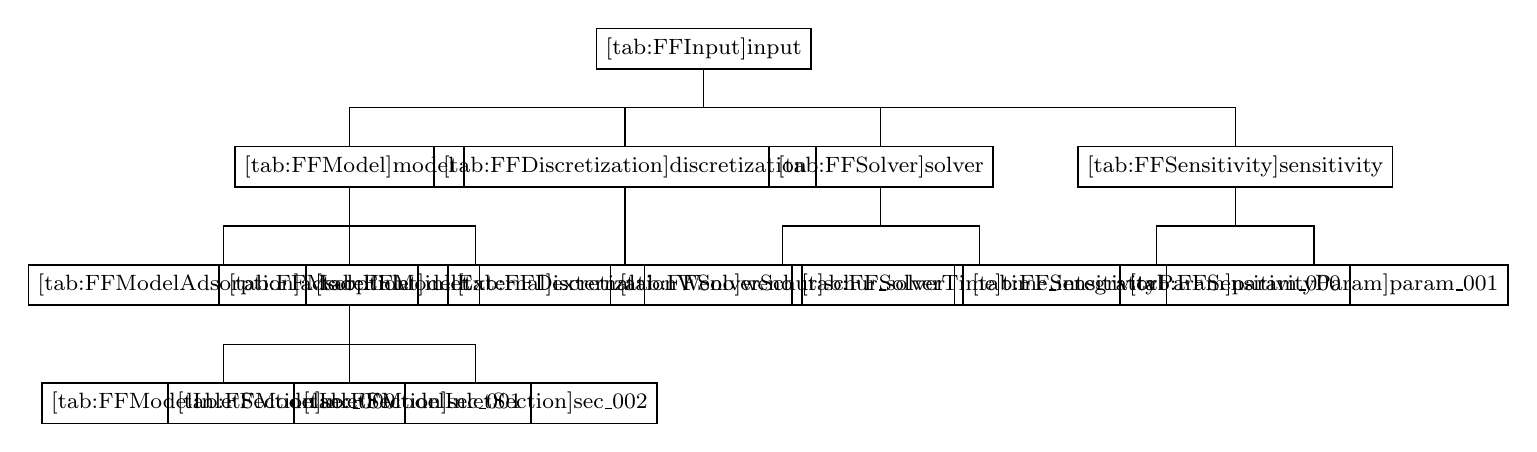
\begin{tikzpicture}[%
  every node/.style={draw=black,semithick,font=\footnotesize},
  level 2/.style={sibling distance=16mm},
  ]
  \node {\hyperref[tab:FFInput]{input}} [edge from parent fork down]
    child[sibling distance=30mm] { node {\hyperref[tab:FFModel]{model} } [edge from parent fork down]
              child { node { \hyperref[tab:FFModelAdsorption]{adsorption} } }
              child { node { \hyperref[tab:FFModelInlet]{inlet} } [edge from parent fork down]
                        child { node { \hyperref[tab:FFModelInletSection]{sec\_000} } }
                        child { node { \hyperref[tab:FFModelInletSection]{sec\_001} } }
                        child { node { \hyperref[tab:FFModelInletSection]{sec\_002} } }
                    }
              child { node { \hyperref[tab:FFModelExternal]{external} } }
          }   
    child[sibling distance=20mm] { node { \hyperref[tab:FFDiscretization]{discretization} } [edge from parent fork down]
              child { node { \hyperref[tab:FFDiscretizationWeno]{weno} } }
          }
    child[sibling distance=45mm] { node { \hyperref[tab:FFSolver]{solver} } [edge from parent fork down]
              child[sibling distance=25mm] { node { \hyperref[tab:FFSolverSchur]{schur\_solver} } }
              child[sibling distance=25mm] { node { \hyperref[tab:FFSolverTime]{time\_integrator} } }
          }
    child[sibling distance=45mm] { node { \hyperref[tab:FFSensitivity]{sensitivity} } [edge from parent fork down]
              child[sibling distance=20mm] { node { \hyperref[tab:FFSensitivityParam]{param\_000} } }
              child[sibling distance=20mm] { node { \hyperref[tab:FFSensitivityParam]{param\_001} } }
          };
\end{tikzpicture}
\caption{\label{fig:FFInput}Structure of the groups in the input part of the file format}
\end{figure}

\begin{figure}[!ht]
\centering
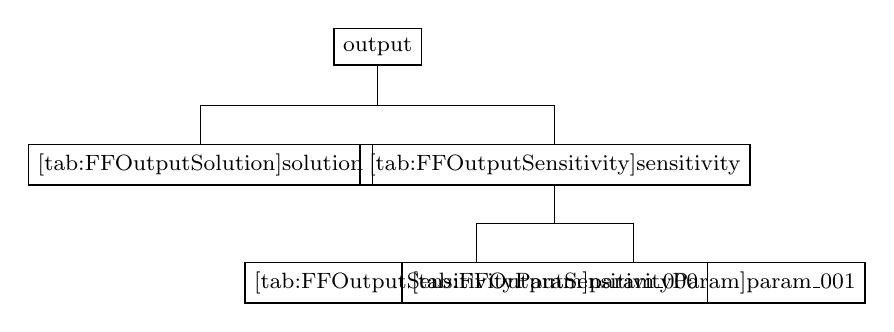
\begin{tikzpicture}[%
  every node/.style={draw=black,semithick,font=\footnotesize},
  ]
  \node {output} [edge from parent fork down]
    child[sibling distance=45mm] { node { \hyperref[tab:FFOutputSolution]{solution} } }   
    child[sibling distance=45mm] { node { \hyperref[tab:FFOutputSensitivity]{sensitivity} } [edge from parent fork down]
              child[sibling distance=20mm] { node { \hyperref[tab:FFOutputSensitivityParam]{param\_000} } }
              child[sibling distance=20mm] { node { \hyperref[tab:FFOutputSensitivityParam]{param\_001} } }
          };
\end{tikzpicture}
\caption{\label{fig:FFOutput}Structure of the groups in the output part of the file format}
\end{figure}

\subsection{Description of datasets}

Reference volumes are denoted by subscripts:
\begin{itemize}
  \item[\si{\cubic\metre\of{Int}}] Interstitial volume
  \item[\si{\cubic\metre\of{MP}}] Bead mobile phase volume
  \item[\si{\cubic\metre\of{SP}}] Bead solid phase volume
\end{itemize}

\newpage

\newcommand{\GroupHeadline}[1]{\small\textbf{Group} \texttt{#1}}

\begin{table}[!ht]
\footnotesize
\begin{tabu}to \linewidth[m]{lXcc} \toprule
\multicolumn{4}{c}{\GroupHeadline{/input}} \\
\rowfont[c]\normalfont Dataset & Description & Type & Range \everyrow{\midrule}\\
\texttt{CHROMATOGRAPHY\_TYPE} & Specifies the type of mass transport model & string &
      \texttt{GENERAL\_RATE\_MODEL} \everyrow{}\\
\bottomrule
\end{tabu}
\caption{\label{tab:FFInput}Datasets in the \texttt{/input} group}
\end{table}

\begin{table}[!ht]
\footnotesize
\begin{tabu}to \linewidth[m]{lX[m]cccc} \toprule
\multicolumn{6}{c}{\GroupHeadline{/input/model}} \\
\rowfont[c]\normalfont Dataset & Description & Unit & Type & Range & Length \everyrow{\midrule}\\
\texttt{NCOMP}& Number of chemical components in the chromatographic media & -- & int  & $\geq 1$ & 1 \\
\texttt{ADSORPTION\_TYPE} & Specifies the type of adsorption model & -- & string & See Table~\ref{tab:FFModelAdsorption} & 1 \\
\texttt{INIT\_C} & A vector with initial concentrations for each comp.\ in the mobile phase & \si{\mol\per\cubic\metre\of{Int \& MP}} & double & $\geq 0.0$ & \texttt{NCOMP}\\
\texttt{INIT\_Q} & Same as \texttt{INIT\_C} but for the bound phase & \si{\mol\per\cubic\metre\of{SP}} & double & $\geq 0.0$ & \texttt{NCOMP}\\
\texttt{COL\_DISPERSION} & Axial dispersion coefficient & \si{\square\metre\of{Int}\per\second} & double & $\geq 0.0$ & 1 / \texttt{NSEC}\\
\texttt{COL\_LENGTH} & Column length & \si{\metre} & double & $> 0.0$ & 1\\
\texttt{COL\_POROSITY} & Column porosity & -- & double & $\geq 0.0$ & 1\\
\texttt{FILM\_DIFFUSION} & A vector with film diffusion coefficients & \si{\metre\per\second} & double & $\geq 0.0$ & \texttt{NCOMP} / {$\texttt{NCOMP} \times \texttt{NSEC}$}\\
\texttt{PAR\_DIFFUSION} & A vector with particle diffusion coefficients & \si{\square\metre\of{MP}\per\second} & double & $\geq 0.0$ & \texttt{NCOMP} / {$\texttt{NCOMP} \times \texttt{NSEC}$}\\
\texttt{PAR\_POROSITY} & Particle porosity & -- & double & $> 0.0$ & 1\\
\texttt{PAR\_RADIUS} & Particle radius & \si{\metre} & double & $> 0.0$ & 1\\
\texttt{PAR\_SURFDIFFUSION} & A vector with particle surface diffusion coefficients & \si{\square\metre\of{SP}\per\second} & double & $\geq 0.0$ & \texttt{NCOMP} / {$\texttt{NCOMP} \times \texttt{NSEC}$}\\
\texttt{VELOCITY} & Interstitial velocity of the mobile phase & \si{\metre\per\second} & double & $> 0.0$ & 1 / \texttt{NSEC}\everyrow{}\\
\bottomrule
\end{tabu}
\caption{\label{tab:FFModel}Datasets in the \texttt{/input/model} group}
\end{table}

\begin{footnotesize}
\tabulinesep=3pt
\begin{longtabu}to \linewidth[m]{l>{\scriptsize}X[m]cccc} \toprule
\multicolumn{6}{c}{\GroupHeadline{/input/model/adsorption}} \\
\rowfont[c]\normalfont Dataset & \normalsize Description & Unit & Type & Range & Length\\
\endfirsthead
%
\toprule
\multicolumn{6}{c}{\GroupHeadline{/input/model/adsorption} Continued} \\
\rowfont[c]\normalfont Dataset & \normalsize Description & Unit & Type & Range & Length\\
\midrule
\endhead
%
\bottomrule
\endfoot
%
\bottomrule
\caption{\label{tab:FFModelAdsorption}Datasets in the \texttt{/input/model/adsorption} group}\\
\endlastfoot
%\multicolumn{5}{c}{\texttt{/input/model/adsorption}} \\
%\rowfont[c]\normalfont Dataset & Description & Unit & Type & Range\\
\midrule
\texttt{IS\_KINETIC} & Selects kinetic or stationary adsorbance mode: 1 = kinetic, 0 = stationary & -- & int & 0/1 & 1\\
\midrule
\multicolumn{6}{l}{If \texttt{ADSORPTION\_MODEL} = \texttt{LINEAR}:} \\ % Top level heading
\midrule
\texttt{LIN\_KA} & A vector with adsorption rate constants in the linear binding model & \si{\cubic\metre\of{MP}\per\cubic\metre\of{SP}\per\second} & double & $\geq 0.0$ & \texttt{NCOMP}\\
\midrule
\texttt{LIN\_KD} & A vector with desorption rate constants in the linear binding model & \si{\per\second} & double & $\geq 0.0$ & \texttt{NCOMP}\\
\midrule
\multicolumn{6}{l}{If \texttt{ADSORPTION\_MODEL} = \texttt{MULTI\_COMPONENT\_LANGMUIR}:} \\ % Top level heading
\midrule
\texttt{MCL\_KA} & A vector with adsorption rate constants in the multi component langmuir model & \si{\cubic\metre\of{MP}\per\mol\per\second} & double & $\geq 0.0$ & \texttt{NCOMP}\\
\midrule
\texttt{MCL\_KD} & A vector with desorption rate constants in the multi component langmuir model & \si{\per\second} & double & $\geq 0.0$ & \texttt{NCOMP}\\
\midrule
\texttt{MCL\_QMAX} & A vector with maximum adsorption capacities in the multi component langmuir model & \si{\mol\per\cubic\metre\of{SP}} & double & $> 0.0$ & \texttt{NCOMP}\\
\midrule
\multicolumn{6}{l}{If \texttt{ADSORPTION\_MODEL} = \texttt{MOBILE\_PHASE\_MODULATORS}:} \\ % Top level heading
\midrule
\texttt{MPM\_KA} & A vector with adsorption rate constants in the mobile phase modulator model & \si{\cubic\metre\of{MP}\per\mol\per\second} & double & $\geq 0.0$ & \texttt{NCOMP}\\
\midrule
\texttt{MPM\_KD} & A vector with desorption rate constants in the mobile phase modulator model & \si{\raiseto{3\beta}\metre\of{MP}\per\raiseto{\beta}\mol\per\second} & double & $\geq 0.0$ & \texttt{NCOMP}\\
\midrule
\texttt{MPM\_QMAX} & A vector with maximum adsorption capacities in the mobile phase modulator model & \si{\mol\per\cubic\metre\of{SP}} & double & $\geq 0.0$ & \texttt{NCOMP}\\
\midrule
\texttt{MPM\_BETA} & A vector with parameters describing the ion-exchange characteristics (IEX) & -- & double & $\geq 0.0$ & \texttt{NCOMP}\\
\midrule
\texttt{MPM\_GAMMA} & A vector with parameters describing the hydrophobicity (HIC) & \si{\cubic\metre\of{MP}\per\mol} & double & $\geq 0.0$ & \texttt{NCOMP}\\
\midrule
\multicolumn{6}{l}{If \texttt{ADSORPTION\_MODEL} = \texttt{EXTERNAL\_LANGMUIR}:} \\ % Top level heading
\midrule
\begin{tabular}{c}
  \texttt{EXTL\_KA} \\
  \texttt{EXTL\_KA\_T} \\
  \texttt{EXTL\_KA\_TT} \\
  \texttt{EXTL\_KA\_TTT} \\
\end{tabular} & All vectors with adsorption rate constant coefficients in the External Function Langmuir model & \begin{tabular}{c}
  \si{\cubic\metre\of{MP}\per\mol\per\second} \\
  \si{\cubic\metre\of{MP}\per\mol\per\second\per\ExternalUnit} \\
  \si{\cubic\metre\of{MP}\per\mol\per\second\per\raiseto{2}\ExternalUnit} \\
  \si{\cubic\metre\of{MP}\per\mol\per\second\per\raiseto{3}\ExternalUnit} \\
\end{tabular} & double & $-\infty - \infty$ & \texttt{NCOMP}\\
\midrule
\begin{tabular}{c}
  \texttt{EXTL\_KD} \\
  \texttt{EXTL\_KD\_T} \\
  \texttt{EXTL\_KD\_TT} \\
  \texttt{EXTL\_KD\_TTT} \\
\end{tabular} & All vectors with desorption rate constant coefficients in the External Function Langmuir model & \begin{tabular}{c}
  \si{\per\second} \\
  \si{\per\second\per\ExternalUnit} \\
  \si{\per\second\per\raiseto{2}\ExternalUnit} \\
  \si{\per\second\per\raiseto{3}\ExternalUnit} \\
\end{tabular} & double & $-\infty - \infty$ & \texttt{NCOMP}\\
\midrule
\begin{tabular}{c}
  \texttt{EXTL\_QMAX} \\
  \texttt{EXTL\_QMAX\_T} \\
  \texttt{EXTL\_QMAX\_TT} \\
  \texttt{EXTL\_QMAX\_TTT} \\
\end{tabular} & All vectors with maximum adsorption capacity coefficients in the External Function Langmuir model & \begin{tabular}{c}
  \si{\mol\per\cubic\metre\of{SP}} \\
  \si{\mol\per\cubic\metre\of{SP}\per\ExternalUnit} \\
  \si{\mol\per\cubic\metre\of{SP}\per\raiseto{2}\ExternalUnit} \\
  \si{\mol\per\cubic\metre\of{SP}\per\raiseto{3}\ExternalUnit} \\
\end{tabular} & double & $-\infty - \infty$ & \texttt{NCOMP}\\
\midrule
\multicolumn{6}{l}{If \texttt{ADSORPTION\_MODEL} = \texttt{STERIC\_MASS\_ACTION}:} \\ % Top level heading
\midrule
\texttt{SMA\_LAMBDA} & Stationary phase capacity (monovalent salt counterions); The total number of binding sites available on the resin surface & \si{\mol\per\cubic\metre\of{SP}} & double & $\geq 0.0$ & 1\\
\midrule
\texttt{SMA\_KA} & A vector with adsorption rate constants in the steric mass action model & \si{\raiseto{3(\nu_i-1)}\metre\of{SP}\raiseto{3}\metre\of{MP}\per\raiseto{\nu_i}\mol\per\second} & double & $\geq 0.0$ & \texttt{NCOMP}\\
\midrule
\texttt{SMA\_KD} & A vector with desorption rate constants in the steric mass action model & \si{\raiseto{3\nu_i}\metre\of{MP}\per\raiseto{\nu_i}\mol\per\second} & double & $\geq 0.0$ & \texttt{NCOMP}\\
\midrule
\texttt{SMA\_NU} & A vector with characteristic charges of the protein; The number of sites $\nu$ that the protein interacts with on the resin surface & -- & double & $\geq 0.0$ & \texttt{NCOMP}\\
\midrule
\texttt{SMA\_SIGMA} & A vector with steric factors of the protein; The number of sites $\sigma$ on the surface that are shielded by the protein and prevented from exchange with the salt counterions in solution & -- & double & $\geq 0.0$ & \texttt{NCOMP}\\
\midrule
\multicolumn{6}{l}{If \texttt{ADSORPTION\_MODEL} = \texttt{SELF\_ASSOCIATION}:} \\ % Top level heading
\midrule
\texttt{SAI\_LAMBDA} & Stationary phase capacity (monovalent salt counterions); The total number of binding sites available on the resin surface & \si{\mol\per\cubic\metre\of{SP}} & double & $\geq 0.0$ & 1\\
\midrule
\texttt{SAI\_KA1} & A vector with adsorption rate constants in the self association model & \si{\raiseto{3(\nu_i-1)}\metre\of{SP}\raiseto{3}\metre\of{MP}\per\raiseto{\nu_i}\mol\per\second} & double & $\geq 0.0$ & \texttt{NCOMP}\\
\midrule
\texttt{SAI\_KA2} & A vector with adsorption rate constants of dimerization in the self association model & \si{\raiseto{3(\nu_i-1)}\metre\of{SP}\raiseto{6}\metre\of{MP}\per\raiseto{(\nu_i+1)}\mol\per\second}  & double & $\geq 0.0$ & \texttt{NCOMP}\\
\midrule
\texttt{SAI\_KD} & A vector with desorption rate constants in the self association model & \si{\raiseto{3\nu_i}\metre\of{MP}\per\raiseto{\nu_i}\mol\per\second} & double & $\geq 0.0$ & \texttt{NCOMP}\\
\midrule
\texttt{SAI\_NU} & A vector with characteristic charges $\nu$ of the protein & -- & double & $\geq 0.0$ & \texttt{NCOMP}\\
\midrule
\texttt{SAI\_SIGMA} & A vector with steric factors $\sigma$ of the protein & -- & double & $\geq 0.0$ & \texttt{NCOMP}\\
\midrule
\multicolumn{6}{l}{If \texttt{ADSORPTION\_MODEL} = \texttt{EXTERNAL\_STERIC\_MASS\_ACTION}:} \\ % Top level heading
\midrule
\begin{tabular}{@{}l@{}}
  \texttt{EXTSMA\_KA} \\
  \texttt{EXTSMA\_KA\_T} \\
  \texttt{EXTSMA\_KA\_TT} \\
  \texttt{EXTSMA\_KA\_TTT} \\
\end{tabular} & All vectors with adsorption rate constants in the thermal steric mass action model & \begin{tabular}{@{}l@{}}
  \si{\raiseto{3(\nu_i-1)}\metre\of{SP}\raiseto{3}\metre\of{MP}\per\raiseto{\nu_i}\mol\per\second} \\
  \si{\raiseto{3(\nu_i-1)}\metre\of{SP}\raiseto{3}\metre\of{MP}\per\raiseto{\nu_i}\mol\per\second\per\ExternalUnit} \\
  \si{\raiseto{3(\nu_i-1)}\metre\of{SP}\raiseto{3}\metre\of{MP}\per\raiseto{\nu_i}\mol\per\second\per\raiseto{2}\ExternalUnit} \\
  \si{\raiseto{3(\nu_i-1)}\metre\of{SP}\raiseto{3}\metre\of{MP}\per\raiseto{\nu_i}\mol\per\second\per\raiseto{3}\ExternalUnit} \\
\end{tabular} & double & $-\infty - \infty$ & \texttt{NCOMP}\\
\midrule 
\begin{tabular}{@{}l@{}}
  \texttt{EXTSMA\_KD} \\
  \texttt{EXTSMA\_KD\_T} \\
  \texttt{EXTSMA\_KD\_TT} \\
  \texttt{EXTSMA\_KD\_TTT} \\
\end{tabular} & All vectors with desorption rate constant coefficients in the thermal steric mass action model & \begin{tabular}{@{}l@{}}
  \si{\raiseto{3\nu_i}\metre\of{MP}\per\raiseto{\nu_i}\mol\per\second} \\
  \si{\raiseto{3\nu_i}\metre\of{MP}\per\raiseto{\nu_i}\mol\per\second\per\ExternalUnit} \\
  \si{\raiseto{3\nu_i}\metre\of{MP}\per\raiseto{\nu_i}\mol\per\second\per\raiseto{2}\ExternalUnit} \\
  \si{\raiseto{3\nu_i}\metre\of{MP}\per\raiseto{\nu_i}\mol\per\second\per\raiseto{3}\ExternalUnit} \\
\end{tabular} & double & $-\infty - \infty$ & \texttt{NCOMP}\\
\midrule
\begin{tabular}{@{}l@{}}
  \texttt{EXTSMA\_NU} \\
  \texttt{EXTSMA\_NU\_T} \\
  \texttt{EXTSMA\_NU\_TT} \\
  \texttt{EXTSMA\_NU\_TTT} \\
\end{tabular} & All vectors with characteristic charges of the protein in the thermal steric mass action model & \begin{tabular}{@{}l@{}}
  --\\
  \si{\per\ExternalUnit} \\
  \si{\per\raiseto{2}\ExternalUnit} \\
  \si{\per\raiseto{3}\ExternalUnit} \\
\end{tabular} & double & $-\infty - \infty$ & \texttt{NCOMP}\\
\midrule
\begin{tabular}{@{}l@{}}
  \texttt{EXTSMA\_SIGMA} \\
  \texttt{EXTSMA\_SIGMA\_T} \\
  \texttt{EXTSMA\_SIGMA\_TT} \\
  \texttt{EXTSMA\_SIGMA\_TTT} \\
\end{tabular} & All vectors with steric factors of the protein in the thermal steric mass action model & \begin{tabular}{@{}l@{}}
  --\\
  \si{\per\ExternalUnit} \\
  \si{\per\raiseto{2}\ExternalUnit} \\
  \si{\per\raiseto{3}\ExternalUnit} \\
\end{tabular} & double & $-\infty - \infty$ & \texttt{NCOMP}\\
\midrule
\begin{tabular}{@{}l@{}}
  \texttt{EXTSMA\_LAMBDA} \\
  \texttt{EXTSMA\_LAMBDA\_T} \\
  \texttt{EXTSMA\_LAMBDA\_TT} \\
  \texttt{EXTSMA\_LAMBDA\_TTT} \\
\end{tabular} & Stationary phase capacity (monovalent salt counterions) in the thermal steric mass action model & \begin{tabular}{@{}l@{}}
  \si{\mol\per\cubic\metre\of{SP}}\\
  \si{\mol\per\cubic\metre\of{SP}\per\ExternalUnit} \\
  \si{\mol\per\cubic\metre\of{SP}\per\raiseto{2}\ExternalUnit} \\
  \si{\mol\per\cubic\metre\of{SP}\per\raiseto{3}\ExternalUnit} \\
\end{tabular} & double & $-\infty - \infty$ & 1\\
\midrule
\multicolumn{6}{l}{If \texttt{ADSORPTION\_MODEL} = \texttt{MULTI\_COMPONENT\_BILANGMUIR}:} \\ % Top level heading
\midrule
\texttt{MCBL\_KA1} & A vector with adsorption rate constants of the first binding site type in the multi component Bi-Langmuir model & \si{\cubic\metre\of{MP}\per\mol\per\second} & double & $\geq 0.0$ & \texttt{NCOMP} / 2 \\
\midrule
\texttt{MCBL\_KA2} & A vector with adsorption rate constants of the second binding site type in the multi component Bi-Langmuir model & \si{\cubic\metre\of{MP}\per\mol\per\second} & double & $\geq 0.0$ & \texttt{NCOMP} / 2 \\
\midrule
\texttt{MCBL\_KD1} & A vector with desorption rate constants of the first binding site type in the multi component Bi-Langmuir model & \si{\per\second} & double & $\geq 0.0$ & \texttt{NCOMP} / 2\\
\midrule
\texttt{MCBL\_KD2} & A vector with desorption rate constants of the second binding site type in the multi component Bi-Langmuir model & \si{\per\second} & double & $\geq 0.0$ & \texttt{NCOMP} / 2\\
\midrule
\texttt{MCBL\_QMAX1} & A vector with with maximum adsorption capacities of the first binding site type & \si{\mol\per\cubic\metre\of{SP}} & double & $> 0.0$ & \texttt{NCOMP} / 2\\
\midrule
\texttt{MCBL\_QMAX2} & A vector with with maximum adsorption capacities of the second binding site type & \si{\mol\per\cubic\metre\of{SP}} & double & $> 0.0$ & \texttt{NCOMP} / 2 \everyrow{}\\
\end{longtabu}
\end{footnotesize}


\begin{table}[!ht]
\footnotesize
\begin{tabu}to \linewidth[m]{lX[m]cccc} \toprule
\multicolumn{6}{c}{\GroupHeadline{/input/model/inlet}} \\
\rowfont[c]\normalfont Dataset & Description & Unit & Type & Range & Length \everyrow{\midrule}\\
\texttt{NSEC} & Number of sections & -- & int & $\geq 1$ & 1\\
\texttt{SECTION\_TIMES} & A vector with simulation times at which inlet function is discontinous; including start and end times & \si{\second} & double & $\geq 0.0$ & \texttt{NSEC}+1\\
\texttt{SECTION\_CONTINUITY} & A vector indicating continuity of each section transition & -- & int &  
  \begin{tabular}{c}
    0 (discontinuous) \\
    1 (continuous)
  \end{tabular} & \texttt{NSEC}-1
\everyrow{}\\
\bottomrule
\end{tabu}
\caption{\label{tab:FFModelInlet}Datasets in the \texttt{/input/model/inlet} group}
\end{table}


\begin{table}[!ht]
\footnotesize
\begin{tabu}to \linewidth[m]{lX[m]cccc} \toprule
\multicolumn{6}{c}{\GroupHeadline{/input/model/inlet/sec\_XXX}} \\
\rowfont[c]\normalfont Dataset & Description & Unit & Type & Range & Length \everyrow{\midrule}\\
\texttt{CONST\_COEFF} & A vector with constant coefficients for inlet concentrations & \si{\mol\per\cubic\metre\of{Int}} & double & $-\infty - \infty$ & \texttt{NCOMP} \\
\texttt{LIN\_COEFF} & A vector with linear coefficients for inlet concentrations & \si{\mol\per\cubic\metre\of{Int}\per\second} & double & $-\infty - \infty$ & \texttt{NCOMP} \\
\texttt{QUAD\_COEFF} & A vector with quadratic coefficients for inlet concentrations & \si{\mol\per\cubic\metre\of{Int}\per\square\second} & double & $-\infty - \infty$ & \texttt{NCOMP} \\
\texttt{CUBE\_COEFF} & A vector with cubic coefficients for inlet concentrations & \si{\mol\per\cubic\metre\of{Int}\per\cubic\second} & double & $-\infty - \infty$ & \texttt{NCOMP} 
\everyrow{}\\
\bottomrule
\end{tabu}
\caption{\label{tab:FFModelInletSection}Datasets in the \texttt{/input/model/inlet/sec\_XXX} groups}
\end{table}


\begin{table}[!ht]
\footnotesize
\begin{tabu}to \linewidth[m]{lX[m]cccc} \toprule
\multicolumn{6}{c}{\GroupHeadline{/input/model/external}} \\
\rowfont[c]\normalfont Dataset & Description & Unit & Type & Range & Length \everyrow{\midrule}\\
\texttt{EXT\_VELOCITY} & Velocity of the external profile in positive column axial direction & \si{\metre\per\second} & double & $-\infty - \infty$ & 1\\
\texttt{EXT\_PROFILE} & A vector with external measurements $T$ & \si{\ExternalUnit} & double & $\geq 0$ & Arbitrary\\
\texttt{EXT\_PROF\_DELTA} & A vector with distances of the external measurements (first entry must be $0.0$) & \si{\metre} & double & $\geq 0.0$ & Same as \texttt{EXT\_PROFILE}
\everyrow{}\\
\bottomrule
\end{tabu}
\caption{\label{tab:FFModelExternal}Datasets in the \texttt{/input/model/external} group}
\end{table}


\begin{table}[!ht]
\footnotesize
\begin{tabu}to \linewidth[m]{lX[m]cccc} \toprule
\multicolumn{6}{c}{\GroupHeadline{/input/discretization}} \\
\rowfont[c]\normalfont Dataset & Description & Unit & Type & Range & Length \everyrow{\midrule}\\
\texttt{NCOL} & Number of column (axial) discretization cells & -- & int & $\geq 1$ & 1\\
\texttt{NPAR} & Number of particle (radial) discretization cells & -- & int & $\geq 1$ & 1\\
\texttt{PAR\_DISC\_TYPE} & Specifies the discretization scheme inside the particles & -- & string
& \begin{tabular}{c}
  \texttt{EQUIDISTANT\_PAR} \\
  \texttt{EQUIVOLUME\_PAR} \\
  \texttt{USER\_DEFINED\_PAR} \\
  \end{tabular} & 1\\
\texttt{PAR\_DISC\_VECTOR} & A vector with node coordinates for the cell boundaries & \si{\metre} & double
  & $0.0-1.0$ & \texttt{NPAR}+1 \\
\texttt{RECONSTRUCTION} & Type of reconstruction method for fluxes & -- & string
& \begin{tabular}{c}
  \texttt{WENO}
  \end{tabular} & 1\everyrow{}\\
\bottomrule
\end{tabu}
\caption{\label{tab:FFDiscretization}Datasets in the \texttt{/input/discretization} group}
\end{table}


\begin{table}[!ht]
\footnotesize
\begin{tabu}to \linewidth[m]{lX[m]cc} \toprule
\multicolumn{4}{c}{\GroupHeadline{/input/discretization/weno}} \\
\rowfont[c]\normalfont Dataset & Description & Type & Range \everyrow{\midrule}\\
\texttt{BOUNDARY\_MODEL} & Boundary model type: 0 = Lower WENO order (stable), 1 = Zero weights (unstable for small $D_{ax}$), 2 = Zero weights for p $\neq$ 0 (stable?), 3 = Large ghost points & int & $0-3$\\
\texttt{WENO\_EPS} & WENO $\varepsilon$ & double & $\geq 0.0$\\
\texttt{WENO\_ORDER} & WENO Order: 1 = standard upwind scheme, 2, 3; also called WENO K & int & $1-3$ \everyrow{}\\
\bottomrule
\end{tabu}
\caption{\label{tab:FFDiscretizationWeno}Datasets in the \texttt{/input/discretization/weno} group}
\end{table}


\begin{table}[!ht]
\footnotesize
\begin{tabu}to \linewidth[m]{lX[m]ccc} \toprule
\multicolumn{5}{c}{\GroupHeadline{/input/solver}} \\
\rowfont[c]\normalfont Dataset & Description & Unit & Type & Range \everyrow{\midrule}\\      
\texttt{NTHREADS} & Number of used OpenMP threads & -- & int & $\geq 1$ \\
\texttt{LOG\_LEVEL} & Specifies the verbosity of the logging output (Only errors;
warning and errors; info and warnings and errors, etc.) & -- & string &
\begin{tabular}{@{}c@{}} \texttt{ERROR} \\
  \texttt{WARNING} \\
  \texttt{INFO} \\
  \texttt{DEBUG1} \\
  \texttt{DEBUG2} \\
  \texttt{TRACE1} \\
  \texttt{TRACE2} \\
\end{tabular} \\
\texttt{PRINT\_CONFIG} & Print configuration message before simulation & -- & int & 0/1 \\
\texttt{PRINT\_PARAMLIST} & Print list of parameters before simulation & -- & int & 0/1 \\
\texttt{PRINT\_PROGRESS} & Print current state of simulation & -- & int & 0/1 \\
\texttt{PRINT\_STATISTICS} & Print integrator statistics after each section & -- & int & 0/1 \\
\texttt{PRINT\_TIMING} & Print timing information after simulation & -- & int & 0/1 \\
\texttt{USE\_ANALYTIC\_JACOBIAN} & Use analytically computed jacobian matrix (faster) instead of jacobian generated by algorithmic differentiation (slower) & -- & int & 0/1 \\
\texttt{USER\_SOLUTION\_TIMES} & A \emph{vector} with timepoints at which a solution is desired & \si{\second} & double & $\geq 0.0$ \\
\texttt{WRITE\_AT\_USER\_TIMES} & Write solutions at times specified by \texttt{USER\_SOLUTION\_TIMES} (write integration timepoints otherwise) & -- & int & 0/1 \\
\texttt{WRITE\_SOLUTION\_TIMES} & Write times at which a solution was produced & -- & int & 0/1 \\
\texttt{WRITE\_SOLUTION\_COLUMN\_INLET} & Write solutions at column inlet (boundary condition) & -- & int & 0/1 \\
\texttt{WRITE\_SOLUTION\_COLUMN\_OUTLET} & Write solutions at column outlet (chromatograms) & -- & int & 0/1 \\
\texttt{WRITE\_SOLUTION\_ALL} & Write all (intermediate) solutions & -- & int & 0/1 \\
\texttt{WRITE\_SENS\_COLUMN\_OUTLET} & Write sensitivity data at column outlet & -- & int & 0/1 \\
\texttt{WRITE\_SENS\_ALL} & Write all (intermediate) sensitivity data & -- & int & 0/1 \everyrow{}\\
\bottomrule
\end{tabu}
\caption{\label{tab:FFSolver}Datasets in the \texttt{/input/solver} group}
\end{table}


\begin{table}[!ht]
\footnotesize
\begin{tabu}to \linewidth[m]{lX[m]cc} \toprule
\multicolumn{4}{c}{\GroupHeadline{/input/solver/schur\_solver}} \\
\rowfont[c]\normalfont Dataset & Description & Type & Range \everyrow{\midrule}\\      
\texttt{GS\_TYPE} & Type of Gram-Schmidt orthogonalization, see IDAS guide
4.5.7.3, 41f. & int &
\begin{tabular}{c}
  0 (\texttt{CLASSICAL\_GS}) \\
  1 (\texttt{MODIFIED\_GS})
\end{tabular} \\
\texttt{MAX\_KRYLOV} & Defines the size of the iterative linear SPGMR solver (0: \texttt{MAX\_KRYLOV} = \texttt{NCOL}) & int & $0-\texttt{NCOL}$\\
\texttt{MAX\_RESTARTS} & Maximum number of restarts in the GMRES algorithm. If lack of memory isn't an issue, better use a larger Krylov space than restarts & int & $\geq 0$ \\
\texttt{SCHUR\_SAFETY} & Schur safety factor; Influences the tradeof between linear iterations and nonlinear error control; see IDAS guide 2.1, 5 & double & $\geq 0.0$ \everyrow{}\\
\bottomrule
\end{tabu}
\caption{\label{tab:FFSolverSchur}Datasets in the \texttt{/input/solver/schur\_solver} group}
\end{table}


\begin{table}[!ht]
\footnotesize
\begin{tabu}to \linewidth[m]{lX[m]cc} \toprule
\multicolumn{4}{c}{\GroupHeadline{/input/solver/time\_integrator}} \\
\rowfont[c]\normalfont Dataset & Description & Type & Range \everyrow{\midrule}\\      
\texttt{ABSTOL} & Absolute tolerance in the solution of the original system & double & $>0.0$\\
\texttt{RELTOL} & Relative tolerance in the solution of the original system & double & $\geq 0.0$\\
\texttt{INIT\_STEP\_SIZE} & Factor which is multiplied by the section length to get initial integrator stepsize (0.0: IDAS default value), see IDAS guide 4.5, 36f. & double & $0.0-1.0$\\
\texttt{MAX\_STEPS} & Maximum number of timesteps taken by IDAS (0: IDAS default = 500), see IDAS guide 4.5, 36 & int & $\geq 0$ \everyrow{}\\
\bottomrule
\end{tabu}
\caption{\label{tab:FFSolverTime}Datasets in the \texttt{/input/solver/time\_integrator} group}
\end{table}


\begin{table}[!ht]
\footnotesize
\begin{tabu}to \linewidth[m]{lX[m]cc} \toprule
\multicolumn{4}{c}{\GroupHeadline{/input/sensitivity}} \\
\rowfont[c]\normalfont Dataset & Description & Type & Range \everyrow{\midrule}\\      
\texttt{NSENS} & Number of sensitivities to be computed & int & $\geq 0$\\
\texttt{SENS\_METHOD} & Method used for computation of sensitivities; algorithmic differentiation or finite differences of order $1-4$ & string
& \begin{tabular}{@{}c@{}}
  \texttt{ad1} \\
  \texttt{fd1} \\
  \texttt{fd2} \\
  \texttt{fd4} \\
  \end{tabular} \everyrow{}\\
\bottomrule
\end{tabu}
\caption{\label{tab:FFSensitivity}Datasets in the \texttt{/input/sensitivity} group}
\end{table}


\begin{table}[!ht]
\footnotesize
\begin{tabu}to \linewidth[m]{lX[m]cc} \toprule
\multicolumn{4}{c}{\GroupHeadline{/input/sensitivity/param\_XXX}} \\
\rowfont[c]\normalfont Dataset & Description & Type & Range \everyrow{\midrule}\\      
\texttt{SENS\_NAME} & Name of the parameter & string & *\footnote{All parameter names allowed that occur in group \texttt{input\_model} except \texttt{NCOMP}, \texttt{INIT\_C}, \texttt{INIT\_Q}, \texttt{ADSORPTION\_TYPE}, \texttt{adsorption/IS\_KINETIC}, \texttt{inlet/NSEC}, \texttt{inlet/SECTION\_TIMES}, \texttt{inlet/SECTION\_CONTINUITY}, and everything in \texttt{external/}} \\
\texttt{SENS\_COMP} & Component index; only for parameters defined for each component (-1 otherwise) & int & $\geq -1$\\
\texttt{SENS\_SECTION} & Section index; only for inlet parameters (-1 otherwise) & int & $\geq -1$\\
\texttt{SENS\_ABSTOL} & Absolute tolerance used in the computation of the sensitivities. Rule of thumb: \texttt{ABSTOL} / \texttt{PARAM\_VALUE} & double & $\geq 0.0$\\
\texttt{SENS\_FD\_DELTA} & Relative disturbance $\Delta p$ in finite difference sensitivity computations & double & $\geq 0.0$\everyrow{}\\
\bottomrule
\end{tabu}
\caption{\label{tab:FFSensitivityParam}Datasets in the \texttt{/input/sensitivity/param\_XXX} groups}
\end{table}


\begin{table}[!ht]
\footnotesize
\begin{tabu}to \linewidth[m]{lX[m]cc} \toprule
\multicolumn{4}{c}{\GroupHeadline{/output/solution}} \\
\rowfont[c]\normalfont Dataset & Description & Unit & Type \everyrow{\midrule}\\      
\texttt{SOLUTION\_TIMES} & Time points at which the solution is written & \si{\second} & double \\
\texttt{SOLUTION\_COLUMN} & Interstitial solution as $n_{\text{Time}} \times n_{\text{Comp}} \times n_{\text{ColCells}}$ tensor in row-major storage & \si{\mol\per\cubic\metre\of{Int}} & double \\
\texttt{SOLUTION\_PARTICLE} & Solution inside the beads as $n_{\text{Time}} \times n_{\text{ColCells}} \times n_{\text{ParCells}} \times 2 \times n_{\text{Comp}}$ tensor in row-major storage & \si{\mol\per\cubic\metre\of{MP \& SP}} & double \\
\texttt{SOLUTION\_BOUNDARY} & Flux solution as $n_{\text{Time}} \times n_{\text{Comp}} \times n_{\text{ColCells}}$ tensor in row-major storage & \si{\mol\per\square\metre\per\second} & double \\
\texttt{SOLUTION\_COLUMN\_OUTLET\_COMP\_XXX} & Component \texttt{XXX} of the solution at the column outlet & \si{\mol\per\cubic\metre\of{Int}} & double \\
\texttt{SOLUTION\_COLUMN\_INLET\_COMP\_XXX} & Component \texttt{XXX} of the solution at the column inlet & \si{\mol\per\cubic\metre\of{Int}} & double 
\everyrow{}\\
\bottomrule
\end{tabu}
\caption{\label{tab:FFOutputSolution}Datasets in the \texttt{/output/solution} group}
\end{table}


\begin{table}[!ht]
\footnotesize
\begin{tabu}to \linewidth[m]{lX[m]cc} \toprule
\multicolumn{3}{c}{\GroupHeadline{/output/sensitivity}} \\
\rowfont[c]\normalfont Dataset & Description & Type \everyrow{\midrule}\\      
\texttt{SENS\_COLUMN} & Interstitial solution as $n_{\text{Time}} \times n_{\text{Comp}} \times n_{\text{ColCells}} \times n_{\text{Params}}$ tensor in row-major storage & double \\
\texttt{SENS\_PARTICLE} & Solution inside the beads as $n_{\text{Time}} \times n_{\text{ColCells}} \times n_{\text{ParCells}} \times 2 \times n_{\text{Comp}} \times n_{\text{Params}}$ tensor in row-major storage & double \\
\texttt{SENS\_BOUNDARY} & Flux solution as $n_{\text{Time}} \times n_{\text{Comp}} \times n_{\text{ColCells}} \times n_{\text{Params}}$ tensor in row-major storage & double
\everyrow{}\\
\bottomrule
\end{tabu}
\caption{\label{tab:FFOutputSensitivity}Datasets in the \texttt{/output/sensitivity} group}
\end{table}


\begin{table}[!ht]
\footnotesize
\begin{tabu}to \linewidth[m]{lX[m]cc} \toprule
\multicolumn{4}{c}{\GroupHeadline{/output/sensitivity/param\_XXX}} \\
\rowfont[c]\normalfont Dataset & Description & Unit & Type \everyrow{\midrule}\\      
\texttt{SENS\_COLUMN\_OUTLET\_COMP\_YYY} & Sensitivity of component \texttt{YYY} at the column outlet with respect to parameter \texttt{XXX} & \si{\mol\per\cubic\metre\of{Int}\per\ParamUnit} & double
\everyrow{}\\
\bottomrule
\end{tabu}
\caption{\label{tab:FFOutputSensitivityParam}Datasets in the \texttt{/output/sensitivity/param\_XXX} groups}
\end{table}


\FloatBarrier
\subsection{Section dependent model parameters}

Some model parameters (see Table~\ref{tab:FFSectionDependentParams}) can be assigned different values for each section. For example, the velocity the column is operated with could differ in the load, wash, and elution phases.
Section dependency is recognized by specifying the appropriate number of values for the parameters (see Length in Table~\ref{tab:FFModel}). 
If a parameter depends on the component and the section, the ordering is such that the values for the components are listed within each section (i.e., ``component-major''):
For example, in a three component system the ordering is \texttt{comp0sec0}, \texttt{comp1sec0}, \texttt{comp2sec0}, \texttt{comp0sec1}, \texttt{comp1sec1}, \texttt{comp2sec1}, \ldots

Note that single components of component dependent datasets cannot be section dependent.

\begin{table}[!ht]
\centering
\footnotesize
\begin{tabu}to \linewidth[m]{lcc} \toprule
\rowfont[c]\normalfont Dataset & Component dependent & Section dependent \everyrow{\midrule}\\      
\texttt{COL\_DISPERSION} & & \checkmark \\
\texttt{FILM\_DIFFUSION} & \checkmark  & \checkmark \\
\texttt{PAR\_DIFFUSION} & \checkmark  & \checkmark \\
\texttt{PAR\_SURFDIFFUSION} & \checkmark  & \checkmark \\
\texttt{VELOCITY} & & \checkmark \everyrow{}\\
\bottomrule
\end{tabu}
\caption{\label{tab:FFSectionDependentParams}Section dependent datasets in the \texttt{/input/model} group}
\end{table}


% =============================================================================
%  CADET - The Chromatography Analysis and Design Toolkit
%  
%  Copyright © 2008-2015: Eric von Lieres¹, Joel Andersson,
%                         Andreas Puettmann¹, Sebastian Schnittert¹,
%                         Samuel Leweke¹
%                                      
%    ¹ Forschungszentrum Juelich GmbH, IBG-1, Juelich, Germany.
%  
%  All rights reserved. This program and the accompanying materials
%  are made available under the terms of the GNU Public License v3.0 (or, at
%  your option, any later version) which accompanies this distribution, and
%  is available at http://www.gnu.org/licenses/gpl.html
% =============================================================================

\section{Isotherms}

\subsection{Linear}

\begin{align*}
  \frac{\mathrm{d} q_i}{\mathrm{d} t} = k_a c_{p,i} - k_d q_i && \forall i = 1, \dots, N_{\text{comp}}
\end{align*}

\begin{table}[!ht]
  \footnotesize
  \begin{tabu}to \linewidth[m]{lX[m]c}
    \toprule
      \textbf{Constant} & \textbf{Description} & \textbf{Unit} \\
    \midrule
      $k_a$ & Adsorption rate & \si{\cubic\metre\of{MP}\per\cubic\metre\of{SP}\per\second} \\ \midrule
      $k_d$ & Desorption rate & \si{\per\second} \\
    \bottomrule
  \end{tabu}
  \caption{Parameters of the linear adsorption model}
\end{table}

\subsection{Multi Component Langmuir}

\begin{align*}
  \frac{\mathrm{d} q_i}{\mathrm{d} t} = k_a\: c_{p,i}\: q_{\text{max},i} \left( 1 - \sum_{j=1}^{N_{\text{comp}}} \frac{q_j}{q_{\text{max},j}} \right) - k_d q_i && \forall i = 1, \dots, N_{\text{comp}}
\end{align*}

\begin{table}[!ht]
  \footnotesize
  \begin{tabu}to \linewidth[m]{lX[m]c}
    \toprule
      \textbf{Constant} & \textbf{Description} & \textbf{Unit} \\
    \midrule
      $k_a$ & Adsorption rate & \si{\cubic\metre\of{MP}\per\mol\per\second} \\ \midrule
      $k_d$ & Desorption rate & \si{\per\second} \\ \midrule
      $q_{\text{max}}$ & Maximum adsorption capacity; Maximum concentration & \si{\mol\per\cubic\metre\of{SP}} \\
    \bottomrule
  \end{tabu}
  \caption{Parameters of the Multi Component Langmuir adsorption model}
\end{table}

\subsection{Steric Mass Action}

\begin{align*}
  \frac{\mathrm{d} q_i}{\mathrm{d} t} = k_a c_{p,i}\left( \Lambda - \sum_{j=1}^{N_{\text{comp}}} \left( \nu_j + \sigma_j \right) q_j \right)^{\nu_i} - k_d\: q_i\: c_{p,0}^{\nu_i} && \forall i = 1, \dots, N_{\text{comp}}
\end{align*}
where $c_{p,0}$ and $q_0$ denote the salt concentrations in the liquid and solid phase of the beads respectively. A neutrality condition compensating for the missing equation for $\frac{\mathrm{d} q_0}{\mathrm{d}t}$ is required:
\begin{align*}
  q_0 = \Lambda - \sum_{j=1}^{N_{\text{comp}}} \nu_j q_j
\end{align*}

\begin{table}[!ht]
  \footnotesize
  \begin{tabu}to \linewidth[m]{lX[m]c}
    \toprule
      \textbf{Constant} & \textbf{Description} & \textbf{Unit} \\
    \midrule
      $\Lambda$ & Stationary phase capacity (monovalent salt counterions); The total number of binding sites available on the resin surface & \si{\mol\per\cubic\metre\of{SP}} \\ \midrule
      $k_a$ & Adsorption rate & \si{\raiseto{3(\nu_i-1)}\metre\of{SP}\raiseto{3}\metre\of{MP}\per\raiseto{\nu_i}\mol\per\second} \\ \midrule
      $k_d$ & Desorption rate & \si{\raiseto{3\nu_i}\metre\of{MP}\per\raiseto{\nu_i}\mol\per\second} \\ \midrule
      $\nu$ & Characteristic charges of the protein; The number of sites $\nu$ that the protein interacts with on the resin surface & -- \\ \midrule
      $\sigma$ & Steric factors of the protein; The number of sites $\sigma$ on the surface that are shielded by the protein and prevented from exchange with the salt counterions in solution & -- \\
    \bottomrule
  \end{tabu}
  \caption{Parameters of the Steric Mass Action adsorption model}
\end{table}

\subsection{Self Association}

\begin{align*}
  \frac{\mathrm{d} q_i}{\mathrm{d} t} = c_{p,i}\left( \Lambda - \sum_{j=1}^{N_{\text{comp}}} \left( \nu_j + \sigma_j \right) q_j \right)^{\nu_i} \left[ k_{a,1} + k_{a,2} c_{p,i} \right] - k_d\: q_i\: c_{p,0}^{\nu_i} && \forall i = 1, \dots, N_{\text{comp}}
\end{align*}
where $c_{p,0}$ and $q_0$ denote the salt concentrations in the liquid and solid phase of the beads respectively. A neutrality condition compensating for the missing equation for $\frac{\mathrm{d} q_0}{\mathrm{d}t}$ is required:
\begin{align*}
  q_0 = \Lambda - \sum_{j=1}^{N_{\text{comp}}} \nu_j q_j
\end{align*}

\begin{table}[!ht]
  \footnotesize
  \begin{tabu}to \linewidth[m]{lX[m]c}
    \toprule
      \textbf{Constant} & \textbf{Description} & \textbf{Unit} \\
    \midrule
      $\Lambda$ & Stationary phase capacity (monovalent salt counterions); The total number of binding sites available on the resin surface & \si{\mol\per\cubic\metre\of{SP}} \\ \midrule
      $k_{a,1}$ & Adsorption rate & \si{\raiseto{3(\nu_i-1)}\metre\of{SP}\raiseto{3}\metre\of{MP}\per\raiseto{\nu_i}\mol\per\second} \\ \midrule
      $k_{a,2}$ & Adsorption rate of dimerization & \si{\raiseto{3(\nu_i-1)}\metre\of{SP}\raiseto{6}\metre\of{MP}\per\raiseto{(\nu_i+1)}\mol\per\second} \\ \midrule
      $k_d$ & Desorption rate & \si{\raiseto{3\nu_i}\metre\of{MP}\per\raiseto{\nu_i}\mol\per\second} \\ \midrule
      $\nu$ & Characteristic charges of the protein; The number of sites $\nu$ that the protein interacts with on the resin surface & -- \\ \midrule
      $\sigma$ & Steric factors of the protein; The number of sites $\sigma$ on the surface that are shielded by the protein and prevented from exchange with the salt counterions in solution & -- \\
    \bottomrule
  \end{tabu}
  \caption{Parameters of the Self Association adsorption model}
\end{table}

\subsection{Mobile Phase Modulators Langmuir}

\begin{align*}
  \frac{\mathrm{d} q_i}{\mathrm{d} t} = k_a e^{\gamma c_{p,0}} c_{p,i}\: q_{\text{max},i} \left( 1 - \sum_{j=1}^{N_{\text{comp}}} \frac{q_j}{q_{\text{max},j}} \right) - k_d \: c_{p,0}^\beta \: q_i && \forall i = 1, \dots, N_{\text{comp}}
\end{align*}
where $c_{p,0}$ and $q_0$ denote the salt concentrations in the liquid and solid phase of the beads respectively. Salt is considered to be inert, therefore
\begin{align*}
  \frac{\mathrm{d} q_0}{\mathrm{d} t} = 0.
\end{align*}

\begin{table}[!ht]
  \footnotesize
  \begin{tabu}to \linewidth[m]{lX[m]c}
    \toprule
      \textbf{Constant} & \textbf{Description} & \textbf{Unit} \\
    \midrule
      $k_a$ & Adsorption rate & \si{\cubic\metre\of{MP}\per\mol\per\second} \\ \midrule
      $k_d$ & Desorption rate & \si{\raiseto{3\beta}\metre\of{MP}\per\raiseto{\beta}\mol\per\second} \\ \midrule
      $q_{\text{max}}$ & Maximum adsorption capacity; Maximum concentration & \si{\mol\per\cubic\metre\of{SP}} \\ \midrule
      $\gamma$ & Hydrophobicity & \si{\cubic\metre\of{MP}\per\mol} \\ \midrule
      $\beta$ & Describes ion-exchange characteristics & -- \\
    \bottomrule
  \end{tabu}
  \caption{Parameters of the Mobile Phase Modulators Langmuir adsorption model}
\end{table}

\subsection{External Function Multi Component Langmuir}

The same as ordinary Multi Component Langmuir but with coefficients $k_a$, $k_d$, and $q_{\text{max}}$ depending on an external quantity denoted by $T$:
\begin{align*}
  \frac{\mathrm{d} q_i}{\mathrm{d} t} = k_a(T)\: c_{p,i}\: q_{\text{max},i}(T) \left( 1 - \sum_{j=1}^{N_{\text{comp}}} \frac{q_j}{q_{\text{max},j}(T)} \right) - k_d(T) q_i && \forall i = 1, \dots, N_{\text{comp}}
\end{align*}
where the dependence is modeled by a polynomial of third degree, i.e.
\begin{align*}
  k_a(T) &= k_{a,3} T^3 + k_{a,2} T^2 + k_{a,1} T + k_{a,0}, \\
  k_d(T) &= k_{d,3} T^3 + k_{d,2} T^2 + k_{d,1} T + k_{d,0}, \\
  q_{\text{max}}(T) &= q_{\text{max},3} T^3 + q_{\text{max},2} T^2 + q_{\text{max},1} T + q_{\text{max},0}.
\end{align*}
The quantity $T(t, z)$ is a function of time $t$ and space $z$, i.e.\ $T\colon [0, t_{\text{max}}] \times [0, L] \rightarrow \mathds{R}$, which is externally given to the simulator.

\begin{table}[!ht]
  \footnotesize
  \begin{tabu}to \linewidth[m]{lX[m]c}
    \toprule
      \textbf{Constant} & \textbf{Description} & \textbf{Unit} \\
    \midrule
      $k_{a,3}$ & \multirow{4}{*}{Adsorption rate} & \si{\cubic\metre\of{MP}\per\mol\per\second\per\raiseto{3}\ExternalUnit} \\
      $k_{a,2}$ & & \si{\cubic\metre\of{MP}\per\mol\per\second\per\raiseto{2}\ExternalUnit} \\
      $k_{a,1}$ & & \si{\cubic\metre\of{MP}\per\mol\per\second\per\ExternalUnit} \\
      $k_{a,0}$ & & \si{\cubic\metre\of{MP}\per\mol\per\second} \\ \midrule
      $k_{d,3}$ & \multirow{4}{*}{Desorption rate} & \si{\per\second\per\raiseto{3}\ExternalUnit} \\
      $k_{d,2}$ & & \si{\per\second\per\raiseto{2}\ExternalUnit} \\
      $k_{d,1}$ & & \si{\per\second\per\ExternalUnit} \\
      $k_{d,0}$ & & \si{\per\second} \\ \midrule
      $q_{\text{max},3}$ & \multirow{4}{*}{Maximum adsorption capacity; Maximum concentration} & \si{\mol\per\cubic\metre\of{SP}\per\raiseto{3}\ExternalUnit} \\
      $q_{\text{max},2}$ & & \si{\mol\per\cubic\metre\of{SP}\per\raiseto{2}\ExternalUnit} \\
      $q_{\text{max},1}$ & & \si{\mol\per\cubic\metre\of{SP}\per\ExternalUnit} \\
      $q_{\text{max},0}$ & & \si{\mol\per\cubic\metre\of{SP}} \\ \midrule
      $T$ & External quantity & \si{\ExternalUnit} \\ 
    \bottomrule
  \end{tabu}
  \caption{Parameters of the External Function Multi Component Langmuir adsorption model}
\end{table}

\subsection{External Function Steric Mass Action}

The same as ordinary Steric Mass Action but with coefficients $k_a$, $k_d$, $\nu$, $\sigma$ and $\Lambda$ depending on an external quantity denoted by $T$:
\begin{align*}
  \frac{\mathrm{d} q_i}{\mathrm{d} t} &= k_a(T) c_{p,i}\left( \Lambda(T) - \sum_{j=1}^{N_{\text{comp}}} \left( \nu_j(T) + \sigma_j(T) \right) q_j \right)^{\nu_i(T)} - k_d(T)\: q_i\: c_{p,0}^{\nu_i(T)} && \forall i = 1, \dots, N_{\text{comp}} \\
  q_0 &= \Lambda(T) - \sum_{j=1}^{N_{\text{comp}}} \nu_j(T) q_j
\end{align*}
where the dependence is modeled by a polynomial of third degree, i.e.
\begin{align*}
  k_a(T) &= k_{a,3} T^3 + k_{a,2} T^2 + k_{a,1} T + k_{a,0}, \\
  k_d(T) &= k_{d,3} T^3 + k_{d,2} T^2 + k_{d,1} T + k_{d,0}, \\
  \nu(T) &= \nu_3 T^3 + \nu_2 T^2 + \nu_1 T + \nu_0, \\
  \sigma(T) &= \sigma_3 T^3 + \sigma_2 T^2 + \sigma_1 T + \sigma_0, \\
  \Lambda(T) &= \Lambda_3 T^3 + \Lambda_2 T^2 + \Lambda_1 T + \Lambda_0.
\end{align*}
The quantity $T(t, z)$ is a function of time $t$ and space $z$, i.e.\ $T\colon [0, t_{\text{max}}] \times [0, L] \rightarrow \mathds{R}$, which is externally given to the simulator.

\begin{table}[!ht]
  \footnotesize
  \begin{tabu}to \linewidth[m]{lX[m]c}
    \toprule
      \textbf{Constant} & \textbf{Description} & \textbf{Unit} \\
    \midrule
      $k_{a,3}$ & \multirow{4}{*}{Adsorption rate} & \si{\raiseto{3(\nu(T)-1)}\metre\of{SP}\raiseto{3}\metre\of{MP}\per\raiseto{\nu(T)}\mol\per\second\per\raiseto{3}\ExternalUnit} \\
      $k_{a,2}$ & & \si{\raiseto{3(\nu(T)-1)}\metre\of{SP}\raiseto{3}\metre\of{MP}\per\raiseto{\nu(T)}\mol\per\second\per\raiseto{2}\ExternalUnit} \\
      $k_{a,1}$ & & \si{\raiseto{3(\nu(T)-1)}\metre\of{SP}\raiseto{3}\metre\of{MP}\per\raiseto{\nu(T)}\mol\per\second\per\ExternalUnit} \\
      $k_{a,0}$ & & \si{\raiseto{3(\nu(T)-1)}\metre\of{SP}\raiseto{3}\metre\of{MP}\per\raiseto{\nu(T)}\mol\per\second} \\ \midrule
      $k_{d,3}$ & \multirow{4}{*}{Desorption rate} & \si{\raiseto{3\nu(T)}\metre\of{MP}\per\raiseto{\nu(T)}\mol\per\second\per\raiseto{3}\ExternalUnit} \\
      $k_{d,2}$ & & \si{\raiseto{3\nu(T)}\metre\of{MP}\per\raiseto{\nu(T)}\mol\per\second\per\raiseto{2}\ExternalUnit} \\
      $k_{d,1}$ & & \si{\raiseto{3\nu(T)}\metre\of{MP}\per\raiseto{\nu(T)}\mol\per\second\per\ExternalUnit} \\
      $k_{d,0}$ & & \si{\raiseto{3\nu(T)}\metre\of{MP}\per\raiseto{\nu(T)}\mol\per\second} \\ \midrule
      $\Lambda_3$ & \multirow{4}{*}{Stationary phase capacity (monovalent salt counterions)} & \si{\mol\per\cubic\metre\of{SP}\per\raiseto{3}\ExternalUnit} \\
      $\Lambda_2$ & & \si{\mol\per\cubic\metre\of{SP}\per\raiseto{2}\ExternalUnit} \\
      $\Lambda_1$ & & \si{\mol\per\cubic\metre\of{SP}\per\raiseto{1}\ExternalUnit} \\
      $\Lambda_0$ & & \si{\mol\per\cubic\metre\of{SP}} \\ \midrule
      $\nu_3$ & \multirow{4}{*}{Characteristic charges of the protein} & \si{\per\raiseto{3}\ExternalUnit} \\ 
      $\nu_2$ & & \si{\per\raiseto{2}\ExternalUnit} \\ 
      $\nu_1$ & & \si{\per\raiseto{1}\ExternalUnit} \\ 
      $\nu_0$ & & -- \\ \midrule
      $\sigma$ & \multirow{4}{*}{Steric factors of the protein} & \si{\per\raiseto{3}\ExternalUnit} \\
      $\sigma$ & & \si{\per\raiseto{2}\ExternalUnit} \\
      $\sigma$ & & \si{\per\raiseto{1}\ExternalUnit} \\    
      $\sigma$ & & -- \\ \midrule
      $T$ & External quantity & \si{\ExternalUnit} \\ 
    \bottomrule
  \end{tabu}
  \caption{Parameters of the External Function Steric Mass Action adsorption model}
\end{table}

\subsection{External Function Mobile Phase Modulators Langmuir}

The same as ordinary Mobile Phase Modulators Langmuir but with coefficients $k_a, k_d, q_{\text{max}}, \gamma$ and $\beta$ depending on an external quantity denoted by $T$:
\begin{align*}
  \frac{\mathrm{d} q_i}{\mathrm{d} t} = k_a(T) e^{\gamma(T) c_{p,0}} c_{p,i}\: q_{\text{max},i}(T) \left( 1 - \sum_{j=1}^{N_{\text{comp}}} \frac{q_j}{q_{\text{max},j}(T)} \right) - k_d(T) \: c_{p,0}^{\beta(T)} \: q_i && \forall i = 1, \dots, N_{\text{comp}}
\end{align*}
where the dependence is modeled by a polynomial of third degree, i.e.
\begin{align*}
  k_a(T) &= k_{a,3} T^3 + k_{a,2} T^2 + k_{a,1} T + k_{a,0}, \\
  k_d(T) &= k_{d,3} T^3 + k_{d,2} T^2 + k_{d,1} T + k_{d,0}, \\
  q_{\text{max}}(T) &= q_{\text{max},3} T^3 + q_{\text{max},2} T^2 + q_{\text{max},1} T + q_{\text{max},0}, \\
  \gamma(T) &= \gamma_3 T^3 + \gamma_2 T^2 + \gamma_1 T + \gamma_0, \\
  \beta(T) &= \beta_3 T^3 + \beta_2 T^2 + \beta_1 T + \beta_0.
\end{align*}
The quantity $T(t, z)$ is a function of time $t$ and space $z$, i.e.\ $T\colon [0, t_{\text{max}}] \times [0, L] \rightarrow \mathds{R}$, which is externally given to the simulator.

\begin{table}[!ht]
  \footnotesize
  \begin{tabu}to \linewidth[m]{lX[m]c}
    \toprule
      \textbf{Constant} & \textbf{Description} & \textbf{Unit} \\
    \midrule
      $k_{a,3}$ & \multirow{4}{*}{Adsorption rate} & \si{\cubic\metre\of{MP}\per\mol\per\second\per\raiseto{3}\ExternalUnit} \\
      $k_{a,2}$ & & \si{\cubic\metre\of{MP}\per\mol\per\second\per\raiseto{2}\ExternalUnit} \\
      $k_{a,1}$ & & \si{\cubic\metre\of{MP}\per\mol\per\second\per\ExternalUnit} \\
      $k_{a,0}$ & & \si{\cubic\metre\of{MP}\per\mol\per\second} \\ \midrule
      $k_{d,3}$ & \multirow{4}{*}{Desorption rate} & \si{\raiseto{3\beta}\metre\of{MP}\per\raiseto{\beta}\mol\per\second\per\raiseto{3}\ExternalUnit} \\
      $k_{d,2}$ & & \si{\raiseto{3\beta}\metre\of{MP}\per\raiseto{\beta}\mol\per\second\per\raiseto{2}\ExternalUnit} \\
      $k_{d,1}$ & & \si{\raiseto{3\beta}\metre\of{MP}\per\raiseto{\beta}\mol\per\second\per\ExternalUnit} \\
      $k_{d,0}$ & & \si{\raiseto{3\beta}\metre\of{MP}\per\raiseto{\beta}\mol\per\second} \\ \midrule
      $q_{\text{max},3}$ & \multirow{4}{*}{Maximum adsorption capacity; Maximum concentration} & \si{\mol\per\cubic\metre\of{SP}} \\
      $q_{\text{max},2}$ & & \si{\mol\per\cubic\metre\of{SP}\per\raiseto{2}\ExternalUnit} \\
      $q_{\text{max},1}$ & & \si{\mol\per\cubic\metre\of{SP}\per\ExternalUnit} \\
      $q_{\text{max},0}$ & & \si{\mol\per\cubic\metre\of{SP}} \\ \midrule
      $\gamma_3$ & \multirow{4}{*}{Hydrophobicity} & \si{\cubic\metre\of{MP}\per\mol\per\raiseto{3}\ExternalUnit} \\
      $\gamma_2$ & & \si{\cubic\metre\of{MP}\per\mol\per\raiseto{2}\ExternalUnit} \\
      $\gamma_1$ & & \si{\cubic\metre\of{MP}\per\mol\per\ExternalUnit} \\
      $\gamma_0$ & & \si{\cubic\metre\of{MP}\per\mol} \\ \midrule
      $\beta_3$ & \multirow{4}{*}{Describes ion-exchange characteristics} & \si{\per\raiseto{3}\ExternalUnit} \\
      $\beta_2$ & & \si{\per\raiseto{2}\ExternalUnit} \\
      $\beta_1$ & & \si{\per\ExternalUnit} \\
      $\beta_0$ & & -- \\ \midrule
      $T$ & External quantity & \si{\ExternalUnit} \\ 
    \bottomrule
  \end{tabu}
  \caption{Parameters of the External Function Mobile Phase Modulators Langmuir adsorption model}
\end{table}

\subsection{Multi Component Bi-Langmuir}

The Multi Component Bi-Langmuir model adds a second type of binding site $q_i^B$ to the Langmuir model without allowing an exchange between the two sites $q_i^A$ and $q_i^B$.
Therefore, there are no competitivity effects between the two types of binding sites and they have independent capacities.
\begin{align*}
  \frac{\mathrm{d} q_i^A}{\mathrm{d} t} &=  k_a^A\: c_{p,i}\: q_{\text{max},i}^A \left( 1 - \sum_{j=1}^{N_{\text{comp}}} \frac{q_j^A}{q_{\text{max},j}^A}\right) - k_d^A q_i^A & \forall i = 1, \dots, N_{\text{comp}} \\
  \frac{\mathrm{d} q_i^B}{\mathrm{d} t} &=  k_a^B\: c_{p,i}\: q_{\text{max},i}^B \left( 1 - \sum_{j=1}^{N_{\text{comp}}} \frac{q_j^B}{q_{\text{max},j}^B}\right) - k_d^B q_i^B & \forall i = 1, \dots, N_{\text{comp}}
\end{align*}

\begin{table}[!ht]
  \footnotesize
  \begin{tabu}to \linewidth[m]{lX[m]c}
    \toprule
      \textbf{Constant} & \textbf{Description} & \textbf{Unit} \\
    \midrule
      $k_a^A$ & Adsorption rate of first binding site type & \si{\cubic\metre\of{MP}\per\mol\per\second} \\ \midrule
      $k_a^B$ & Adsorption rate of second binding site type & \si{\cubic\metre\of{MP}\per\mol\per\second} \\ \midrule
      $k_d^A$ & Desorption rate of first binding site type & \si{\per\second} \\ \midrule
      $k_d^B$ & Desorption rate of second binding site type & \si{\per\second} \\ \midrule
      $q_{\text{max}}^A$ & Maximum adsorption capacity; Maximum concentration of first binding site type & \si{\mol\per\cubic\metre\of{SP}} \\ \midrule
      $q_{\text{max}}^B$ & Maximum adsorption capacity; Maximum concentration of second binding site type & \si{\mol\per\cubic\metre\of{SP}} \\
    \bottomrule
  \end{tabu}
  \caption{Parameters of the Multi Component Bi-Langmuir adsorption model}
\end{table}


\end{document}
}
	\end{center}
\end{titlepage}

\pagenumbering{Roman}
\tableofcontents

\newpage
\listoffigures

\newpage
\listoftables

\newpage
\pagenumbering{arabic}
\setcounter{page}{1}

% =============================================================================
%  CADET - The Chromatography Analysis and Design Toolkit
%  
%  Copyright © 2008-2014: Eric von Lieres¹, Joel Andersson,
%                         Andreas Puettmann¹, Sebastian Schnittert¹,
%                         Samuel Leweke¹
%                                      
%    ¹ Forschungszentrum Juelich GmbH, IBG-1, Juelich, Germany.
%  
%  All rights reserved. This program and the accompanying materials
%  are made available under the terms of the GNU Public License v3.0 (or, at
%  your option, any later version) which accompanies this distribution, and
%  is available at http://www.gnu.org/licenses/gpl.html
% =============================================================================

\section{CADET File Format Specifications}
The CADET framework is designed to work on a file format structured into groups and datasets. This
concept may be implemented by different file formats.
So far readers and writers for the HDF5 and XML formats have been implemented. The choice is not
limited to those two formats but can be extended as needed.
The layout of such files is described in this section. 

Most of the names of the groups and datasets are predefined in the C++ header file
\texttt{CadetEnumeration.hpp}.
Every valid CADET file needs an \texttt{input} group. It does not need an \texttt{output} group,
since this is created when results are written. If not explicitly stated otherwise, all datasets
are mandatory. By convention all group names are lowercase, whereas all dataset names are uppercase.

\begin{figure}[!ht]
\centering
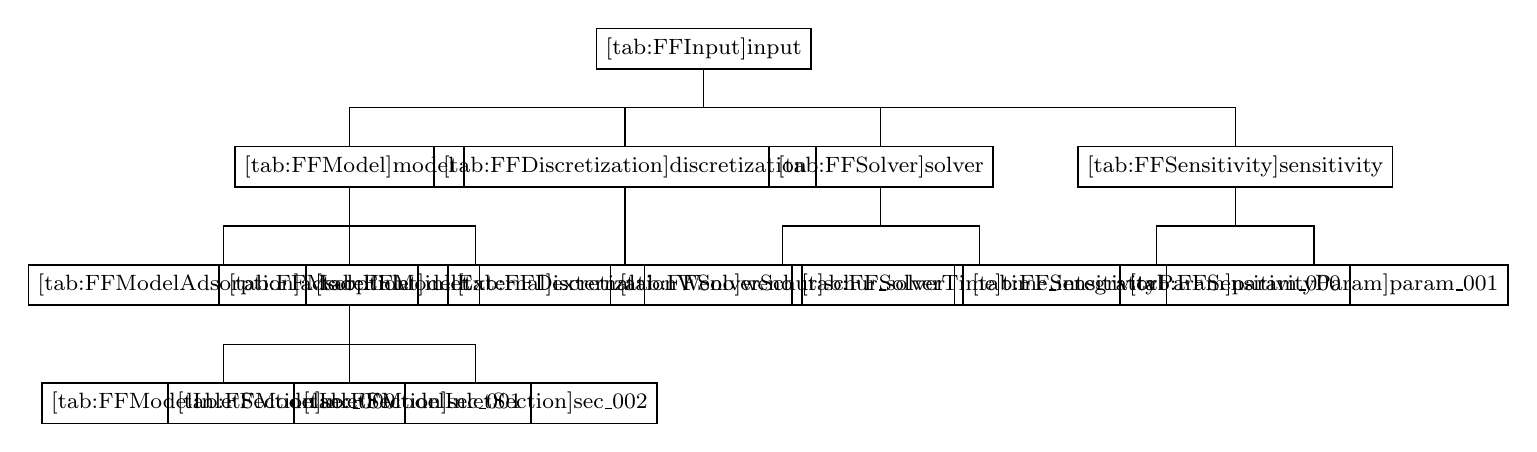
\begin{tikzpicture}[%
  every node/.style={draw=black,semithick,font=\footnotesize},
  level 2/.style={sibling distance=16mm},
  ]
  \node {\hyperref[tab:FFInput]{input}} [edge from parent fork down]
    child[sibling distance=30mm] { node {\hyperref[tab:FFModel]{model} } [edge from parent fork down]
              child { node { \hyperref[tab:FFModelAdsorption]{adsorption} } }
              child { node { \hyperref[tab:FFModelInlet]{inlet} } [edge from parent fork down]
                        child { node { \hyperref[tab:FFModelInletSection]{sec\_000} } }
                        child { node { \hyperref[tab:FFModelInletSection]{sec\_001} } }
                        child { node { \hyperref[tab:FFModelInletSection]{sec\_002} } }
                    }
              child { node { \hyperref[tab:FFModelExternal]{external} } }
          }   
    child[sibling distance=20mm] { node { \hyperref[tab:FFDiscretization]{discretization} } [edge from parent fork down]
              child { node { \hyperref[tab:FFDiscretizationWeno]{weno} } }
          }
    child[sibling distance=45mm] { node { \hyperref[tab:FFSolver]{solver} } [edge from parent fork down]
              child[sibling distance=25mm] { node { \hyperref[tab:FFSolverSchur]{schur\_solver} } }
              child[sibling distance=25mm] { node { \hyperref[tab:FFSolverTime]{time\_integrator} } }
          }
    child[sibling distance=45mm] { node { \hyperref[tab:FFSensitivity]{sensitivity} } [edge from parent fork down]
              child[sibling distance=20mm] { node { \hyperref[tab:FFSensitivityParam]{param\_000} } }
              child[sibling distance=20mm] { node { \hyperref[tab:FFSensitivityParam]{param\_001} } }
          };
\end{tikzpicture}
\caption{\label{fig:FFInput}Structure of the groups in the input part of the file format}
\end{figure}

\begin{figure}[!ht]
\centering
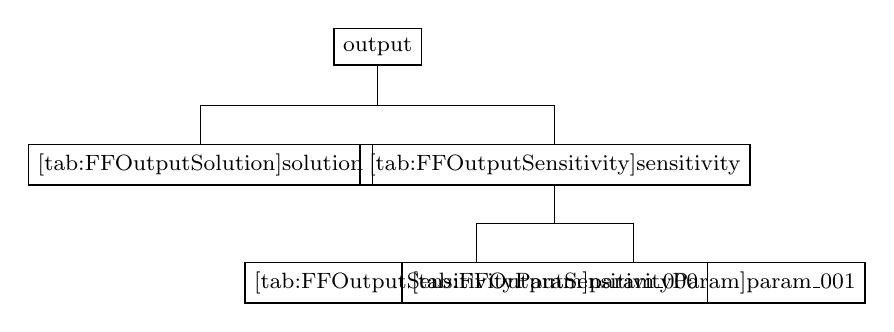
\begin{tikzpicture}[%
  every node/.style={draw=black,semithick,font=\footnotesize},
  ]
  \node {output} [edge from parent fork down]
    child[sibling distance=45mm] { node { \hyperref[tab:FFOutputSolution]{solution} } }   
    child[sibling distance=45mm] { node { \hyperref[tab:FFOutputSensitivity]{sensitivity} } [edge from parent fork down]
              child[sibling distance=20mm] { node { \hyperref[tab:FFOutputSensitivityParam]{param\_000} } }
              child[sibling distance=20mm] { node { \hyperref[tab:FFOutputSensitivityParam]{param\_001} } }
          };
\end{tikzpicture}
\caption{\label{fig:FFOutput}Structure of the groups in the output part of the file format}
\end{figure}

\subsection{Description of datasets}

Reference volumes are denoted by subscripts:
\begin{itemize}
  \item[\si{\cubic\metre\of{Int}}] Interstitial volume
  \item[\si{\cubic\metre\of{MP}}] Bead mobile phase volume
  \item[\si{\cubic\metre\of{SP}}] Bead solid phase volume
\end{itemize}

\newpage

\newcommand{\GroupHeadline}[1]{\small\textbf{Group} \texttt{#1}}

\begin{table}[!ht]
\footnotesize
\begin{tabu}to \linewidth[m]{lXcc} \toprule
\multicolumn{4}{c}{\GroupHeadline{/input}} \\
\rowfont[c]\normalfont Dataset & Description & Type & Range \everyrow{\midrule}\\
\texttt{CHROMATOGRAPHY\_TYPE} & Specifies the type of mass transport model & string &
      \texttt{GENERAL\_RATE\_MODEL} \everyrow{}\\
\bottomrule
\end{tabu}
\caption{\label{tab:FFInput}Datasets in the \texttt{/input} group}
\end{table}

\begin{table}[!ht]
\footnotesize
\begin{tabu}to \linewidth[m]{lX[m]cccc} \toprule
\multicolumn{6}{c}{\GroupHeadline{/input/model}} \\
\rowfont[c]\normalfont Dataset & Description & Unit & Type & Range & Length \everyrow{\midrule}\\
\texttt{NCOMP}& Number of chemical components in the chromatographic media & -- & int  & $\geq 1$ & 1 \\
\texttt{ADSORPTION\_TYPE} & Specifies the type of adsorption model & -- & string & See Table~\ref{tab:FFModelAdsorption} & 1 \\
\texttt{INIT\_C} & A vector with initial concentrations for each comp.\ in the mobile phase & \si{\mol\per\cubic\metre\of{Int \& MP}} & double & $\geq 0.0$ & \texttt{NCOMP}\\
\texttt{INIT\_Q} & Same as \texttt{INIT\_C} but for the bound phase & \si{\mol\per\cubic\metre\of{SP}} & double & $\geq 0.0$ & \texttt{NCOMP}\\
\texttt{COL\_DISPERSION} & Axial dispersion coefficient & \si{\square\metre\of{Int}\per\second} & double & $\geq 0.0$ & 1 / \texttt{NSEC}\\
\texttt{COL\_LENGTH} & Column length & \si{\metre} & double & $> 0.0$ & 1\\
\texttt{COL\_POROSITY} & Column porosity & -- & double & $\geq 0.0$ & 1\\
\texttt{FILM\_DIFFUSION} & A vector with film diffusion coefficients & \si{\metre\per\second} & double & $\geq 0.0$ & \texttt{NCOMP} / {$\texttt{NCOMP} \times \texttt{NSEC}$}\\
\texttt{PAR\_DIFFUSION} & A vector with particle diffusion coefficients & \si{\square\metre\of{MP}\per\second} & double & $\geq 0.0$ & \texttt{NCOMP} / {$\texttt{NCOMP} \times \texttt{NSEC}$}\\
\texttt{PAR\_POROSITY} & Particle porosity & -- & double & $> 0.0$ & 1\\
\texttt{PAR\_RADIUS} & Particle radius & \si{\metre} & double & $> 0.0$ & 1\\
\texttt{PAR\_SURFDIFFUSION} & A vector with particle surface diffusion coefficients & \si{\square\metre\of{SP}\per\second} & double & $\geq 0.0$ & \texttt{NCOMP} / {$\texttt{NCOMP} \times \texttt{NSEC}$}\\
\texttt{VELOCITY} & Interstitial velocity of the mobile phase & \si{\metre\per\second} & double & $> 0.0$ & 1 / \texttt{NSEC}\everyrow{}\\
\bottomrule
\end{tabu}
\caption{\label{tab:FFModel}Datasets in the \texttt{/input/model} group}
\end{table}

\begin{footnotesize}
\tabulinesep=3pt
\begin{longtabu}to \linewidth[m]{l>{\scriptsize}X[m]cccc} \toprule
\multicolumn{6}{c}{\GroupHeadline{/input/model/adsorption}} \\
\rowfont[c]\normalfont Dataset & \normalsize Description & Unit & Type & Range & Length\\
\endfirsthead
%
\toprule
\multicolumn{6}{c}{\GroupHeadline{/input/model/adsorption} Continued} \\
\rowfont[c]\normalfont Dataset & \normalsize Description & Unit & Type & Range & Length\\
\midrule
\endhead
%
\bottomrule
\endfoot
%
\bottomrule
\caption{\label{tab:FFModelAdsorption}Datasets in the \texttt{/input/model/adsorption} group}\\
\endlastfoot
%\multicolumn{5}{c}{\texttt{/input/model/adsorption}} \\
%\rowfont[c]\normalfont Dataset & Description & Unit & Type & Range\\
\midrule
\texttt{IS\_KINETIC} & Selects kinetic or stationary adsorbance mode: 1 = kinetic, 0 = stationary & -- & int & 0/1 & 1\\
\midrule
\multicolumn{6}{l}{If \texttt{ADSORPTION\_MODEL} = \texttt{LINEAR}:} \\ % Top level heading
\midrule
\texttt{LIN\_KA} & A vector with adsorption rate constants in the linear binding model & \si{\cubic\metre\of{MP}\per\cubic\metre\of{SP}\per\second} & double & $\geq 0.0$ & \texttt{NCOMP}\\
\midrule
\texttt{LIN\_KD} & A vector with desorption rate constants in the linear binding model & \si{\per\second} & double & $\geq 0.0$ & \texttt{NCOMP}\\
\midrule
\multicolumn{6}{l}{If \texttt{ADSORPTION\_MODEL} = \texttt{MULTI\_COMPONENT\_LANGMUIR}:} \\ % Top level heading
\midrule
\texttt{MCL\_KA} & A vector with adsorption rate constants in the multi component langmuir model & \si{\cubic\metre\of{MP}\per\mol\per\second} & double & $\geq 0.0$ & \texttt{NCOMP}\\
\midrule
\texttt{MCL\_KD} & A vector with desorption rate constants in the multi component langmuir model & \si{\per\second} & double & $\geq 0.0$ & \texttt{NCOMP}\\
\midrule
\texttt{MCL\_QMAX} & A vector with maximum adsorption capacities in the multi component langmuir model & \si{\mol\per\cubic\metre\of{SP}} & double & $> 0.0$ & \texttt{NCOMP}\\
\midrule
\multicolumn{6}{l}{If \texttt{ADSORPTION\_MODEL} = \texttt{MOBILE\_PHASE\_MODULATORS}:} \\ % Top level heading
\midrule
\texttt{MPM\_KA} & A vector with adsorption rate constants in the mobile phase modulator model & \si{\cubic\metre\of{MP}\per\mol\per\second} & double & $\geq 0.0$ & \texttt{NCOMP}\\
\midrule
\texttt{MPM\_KD} & A vector with desorption rate constants in the mobile phase modulator model & \si{\raiseto{3\beta}\metre\of{MP}\per\raiseto{\beta}\mol\per\second} & double & $\geq 0.0$ & \texttt{NCOMP}\\
\midrule
\texttt{MPM\_QMAX} & A vector with maximum adsorption capacities in the mobile phase modulator model & \si{\mol\per\cubic\metre\of{SP}} & double & $\geq 0.0$ & \texttt{NCOMP}\\
\midrule
\texttt{MPM\_BETA} & A vector with parameters describing the ion-exchange characteristics (IEX) & -- & double & $\geq 0.0$ & \texttt{NCOMP}\\
\midrule
\texttt{MPM\_GAMMA} & A vector with parameters describing the hydrophobicity (HIC) & \si{\cubic\metre\of{MP}\per\mol} & double & $\geq 0.0$ & \texttt{NCOMP}\\
\midrule
\multicolumn{6}{l}{If \texttt{ADSORPTION\_MODEL} = \texttt{EXTERNAL\_LANGMUIR}:} \\ % Top level heading
\midrule
\begin{tabular}{c}
  \texttt{EXTL\_KA} \\
  \texttt{EXTL\_KA\_T} \\
  \texttt{EXTL\_KA\_TT} \\
  \texttt{EXTL\_KA\_TTT} \\
\end{tabular} & All vectors with adsorption rate constant coefficients in the External Function Langmuir model & \begin{tabular}{c}
  \si{\cubic\metre\of{MP}\per\mol\per\second} \\
  \si{\cubic\metre\of{MP}\per\mol\per\second\per\ExternalUnit} \\
  \si{\cubic\metre\of{MP}\per\mol\per\second\per\raiseto{2}\ExternalUnit} \\
  \si{\cubic\metre\of{MP}\per\mol\per\second\per\raiseto{3}\ExternalUnit} \\
\end{tabular} & double & $-\infty - \infty$ & \texttt{NCOMP}\\
\midrule
\begin{tabular}{c}
  \texttt{EXTL\_KD} \\
  \texttt{EXTL\_KD\_T} \\
  \texttt{EXTL\_KD\_TT} \\
  \texttt{EXTL\_KD\_TTT} \\
\end{tabular} & All vectors with desorption rate constant coefficients in the External Function Langmuir model & \begin{tabular}{c}
  \si{\per\second} \\
  \si{\per\second\per\ExternalUnit} \\
  \si{\per\second\per\raiseto{2}\ExternalUnit} \\
  \si{\per\second\per\raiseto{3}\ExternalUnit} \\
\end{tabular} & double & $-\infty - \infty$ & \texttt{NCOMP}\\
\midrule
\begin{tabular}{c}
  \texttt{EXTL\_QMAX} \\
  \texttt{EXTL\_QMAX\_T} \\
  \texttt{EXTL\_QMAX\_TT} \\
  \texttt{EXTL\_QMAX\_TTT} \\
\end{tabular} & All vectors with maximum adsorption capacity coefficients in the External Function Langmuir model & \begin{tabular}{c}
  \si{\mol\per\cubic\metre\of{SP}} \\
  \si{\mol\per\cubic\metre\of{SP}\per\ExternalUnit} \\
  \si{\mol\per\cubic\metre\of{SP}\per\raiseto{2}\ExternalUnit} \\
  \si{\mol\per\cubic\metre\of{SP}\per\raiseto{3}\ExternalUnit} \\
\end{tabular} & double & $-\infty - \infty$ & \texttt{NCOMP}\\
\midrule
\multicolumn{6}{l}{If \texttt{ADSORPTION\_MODEL} = \texttt{STERIC\_MASS\_ACTION}:} \\ % Top level heading
\midrule
\texttt{SMA\_LAMBDA} & Stationary phase capacity (monovalent salt counterions); The total number of binding sites available on the resin surface & \si{\mol\per\cubic\metre\of{SP}} & double & $\geq 0.0$ & 1\\
\midrule
\texttt{SMA\_KA} & A vector with adsorption rate constants in the steric mass action model & \si{\raiseto{3(\nu_i-1)}\metre\of{SP}\raiseto{3}\metre\of{MP}\per\raiseto{\nu_i}\mol\per\second} & double & $\geq 0.0$ & \texttt{NCOMP}\\
\midrule
\texttt{SMA\_KD} & A vector with desorption rate constants in the steric mass action model & \si{\raiseto{3\nu_i}\metre\of{MP}\per\raiseto{\nu_i}\mol\per\second} & double & $\geq 0.0$ & \texttt{NCOMP}\\
\midrule
\texttt{SMA\_NU} & A vector with characteristic charges of the protein; The number of sites $\nu$ that the protein interacts with on the resin surface & -- & double & $\geq 0.0$ & \texttt{NCOMP}\\
\midrule
\texttt{SMA\_SIGMA} & A vector with steric factors of the protein; The number of sites $\sigma$ on the surface that are shielded by the protein and prevented from exchange with the salt counterions in solution & -- & double & $\geq 0.0$ & \texttt{NCOMP}\\
\midrule
\multicolumn{6}{l}{If \texttt{ADSORPTION\_MODEL} = \texttt{SELF\_ASSOCIATION}:} \\ % Top level heading
\midrule
\texttt{SAI\_LAMBDA} & Stationary phase capacity (monovalent salt counterions); The total number of binding sites available on the resin surface & \si{\mol\per\cubic\metre\of{SP}} & double & $\geq 0.0$ & 1\\
\midrule
\texttt{SAI\_KA1} & A vector with adsorption rate constants in the self association model & \si{\raiseto{3(\nu_i-1)}\metre\of{SP}\raiseto{3}\metre\of{MP}\per\raiseto{\nu_i}\mol\per\second} & double & $\geq 0.0$ & \texttt{NCOMP}\\
\midrule
\texttt{SAI\_KA2} & A vector with adsorption rate constants of dimerization in the self association model & \si{\raiseto{3(\nu_i-1)}\metre\of{SP}\raiseto{6}\metre\of{MP}\per\raiseto{(\nu_i+1)}\mol\per\second}  & double & $\geq 0.0$ & \texttt{NCOMP}\\
\midrule
\texttt{SAI\_KD} & A vector with desorption rate constants in the self association model & \si{\raiseto{3\nu_i}\metre\of{MP}\per\raiseto{\nu_i}\mol\per\second} & double & $\geq 0.0$ & \texttt{NCOMP}\\
\midrule
\texttt{SAI\_NU} & A vector with characteristic charges $\nu$ of the protein & -- & double & $\geq 0.0$ & \texttt{NCOMP}\\
\midrule
\texttt{SAI\_SIGMA} & A vector with steric factors $\sigma$ of the protein & -- & double & $\geq 0.0$ & \texttt{NCOMP}\\
\midrule
\multicolumn{6}{l}{If \texttt{ADSORPTION\_MODEL} = \texttt{EXTERNAL\_STERIC\_MASS\_ACTION}:} \\ % Top level heading
\midrule
\begin{tabular}{@{}l@{}}
  \texttt{EXTSMA\_KA} \\
  \texttt{EXTSMA\_KA\_T} \\
  \texttt{EXTSMA\_KA\_TT} \\
  \texttt{EXTSMA\_KA\_TTT} \\
\end{tabular} & All vectors with adsorption rate constants in the thermal steric mass action model & \begin{tabular}{@{}l@{}}
  \si{\raiseto{3(\nu_i-1)}\metre\of{SP}\raiseto{3}\metre\of{MP}\per\raiseto{\nu_i}\mol\per\second} \\
  \si{\raiseto{3(\nu_i-1)}\metre\of{SP}\raiseto{3}\metre\of{MP}\per\raiseto{\nu_i}\mol\per\second\per\ExternalUnit} \\
  \si{\raiseto{3(\nu_i-1)}\metre\of{SP}\raiseto{3}\metre\of{MP}\per\raiseto{\nu_i}\mol\per\second\per\raiseto{2}\ExternalUnit} \\
  \si{\raiseto{3(\nu_i-1)}\metre\of{SP}\raiseto{3}\metre\of{MP}\per\raiseto{\nu_i}\mol\per\second\per\raiseto{3}\ExternalUnit} \\
\end{tabular} & double & $-\infty - \infty$ & \texttt{NCOMP}\\
\midrule 
\begin{tabular}{@{}l@{}}
  \texttt{EXTSMA\_KD} \\
  \texttt{EXTSMA\_KD\_T} \\
  \texttt{EXTSMA\_KD\_TT} \\
  \texttt{EXTSMA\_KD\_TTT} \\
\end{tabular} & All vectors with desorption rate constant coefficients in the thermal steric mass action model & \begin{tabular}{@{}l@{}}
  \si{\raiseto{3\nu_i}\metre\of{MP}\per\raiseto{\nu_i}\mol\per\second} \\
  \si{\raiseto{3\nu_i}\metre\of{MP}\per\raiseto{\nu_i}\mol\per\second\per\ExternalUnit} \\
  \si{\raiseto{3\nu_i}\metre\of{MP}\per\raiseto{\nu_i}\mol\per\second\per\raiseto{2}\ExternalUnit} \\
  \si{\raiseto{3\nu_i}\metre\of{MP}\per\raiseto{\nu_i}\mol\per\second\per\raiseto{3}\ExternalUnit} \\
\end{tabular} & double & $-\infty - \infty$ & \texttt{NCOMP}\\
\midrule
\begin{tabular}{@{}l@{}}
  \texttt{EXTSMA\_NU} \\
  \texttt{EXTSMA\_NU\_T} \\
  \texttt{EXTSMA\_NU\_TT} \\
  \texttt{EXTSMA\_NU\_TTT} \\
\end{tabular} & All vectors with characteristic charges of the protein in the thermal steric mass action model & \begin{tabular}{@{}l@{}}
  --\\
  \si{\per\ExternalUnit} \\
  \si{\per\raiseto{2}\ExternalUnit} \\
  \si{\per\raiseto{3}\ExternalUnit} \\
\end{tabular} & double & $-\infty - \infty$ & \texttt{NCOMP}\\
\midrule
\begin{tabular}{@{}l@{}}
  \texttt{EXTSMA\_SIGMA} \\
  \texttt{EXTSMA\_SIGMA\_T} \\
  \texttt{EXTSMA\_SIGMA\_TT} \\
  \texttt{EXTSMA\_SIGMA\_TTT} \\
\end{tabular} & All vectors with steric factors of the protein in the thermal steric mass action model & \begin{tabular}{@{}l@{}}
  --\\
  \si{\per\ExternalUnit} \\
  \si{\per\raiseto{2}\ExternalUnit} \\
  \si{\per\raiseto{3}\ExternalUnit} \\
\end{tabular} & double & $-\infty - \infty$ & \texttt{NCOMP}\\
\midrule
\begin{tabular}{@{}l@{}}
  \texttt{EXTSMA\_LAMBDA} \\
  \texttt{EXTSMA\_LAMBDA\_T} \\
  \texttt{EXTSMA\_LAMBDA\_TT} \\
  \texttt{EXTSMA\_LAMBDA\_TTT} \\
\end{tabular} & Stationary phase capacity (monovalent salt counterions) in the thermal steric mass action model & \begin{tabular}{@{}l@{}}
  \si{\mol\per\cubic\metre\of{SP}}\\
  \si{\mol\per\cubic\metre\of{SP}\per\ExternalUnit} \\
  \si{\mol\per\cubic\metre\of{SP}\per\raiseto{2}\ExternalUnit} \\
  \si{\mol\per\cubic\metre\of{SP}\per\raiseto{3}\ExternalUnit} \\
\end{tabular} & double & $-\infty - \infty$ & 1\\
\midrule
\multicolumn{6}{l}{If \texttt{ADSORPTION\_MODEL} = \texttt{MULTI\_COMPONENT\_BILANGMUIR}:} \\ % Top level heading
\midrule
\texttt{MCBL\_KA1} & A vector with adsorption rate constants of the first binding site type in the multi component Bi-Langmuir model & \si{\cubic\metre\of{MP}\per\mol\per\second} & double & $\geq 0.0$ & \texttt{NCOMP} / 2 \\
\midrule
\texttt{MCBL\_KA2} & A vector with adsorption rate constants of the second binding site type in the multi component Bi-Langmuir model & \si{\cubic\metre\of{MP}\per\mol\per\second} & double & $\geq 0.0$ & \texttt{NCOMP} / 2 \\
\midrule
\texttt{MCBL\_KD1} & A vector with desorption rate constants of the first binding site type in the multi component Bi-Langmuir model & \si{\per\second} & double & $\geq 0.0$ & \texttt{NCOMP} / 2\\
\midrule
\texttt{MCBL\_KD2} & A vector with desorption rate constants of the second binding site type in the multi component Bi-Langmuir model & \si{\per\second} & double & $\geq 0.0$ & \texttt{NCOMP} / 2\\
\midrule
\texttt{MCBL\_QMAX1} & A vector with with maximum adsorption capacities of the first binding site type & \si{\mol\per\cubic\metre\of{SP}} & double & $> 0.0$ & \texttt{NCOMP} / 2\\
\midrule
\texttt{MCBL\_QMAX2} & A vector with with maximum adsorption capacities of the second binding site type & \si{\mol\per\cubic\metre\of{SP}} & double & $> 0.0$ & \texttt{NCOMP} / 2 \everyrow{}\\
\end{longtabu}
\end{footnotesize}


\begin{table}[!ht]
\footnotesize
\begin{tabu}to \linewidth[m]{lX[m]cccc} \toprule
\multicolumn{6}{c}{\GroupHeadline{/input/model/inlet}} \\
\rowfont[c]\normalfont Dataset & Description & Unit & Type & Range & Length \everyrow{\midrule}\\
\texttt{NSEC} & Number of sections & -- & int & $\geq 1$ & 1\\
\texttt{SECTION\_TIMES} & A vector with simulation times at which inlet function is discontinous; including start and end times & \si{\second} & double & $\geq 0.0$ & \texttt{NSEC}+1\\
\texttt{SECTION\_CONTINUITY} & A vector indicating continuity of each section transition & -- & int &  
  \begin{tabular}{c}
    0 (discontinuous) \\
    1 (continuous)
  \end{tabular} & \texttt{NSEC}-1
\everyrow{}\\
\bottomrule
\end{tabu}
\caption{\label{tab:FFModelInlet}Datasets in the \texttt{/input/model/inlet} group}
\end{table}


\begin{table}[!ht]
\footnotesize
\begin{tabu}to \linewidth[m]{lX[m]cccc} \toprule
\multicolumn{6}{c}{\GroupHeadline{/input/model/inlet/sec\_XXX}} \\
\rowfont[c]\normalfont Dataset & Description & Unit & Type & Range & Length \everyrow{\midrule}\\
\texttt{CONST\_COEFF} & A vector with constant coefficients for inlet concentrations & \si{\mol\per\cubic\metre\of{Int}} & double & $-\infty - \infty$ & \texttt{NCOMP} \\
\texttt{LIN\_COEFF} & A vector with linear coefficients for inlet concentrations & \si{\mol\per\cubic\metre\of{Int}\per\second} & double & $-\infty - \infty$ & \texttt{NCOMP} \\
\texttt{QUAD\_COEFF} & A vector with quadratic coefficients for inlet concentrations & \si{\mol\per\cubic\metre\of{Int}\per\square\second} & double & $-\infty - \infty$ & \texttt{NCOMP} \\
\texttt{CUBE\_COEFF} & A vector with cubic coefficients for inlet concentrations & \si{\mol\per\cubic\metre\of{Int}\per\cubic\second} & double & $-\infty - \infty$ & \texttt{NCOMP} 
\everyrow{}\\
\bottomrule
\end{tabu}
\caption{\label{tab:FFModelInletSection}Datasets in the \texttt{/input/model/inlet/sec\_XXX} groups}
\end{table}


\begin{table}[!ht]
\footnotesize
\begin{tabu}to \linewidth[m]{lX[m]cccc} \toprule
\multicolumn{6}{c}{\GroupHeadline{/input/model/external}} \\
\rowfont[c]\normalfont Dataset & Description & Unit & Type & Range & Length \everyrow{\midrule}\\
\texttt{EXT\_VELOCITY} & Velocity of the external profile in positive column axial direction & \si{\metre\per\second} & double & $-\infty - \infty$ & 1\\
\texttt{EXT\_PROFILE} & A vector with external measurements $T$ & \si{\ExternalUnit} & double & $\geq 0$ & Arbitrary\\
\texttt{EXT\_PROF\_DELTA} & A vector with distances of the external measurements (first entry must be $0.0$) & \si{\metre} & double & $\geq 0.0$ & Same as \texttt{EXT\_PROFILE}
\everyrow{}\\
\bottomrule
\end{tabu}
\caption{\label{tab:FFModelExternal}Datasets in the \texttt{/input/model/external} group}
\end{table}


\begin{table}[!ht]
\footnotesize
\begin{tabu}to \linewidth[m]{lX[m]cccc} \toprule
\multicolumn{6}{c}{\GroupHeadline{/input/discretization}} \\
\rowfont[c]\normalfont Dataset & Description & Unit & Type & Range & Length \everyrow{\midrule}\\
\texttt{NCOL} & Number of column (axial) discretization cells & -- & int & $\geq 1$ & 1\\
\texttt{NPAR} & Number of particle (radial) discretization cells & -- & int & $\geq 1$ & 1\\
\texttt{PAR\_DISC\_TYPE} & Specifies the discretization scheme inside the particles & -- & string
& \begin{tabular}{c}
  \texttt{EQUIDISTANT\_PAR} \\
  \texttt{EQUIVOLUME\_PAR} \\
  \texttt{USER\_DEFINED\_PAR} \\
  \end{tabular} & 1\\
\texttt{PAR\_DISC\_VECTOR} & A vector with node coordinates for the cell boundaries & \si{\metre} & double
  & $0.0-1.0$ & \texttt{NPAR}+1 \\
\texttt{RECONSTRUCTION} & Type of reconstruction method for fluxes & -- & string
& \begin{tabular}{c}
  \texttt{WENO}
  \end{tabular} & 1\everyrow{}\\
\bottomrule
\end{tabu}
\caption{\label{tab:FFDiscretization}Datasets in the \texttt{/input/discretization} group}
\end{table}


\begin{table}[!ht]
\footnotesize
\begin{tabu}to \linewidth[m]{lX[m]cc} \toprule
\multicolumn{4}{c}{\GroupHeadline{/input/discretization/weno}} \\
\rowfont[c]\normalfont Dataset & Description & Type & Range \everyrow{\midrule}\\
\texttt{BOUNDARY\_MODEL} & Boundary model type: 0 = Lower WENO order (stable), 1 = Zero weights (unstable for small $D_{ax}$), 2 = Zero weights for p $\neq$ 0 (stable?), 3 = Large ghost points & int & $0-3$\\
\texttt{WENO\_EPS} & WENO $\varepsilon$ & double & $\geq 0.0$\\
\texttt{WENO\_ORDER} & WENO Order: 1 = standard upwind scheme, 2, 3; also called WENO K & int & $1-3$ \everyrow{}\\
\bottomrule
\end{tabu}
\caption{\label{tab:FFDiscretizationWeno}Datasets in the \texttt{/input/discretization/weno} group}
\end{table}


\begin{table}[!ht]
\footnotesize
\begin{tabu}to \linewidth[m]{lX[m]ccc} \toprule
\multicolumn{5}{c}{\GroupHeadline{/input/solver}} \\
\rowfont[c]\normalfont Dataset & Description & Unit & Type & Range \everyrow{\midrule}\\      
\texttt{NTHREADS} & Number of used OpenMP threads & -- & int & $\geq 1$ \\
\texttt{LOG\_LEVEL} & Specifies the verbosity of the logging output (Only errors;
warning and errors; info and warnings and errors, etc.) & -- & string &
\begin{tabular}{@{}c@{}} \texttt{ERROR} \\
  \texttt{WARNING} \\
  \texttt{INFO} \\
  \texttt{DEBUG1} \\
  \texttt{DEBUG2} \\
  \texttt{TRACE1} \\
  \texttt{TRACE2} \\
\end{tabular} \\
\texttt{PRINT\_CONFIG} & Print configuration message before simulation & -- & int & 0/1 \\
\texttt{PRINT\_PARAMLIST} & Print list of parameters before simulation & -- & int & 0/1 \\
\texttt{PRINT\_PROGRESS} & Print current state of simulation & -- & int & 0/1 \\
\texttt{PRINT\_STATISTICS} & Print integrator statistics after each section & -- & int & 0/1 \\
\texttt{PRINT\_TIMING} & Print timing information after simulation & -- & int & 0/1 \\
\texttt{USE\_ANALYTIC\_JACOBIAN} & Use analytically computed jacobian matrix (faster) instead of jacobian generated by algorithmic differentiation (slower) & -- & int & 0/1 \\
\texttt{USER\_SOLUTION\_TIMES} & A \emph{vector} with timepoints at which a solution is desired & \si{\second} & double & $\geq 0.0$ \\
\texttt{WRITE\_AT\_USER\_TIMES} & Write solutions at times specified by \texttt{USER\_SOLUTION\_TIMES} (write integration timepoints otherwise) & -- & int & 0/1 \\
\texttt{WRITE\_SOLUTION\_TIMES} & Write times at which a solution was produced & -- & int & 0/1 \\
\texttt{WRITE\_SOLUTION\_COLUMN\_INLET} & Write solutions at column inlet (boundary condition) & -- & int & 0/1 \\
\texttt{WRITE\_SOLUTION\_COLUMN\_OUTLET} & Write solutions at column outlet (chromatograms) & -- & int & 0/1 \\
\texttt{WRITE\_SOLUTION\_ALL} & Write all (intermediate) solutions & -- & int & 0/1 \\
\texttt{WRITE\_SENS\_COLUMN\_OUTLET} & Write sensitivity data at column outlet & -- & int & 0/1 \\
\texttt{WRITE\_SENS\_ALL} & Write all (intermediate) sensitivity data & -- & int & 0/1 \everyrow{}\\
\bottomrule
\end{tabu}
\caption{\label{tab:FFSolver}Datasets in the \texttt{/input/solver} group}
\end{table}


\begin{table}[!ht]
\footnotesize
\begin{tabu}to \linewidth[m]{lX[m]cc} \toprule
\multicolumn{4}{c}{\GroupHeadline{/input/solver/schur\_solver}} \\
\rowfont[c]\normalfont Dataset & Description & Type & Range \everyrow{\midrule}\\      
\texttt{GS\_TYPE} & Type of Gram-Schmidt orthogonalization, see IDAS guide
4.5.7.3, 41f. & int &
\begin{tabular}{c}
  0 (\texttt{CLASSICAL\_GS}) \\
  1 (\texttt{MODIFIED\_GS})
\end{tabular} \\
\texttt{MAX\_KRYLOV} & Defines the size of the iterative linear SPGMR solver (0: \texttt{MAX\_KRYLOV} = \texttt{NCOL}) & int & $0-\texttt{NCOL}$\\
\texttt{MAX\_RESTARTS} & Maximum number of restarts in the GMRES algorithm. If lack of memory isn't an issue, better use a larger Krylov space than restarts & int & $\geq 0$ \\
\texttt{SCHUR\_SAFETY} & Schur safety factor; Influences the tradeof between linear iterations and nonlinear error control; see IDAS guide 2.1, 5 & double & $\geq 0.0$ \everyrow{}\\
\bottomrule
\end{tabu}
\caption{\label{tab:FFSolverSchur}Datasets in the \texttt{/input/solver/schur\_solver} group}
\end{table}


\begin{table}[!ht]
\footnotesize
\begin{tabu}to \linewidth[m]{lX[m]cc} \toprule
\multicolumn{4}{c}{\GroupHeadline{/input/solver/time\_integrator}} \\
\rowfont[c]\normalfont Dataset & Description & Type & Range \everyrow{\midrule}\\      
\texttt{ABSTOL} & Absolute tolerance in the solution of the original system & double & $>0.0$\\
\texttt{RELTOL} & Relative tolerance in the solution of the original system & double & $\geq 0.0$\\
\texttt{INIT\_STEP\_SIZE} & Factor which is multiplied by the section length to get initial integrator stepsize (0.0: IDAS default value), see IDAS guide 4.5, 36f. & double & $0.0-1.0$\\
\texttt{MAX\_STEPS} & Maximum number of timesteps taken by IDAS (0: IDAS default = 500), see IDAS guide 4.5, 36 & int & $\geq 0$ \everyrow{}\\
\bottomrule
\end{tabu}
\caption{\label{tab:FFSolverTime}Datasets in the \texttt{/input/solver/time\_integrator} group}
\end{table}


\begin{table}[!ht]
\footnotesize
\begin{tabu}to \linewidth[m]{lX[m]cc} \toprule
\multicolumn{4}{c}{\GroupHeadline{/input/sensitivity}} \\
\rowfont[c]\normalfont Dataset & Description & Type & Range \everyrow{\midrule}\\      
\texttt{NSENS} & Number of sensitivities to be computed & int & $\geq 0$\\
\texttt{SENS\_METHOD} & Method used for computation of sensitivities; algorithmic differentiation or finite differences of order $1-4$ & string
& \begin{tabular}{@{}c@{}}
  \texttt{ad1} \\
  \texttt{fd1} \\
  \texttt{fd2} \\
  \texttt{fd4} \\
  \end{tabular} \everyrow{}\\
\bottomrule
\end{tabu}
\caption{\label{tab:FFSensitivity}Datasets in the \texttt{/input/sensitivity} group}
\end{table}


\begin{table}[!ht]
\footnotesize
\begin{tabu}to \linewidth[m]{lX[m]cc} \toprule
\multicolumn{4}{c}{\GroupHeadline{/input/sensitivity/param\_XXX}} \\
\rowfont[c]\normalfont Dataset & Description & Type & Range \everyrow{\midrule}\\      
\texttt{SENS\_NAME} & Name of the parameter & string & *\footnote{All parameter names allowed that occur in group \texttt{input\_model} except \texttt{NCOMP}, \texttt{INIT\_C}, \texttt{INIT\_Q}, \texttt{ADSORPTION\_TYPE}, \texttt{adsorption/IS\_KINETIC}, \texttt{inlet/NSEC}, \texttt{inlet/SECTION\_TIMES}, \texttt{inlet/SECTION\_CONTINUITY}, and everything in \texttt{external/}} \\
\texttt{SENS\_COMP} & Component index; only for parameters defined for each component (-1 otherwise) & int & $\geq -1$\\
\texttt{SENS\_SECTION} & Section index; only for inlet parameters (-1 otherwise) & int & $\geq -1$\\
\texttt{SENS\_ABSTOL} & Absolute tolerance used in the computation of the sensitivities. Rule of thumb: \texttt{ABSTOL} / \texttt{PARAM\_VALUE} & double & $\geq 0.0$\\
\texttt{SENS\_FD\_DELTA} & Relative disturbance $\Delta p$ in finite difference sensitivity computations & double & $\geq 0.0$\everyrow{}\\
\bottomrule
\end{tabu}
\caption{\label{tab:FFSensitivityParam}Datasets in the \texttt{/input/sensitivity/param\_XXX} groups}
\end{table}


\begin{table}[!ht]
\footnotesize
\begin{tabu}to \linewidth[m]{lX[m]cc} \toprule
\multicolumn{4}{c}{\GroupHeadline{/output/solution}} \\
\rowfont[c]\normalfont Dataset & Description & Unit & Type \everyrow{\midrule}\\      
\texttt{SOLUTION\_TIMES} & Time points at which the solution is written & \si{\second} & double \\
\texttt{SOLUTION\_COLUMN} & Interstitial solution as $n_{\text{Time}} \times n_{\text{Comp}} \times n_{\text{ColCells}}$ tensor in row-major storage & \si{\mol\per\cubic\metre\of{Int}} & double \\
\texttt{SOLUTION\_PARTICLE} & Solution inside the beads as $n_{\text{Time}} \times n_{\text{ColCells}} \times n_{\text{ParCells}} \times 2 \times n_{\text{Comp}}$ tensor in row-major storage & \si{\mol\per\cubic\metre\of{MP \& SP}} & double \\
\texttt{SOLUTION\_BOUNDARY} & Flux solution as $n_{\text{Time}} \times n_{\text{Comp}} \times n_{\text{ColCells}}$ tensor in row-major storage & \si{\mol\per\square\metre\per\second} & double \\
\texttt{SOLUTION\_COLUMN\_OUTLET\_COMP\_XXX} & Component \texttt{XXX} of the solution at the column outlet & \si{\mol\per\cubic\metre\of{Int}} & double \\
\texttt{SOLUTION\_COLUMN\_INLET\_COMP\_XXX} & Component \texttt{XXX} of the solution at the column inlet & \si{\mol\per\cubic\metre\of{Int}} & double 
\everyrow{}\\
\bottomrule
\end{tabu}
\caption{\label{tab:FFOutputSolution}Datasets in the \texttt{/output/solution} group}
\end{table}


\begin{table}[!ht]
\footnotesize
\begin{tabu}to \linewidth[m]{lX[m]cc} \toprule
\multicolumn{3}{c}{\GroupHeadline{/output/sensitivity}} \\
\rowfont[c]\normalfont Dataset & Description & Type \everyrow{\midrule}\\      
\texttt{SENS\_COLUMN} & Interstitial solution as $n_{\text{Time}} \times n_{\text{Comp}} \times n_{\text{ColCells}} \times n_{\text{Params}}$ tensor in row-major storage & double \\
\texttt{SENS\_PARTICLE} & Solution inside the beads as $n_{\text{Time}} \times n_{\text{ColCells}} \times n_{\text{ParCells}} \times 2 \times n_{\text{Comp}} \times n_{\text{Params}}$ tensor in row-major storage & double \\
\texttt{SENS\_BOUNDARY} & Flux solution as $n_{\text{Time}} \times n_{\text{Comp}} \times n_{\text{ColCells}} \times n_{\text{Params}}$ tensor in row-major storage & double
\everyrow{}\\
\bottomrule
\end{tabu}
\caption{\label{tab:FFOutputSensitivity}Datasets in the \texttt{/output/sensitivity} group}
\end{table}


\begin{table}[!ht]
\footnotesize
\begin{tabu}to \linewidth[m]{lX[m]cc} \toprule
\multicolumn{4}{c}{\GroupHeadline{/output/sensitivity/param\_XXX}} \\
\rowfont[c]\normalfont Dataset & Description & Unit & Type \everyrow{\midrule}\\      
\texttt{SENS\_COLUMN\_OUTLET\_COMP\_YYY} & Sensitivity of component \texttt{YYY} at the column outlet with respect to parameter \texttt{XXX} & \si{\mol\per\cubic\metre\of{Int}\per\ParamUnit} & double
\everyrow{}\\
\bottomrule
\end{tabu}
\caption{\label{tab:FFOutputSensitivityParam}Datasets in the \texttt{/output/sensitivity/param\_XXX} groups}
\end{table}


\FloatBarrier
\subsection{Section dependent model parameters}

Some model parameters (see Table~\ref{tab:FFSectionDependentParams}) can be assigned different values for each section. For example, the velocity the column is operated with could differ in the load, wash, and elution phases.
Section dependency is recognized by specifying the appropriate number of values for the parameters (see Length in Table~\ref{tab:FFModel}). 
If a parameter depends on the component and the section, the ordering is such that the values for the components are listed within each section (i.e., ``component-major''):
For example, in a three component system the ordering is \texttt{comp0sec0}, \texttt{comp1sec0}, \texttt{comp2sec0}, \texttt{comp0sec1}, \texttt{comp1sec1}, \texttt{comp2sec1}, \ldots

Note that single components of component dependent datasets cannot be section dependent.

\begin{table}[!ht]
\centering
\footnotesize
\begin{tabu}to \linewidth[m]{lcc} \toprule
\rowfont[c]\normalfont Dataset & Component dependent & Section dependent \everyrow{\midrule}\\      
\texttt{COL\_DISPERSION} & & \checkmark \\
\texttt{FILM\_DIFFUSION} & \checkmark  & \checkmark \\
\texttt{PAR\_DIFFUSION} & \checkmark  & \checkmark \\
\texttt{PAR\_SURFDIFFUSION} & \checkmark  & \checkmark \\
\texttt{VELOCITY} & & \checkmark \everyrow{}\\
\bottomrule
\end{tabu}
\caption{\label{tab:FFSectionDependentParams}Section dependent datasets in the \texttt{/input/model} group}
\end{table}


% =============================================================================
%  CADET - The Chromatography Analysis and Design Toolkit
%  
%  Copyright © 2008-2015: Eric von Lieres¹, Joel Andersson,
%                         Andreas Puettmann¹, Sebastian Schnittert¹,
%                         Samuel Leweke¹
%                                      
%    ¹ Forschungszentrum Juelich GmbH, IBG-1, Juelich, Germany.
%  
%  All rights reserved. This program and the accompanying materials
%  are made available under the terms of the GNU Public License v3.0 (or, at
%  your option, any later version) which accompanies this distribution, and
%  is available at http://www.gnu.org/licenses/gpl.html
% =============================================================================

\section{Isotherms}

\subsection{Linear}

\begin{align*}
  \frac{\mathrm{d} q_i}{\mathrm{d} t} = k_a c_{p,i} - k_d q_i && \forall i = 1, \dots, N_{\text{comp}}
\end{align*}

\begin{table}[!ht]
  \footnotesize
  \begin{tabu}to \linewidth[m]{lX[m]c}
    \toprule
      \textbf{Constant} & \textbf{Description} & \textbf{Unit} \\
    \midrule
      $k_a$ & Adsorption rate & \si{\cubic\metre\of{MP}\per\cubic\metre\of{SP}\per\second} \\ \midrule
      $k_d$ & Desorption rate & \si{\per\second} \\
    \bottomrule
  \end{tabu}
  \caption{Parameters of the linear adsorption model}
\end{table}

\subsection{Multi Component Langmuir}

\begin{align*}
  \frac{\mathrm{d} q_i}{\mathrm{d} t} = k_a\: c_{p,i}\: q_{\text{max},i} \left( 1 - \sum_{j=1}^{N_{\text{comp}}} \frac{q_j}{q_{\text{max},j}} \right) - k_d q_i && \forall i = 1, \dots, N_{\text{comp}}
\end{align*}

\begin{table}[!ht]
  \footnotesize
  \begin{tabu}to \linewidth[m]{lX[m]c}
    \toprule
      \textbf{Constant} & \textbf{Description} & \textbf{Unit} \\
    \midrule
      $k_a$ & Adsorption rate & \si{\cubic\metre\of{MP}\per\mol\per\second} \\ \midrule
      $k_d$ & Desorption rate & \si{\per\second} \\ \midrule
      $q_{\text{max}}$ & Maximum adsorption capacity; Maximum concentration & \si{\mol\per\cubic\metre\of{SP}} \\
    \bottomrule
  \end{tabu}
  \caption{Parameters of the Multi Component Langmuir adsorption model}
\end{table}

\subsection{Steric Mass Action}

\begin{align*}
  \frac{\mathrm{d} q_i}{\mathrm{d} t} = k_a c_{p,i}\left( \Lambda - \sum_{j=1}^{N_{\text{comp}}} \left( \nu_j + \sigma_j \right) q_j \right)^{\nu_i} - k_d\: q_i\: c_{p,0}^{\nu_i} && \forall i = 1, \dots, N_{\text{comp}}
\end{align*}
where $c_{p,0}$ and $q_0$ denote the salt concentrations in the liquid and solid phase of the beads respectively. A neutrality condition compensating for the missing equation for $\frac{\mathrm{d} q_0}{\mathrm{d}t}$ is required:
\begin{align*}
  q_0 = \Lambda - \sum_{j=1}^{N_{\text{comp}}} \nu_j q_j
\end{align*}

\begin{table}[!ht]
  \footnotesize
  \begin{tabu}to \linewidth[m]{lX[m]c}
    \toprule
      \textbf{Constant} & \textbf{Description} & \textbf{Unit} \\
    \midrule
      $\Lambda$ & Stationary phase capacity (monovalent salt counterions); The total number of binding sites available on the resin surface & \si{\mol\per\cubic\metre\of{SP}} \\ \midrule
      $k_a$ & Adsorption rate & \si{\raiseto{3(\nu_i-1)}\metre\of{SP}\raiseto{3}\metre\of{MP}\per\raiseto{\nu_i}\mol\per\second} \\ \midrule
      $k_d$ & Desorption rate & \si{\raiseto{3\nu_i}\metre\of{MP}\per\raiseto{\nu_i}\mol\per\second} \\ \midrule
      $\nu$ & Characteristic charges of the protein; The number of sites $\nu$ that the protein interacts with on the resin surface & -- \\ \midrule
      $\sigma$ & Steric factors of the protein; The number of sites $\sigma$ on the surface that are shielded by the protein and prevented from exchange with the salt counterions in solution & -- \\
    \bottomrule
  \end{tabu}
  \caption{Parameters of the Steric Mass Action adsorption model}
\end{table}

\subsection{Self Association}

\begin{align*}
  \frac{\mathrm{d} q_i}{\mathrm{d} t} = c_{p,i}\left( \Lambda - \sum_{j=1}^{N_{\text{comp}}} \left( \nu_j + \sigma_j \right) q_j \right)^{\nu_i} \left[ k_{a,1} + k_{a,2} c_{p,i} \right] - k_d\: q_i\: c_{p,0}^{\nu_i} && \forall i = 1, \dots, N_{\text{comp}}
\end{align*}
where $c_{p,0}$ and $q_0$ denote the salt concentrations in the liquid and solid phase of the beads respectively. A neutrality condition compensating for the missing equation for $\frac{\mathrm{d} q_0}{\mathrm{d}t}$ is required:
\begin{align*}
  q_0 = \Lambda - \sum_{j=1}^{N_{\text{comp}}} \nu_j q_j
\end{align*}

\begin{table}[!ht]
  \footnotesize
  \begin{tabu}to \linewidth[m]{lX[m]c}
    \toprule
      \textbf{Constant} & \textbf{Description} & \textbf{Unit} \\
    \midrule
      $\Lambda$ & Stationary phase capacity (monovalent salt counterions); The total number of binding sites available on the resin surface & \si{\mol\per\cubic\metre\of{SP}} \\ \midrule
      $k_{a,1}$ & Adsorption rate & \si{\raiseto{3(\nu_i-1)}\metre\of{SP}\raiseto{3}\metre\of{MP}\per\raiseto{\nu_i}\mol\per\second} \\ \midrule
      $k_{a,2}$ & Adsorption rate of dimerization & \si{\raiseto{3(\nu_i-1)}\metre\of{SP}\raiseto{6}\metre\of{MP}\per\raiseto{(\nu_i+1)}\mol\per\second} \\ \midrule
      $k_d$ & Desorption rate & \si{\raiseto{3\nu_i}\metre\of{MP}\per\raiseto{\nu_i}\mol\per\second} \\ \midrule
      $\nu$ & Characteristic charges of the protein; The number of sites $\nu$ that the protein interacts with on the resin surface & -- \\ \midrule
      $\sigma$ & Steric factors of the protein; The number of sites $\sigma$ on the surface that are shielded by the protein and prevented from exchange with the salt counterions in solution & -- \\
    \bottomrule
  \end{tabu}
  \caption{Parameters of the Self Association adsorption model}
\end{table}

\subsection{Mobile Phase Modulators Langmuir}

\begin{align*}
  \frac{\mathrm{d} q_i}{\mathrm{d} t} = k_a e^{\gamma c_{p,0}} c_{p,i}\: q_{\text{max},i} \left( 1 - \sum_{j=1}^{N_{\text{comp}}} \frac{q_j}{q_{\text{max},j}} \right) - k_d \: c_{p,0}^\beta \: q_i && \forall i = 1, \dots, N_{\text{comp}}
\end{align*}
where $c_{p,0}$ and $q_0$ denote the salt concentrations in the liquid and solid phase of the beads respectively. Salt is considered to be inert, therefore
\begin{align*}
  \frac{\mathrm{d} q_0}{\mathrm{d} t} = 0.
\end{align*}

\begin{table}[!ht]
  \footnotesize
  \begin{tabu}to \linewidth[m]{lX[m]c}
    \toprule
      \textbf{Constant} & \textbf{Description} & \textbf{Unit} \\
    \midrule
      $k_a$ & Adsorption rate & \si{\cubic\metre\of{MP}\per\mol\per\second} \\ \midrule
      $k_d$ & Desorption rate & \si{\raiseto{3\beta}\metre\of{MP}\per\raiseto{\beta}\mol\per\second} \\ \midrule
      $q_{\text{max}}$ & Maximum adsorption capacity; Maximum concentration & \si{\mol\per\cubic\metre\of{SP}} \\ \midrule
      $\gamma$ & Hydrophobicity & \si{\cubic\metre\of{MP}\per\mol} \\ \midrule
      $\beta$ & Describes ion-exchange characteristics & -- \\
    \bottomrule
  \end{tabu}
  \caption{Parameters of the Mobile Phase Modulators Langmuir adsorption model}
\end{table}

\subsection{External Function Multi Component Langmuir}

The same as ordinary Multi Component Langmuir but with coefficients $k_a$, $k_d$, and $q_{\text{max}}$ depending on an external quantity denoted by $T$:
\begin{align*}
  \frac{\mathrm{d} q_i}{\mathrm{d} t} = k_a(T)\: c_{p,i}\: q_{\text{max},i}(T) \left( 1 - \sum_{j=1}^{N_{\text{comp}}} \frac{q_j}{q_{\text{max},j}(T)} \right) - k_d(T) q_i && \forall i = 1, \dots, N_{\text{comp}}
\end{align*}
where the dependence is modeled by a polynomial of third degree, i.e.
\begin{align*}
  k_a(T) &= k_{a,3} T^3 + k_{a,2} T^2 + k_{a,1} T + k_{a,0}, \\
  k_d(T) &= k_{d,3} T^3 + k_{d,2} T^2 + k_{d,1} T + k_{d,0}, \\
  q_{\text{max}}(T) &= q_{\text{max},3} T^3 + q_{\text{max},2} T^2 + q_{\text{max},1} T + q_{\text{max},0}.
\end{align*}
The quantity $T(t, z)$ is a function of time $t$ and space $z$, i.e.\ $T\colon [0, t_{\text{max}}] \times [0, L] \rightarrow \mathds{R}$, which is externally given to the simulator.

\begin{table}[!ht]
  \footnotesize
  \begin{tabu}to \linewidth[m]{lX[m]c}
    \toprule
      \textbf{Constant} & \textbf{Description} & \textbf{Unit} \\
    \midrule
      $k_{a,3}$ & \multirow{4}{*}{Adsorption rate} & \si{\cubic\metre\of{MP}\per\mol\per\second\per\raiseto{3}\ExternalUnit} \\
      $k_{a,2}$ & & \si{\cubic\metre\of{MP}\per\mol\per\second\per\raiseto{2}\ExternalUnit} \\
      $k_{a,1}$ & & \si{\cubic\metre\of{MP}\per\mol\per\second\per\ExternalUnit} \\
      $k_{a,0}$ & & \si{\cubic\metre\of{MP}\per\mol\per\second} \\ \midrule
      $k_{d,3}$ & \multirow{4}{*}{Desorption rate} & \si{\per\second\per\raiseto{3}\ExternalUnit} \\
      $k_{d,2}$ & & \si{\per\second\per\raiseto{2}\ExternalUnit} \\
      $k_{d,1}$ & & \si{\per\second\per\ExternalUnit} \\
      $k_{d,0}$ & & \si{\per\second} \\ \midrule
      $q_{\text{max},3}$ & \multirow{4}{*}{Maximum adsorption capacity; Maximum concentration} & \si{\mol\per\cubic\metre\of{SP}\per\raiseto{3}\ExternalUnit} \\
      $q_{\text{max},2}$ & & \si{\mol\per\cubic\metre\of{SP}\per\raiseto{2}\ExternalUnit} \\
      $q_{\text{max},1}$ & & \si{\mol\per\cubic\metre\of{SP}\per\ExternalUnit} \\
      $q_{\text{max},0}$ & & \si{\mol\per\cubic\metre\of{SP}} \\ \midrule
      $T$ & External quantity & \si{\ExternalUnit} \\ 
    \bottomrule
  \end{tabu}
  \caption{Parameters of the External Function Multi Component Langmuir adsorption model}
\end{table}

\subsection{External Function Steric Mass Action}

The same as ordinary Steric Mass Action but with coefficients $k_a$, $k_d$, $\nu$, $\sigma$ and $\Lambda$ depending on an external quantity denoted by $T$:
\begin{align*}
  \frac{\mathrm{d} q_i}{\mathrm{d} t} &= k_a(T) c_{p,i}\left( \Lambda(T) - \sum_{j=1}^{N_{\text{comp}}} \left( \nu_j(T) + \sigma_j(T) \right) q_j \right)^{\nu_i(T)} - k_d(T)\: q_i\: c_{p,0}^{\nu_i(T)} && \forall i = 1, \dots, N_{\text{comp}} \\
  q_0 &= \Lambda(T) - \sum_{j=1}^{N_{\text{comp}}} \nu_j(T) q_j
\end{align*}
where the dependence is modeled by a polynomial of third degree, i.e.
\begin{align*}
  k_a(T) &= k_{a,3} T^3 + k_{a,2} T^2 + k_{a,1} T + k_{a,0}, \\
  k_d(T) &= k_{d,3} T^3 + k_{d,2} T^2 + k_{d,1} T + k_{d,0}, \\
  \nu(T) &= \nu_3 T^3 + \nu_2 T^2 + \nu_1 T + \nu_0, \\
  \sigma(T) &= \sigma_3 T^3 + \sigma_2 T^2 + \sigma_1 T + \sigma_0, \\
  \Lambda(T) &= \Lambda_3 T^3 + \Lambda_2 T^2 + \Lambda_1 T + \Lambda_0.
\end{align*}
The quantity $T(t, z)$ is a function of time $t$ and space $z$, i.e.\ $T\colon [0, t_{\text{max}}] \times [0, L] \rightarrow \mathds{R}$, which is externally given to the simulator.

\begin{table}[!ht]
  \footnotesize
  \begin{tabu}to \linewidth[m]{lX[m]c}
    \toprule
      \textbf{Constant} & \textbf{Description} & \textbf{Unit} \\
    \midrule
      $k_{a,3}$ & \multirow{4}{*}{Adsorption rate} & \si{\raiseto{3(\nu(T)-1)}\metre\of{SP}\raiseto{3}\metre\of{MP}\per\raiseto{\nu(T)}\mol\per\second\per\raiseto{3}\ExternalUnit} \\
      $k_{a,2}$ & & \si{\raiseto{3(\nu(T)-1)}\metre\of{SP}\raiseto{3}\metre\of{MP}\per\raiseto{\nu(T)}\mol\per\second\per\raiseto{2}\ExternalUnit} \\
      $k_{a,1}$ & & \si{\raiseto{3(\nu(T)-1)}\metre\of{SP}\raiseto{3}\metre\of{MP}\per\raiseto{\nu(T)}\mol\per\second\per\ExternalUnit} \\
      $k_{a,0}$ & & \si{\raiseto{3(\nu(T)-1)}\metre\of{SP}\raiseto{3}\metre\of{MP}\per\raiseto{\nu(T)}\mol\per\second} \\ \midrule
      $k_{d,3}$ & \multirow{4}{*}{Desorption rate} & \si{\raiseto{3\nu(T)}\metre\of{MP}\per\raiseto{\nu(T)}\mol\per\second\per\raiseto{3}\ExternalUnit} \\
      $k_{d,2}$ & & \si{\raiseto{3\nu(T)}\metre\of{MP}\per\raiseto{\nu(T)}\mol\per\second\per\raiseto{2}\ExternalUnit} \\
      $k_{d,1}$ & & \si{\raiseto{3\nu(T)}\metre\of{MP}\per\raiseto{\nu(T)}\mol\per\second\per\ExternalUnit} \\
      $k_{d,0}$ & & \si{\raiseto{3\nu(T)}\metre\of{MP}\per\raiseto{\nu(T)}\mol\per\second} \\ \midrule
      $\Lambda_3$ & \multirow{4}{*}{Stationary phase capacity (monovalent salt counterions)} & \si{\mol\per\cubic\metre\of{SP}\per\raiseto{3}\ExternalUnit} \\
      $\Lambda_2$ & & \si{\mol\per\cubic\metre\of{SP}\per\raiseto{2}\ExternalUnit} \\
      $\Lambda_1$ & & \si{\mol\per\cubic\metre\of{SP}\per\raiseto{1}\ExternalUnit} \\
      $\Lambda_0$ & & \si{\mol\per\cubic\metre\of{SP}} \\ \midrule
      $\nu_3$ & \multirow{4}{*}{Characteristic charges of the protein} & \si{\per\raiseto{3}\ExternalUnit} \\ 
      $\nu_2$ & & \si{\per\raiseto{2}\ExternalUnit} \\ 
      $\nu_1$ & & \si{\per\raiseto{1}\ExternalUnit} \\ 
      $\nu_0$ & & -- \\ \midrule
      $\sigma$ & \multirow{4}{*}{Steric factors of the protein} & \si{\per\raiseto{3}\ExternalUnit} \\
      $\sigma$ & & \si{\per\raiseto{2}\ExternalUnit} \\
      $\sigma$ & & \si{\per\raiseto{1}\ExternalUnit} \\    
      $\sigma$ & & -- \\ \midrule
      $T$ & External quantity & \si{\ExternalUnit} \\ 
    \bottomrule
  \end{tabu}
  \caption{Parameters of the External Function Steric Mass Action adsorption model}
\end{table}

\subsection{External Function Mobile Phase Modulators Langmuir}

The same as ordinary Mobile Phase Modulators Langmuir but with coefficients $k_a, k_d, q_{\text{max}}, \gamma$ and $\beta$ depending on an external quantity denoted by $T$:
\begin{align*}
  \frac{\mathrm{d} q_i}{\mathrm{d} t} = k_a(T) e^{\gamma(T) c_{p,0}} c_{p,i}\: q_{\text{max},i}(T) \left( 1 - \sum_{j=1}^{N_{\text{comp}}} \frac{q_j}{q_{\text{max},j}(T)} \right) - k_d(T) \: c_{p,0}^{\beta(T)} \: q_i && \forall i = 1, \dots, N_{\text{comp}}
\end{align*}
where the dependence is modeled by a polynomial of third degree, i.e.
\begin{align*}
  k_a(T) &= k_{a,3} T^3 + k_{a,2} T^2 + k_{a,1} T + k_{a,0}, \\
  k_d(T) &= k_{d,3} T^3 + k_{d,2} T^2 + k_{d,1} T + k_{d,0}, \\
  q_{\text{max}}(T) &= q_{\text{max},3} T^3 + q_{\text{max},2} T^2 + q_{\text{max},1} T + q_{\text{max},0}, \\
  \gamma(T) &= \gamma_3 T^3 + \gamma_2 T^2 + \gamma_1 T + \gamma_0, \\
  \beta(T) &= \beta_3 T^3 + \beta_2 T^2 + \beta_1 T + \beta_0.
\end{align*}
The quantity $T(t, z)$ is a function of time $t$ and space $z$, i.e.\ $T\colon [0, t_{\text{max}}] \times [0, L] \rightarrow \mathds{R}$, which is externally given to the simulator.

\begin{table}[!ht]
  \footnotesize
  \begin{tabu}to \linewidth[m]{lX[m]c}
    \toprule
      \textbf{Constant} & \textbf{Description} & \textbf{Unit} \\
    \midrule
      $k_{a,3}$ & \multirow{4}{*}{Adsorption rate} & \si{\cubic\metre\of{MP}\per\mol\per\second\per\raiseto{3}\ExternalUnit} \\
      $k_{a,2}$ & & \si{\cubic\metre\of{MP}\per\mol\per\second\per\raiseto{2}\ExternalUnit} \\
      $k_{a,1}$ & & \si{\cubic\metre\of{MP}\per\mol\per\second\per\ExternalUnit} \\
      $k_{a,0}$ & & \si{\cubic\metre\of{MP}\per\mol\per\second} \\ \midrule
      $k_{d,3}$ & \multirow{4}{*}{Desorption rate} & \si{\raiseto{3\beta}\metre\of{MP}\per\raiseto{\beta}\mol\per\second\per\raiseto{3}\ExternalUnit} \\
      $k_{d,2}$ & & \si{\raiseto{3\beta}\metre\of{MP}\per\raiseto{\beta}\mol\per\second\per\raiseto{2}\ExternalUnit} \\
      $k_{d,1}$ & & \si{\raiseto{3\beta}\metre\of{MP}\per\raiseto{\beta}\mol\per\second\per\ExternalUnit} \\
      $k_{d,0}$ & & \si{\raiseto{3\beta}\metre\of{MP}\per\raiseto{\beta}\mol\per\second} \\ \midrule
      $q_{\text{max},3}$ & \multirow{4}{*}{Maximum adsorption capacity; Maximum concentration} & \si{\mol\per\cubic\metre\of{SP}} \\
      $q_{\text{max},2}$ & & \si{\mol\per\cubic\metre\of{SP}\per\raiseto{2}\ExternalUnit} \\
      $q_{\text{max},1}$ & & \si{\mol\per\cubic\metre\of{SP}\per\ExternalUnit} \\
      $q_{\text{max},0}$ & & \si{\mol\per\cubic\metre\of{SP}} \\ \midrule
      $\gamma_3$ & \multirow{4}{*}{Hydrophobicity} & \si{\cubic\metre\of{MP}\per\mol\per\raiseto{3}\ExternalUnit} \\
      $\gamma_2$ & & \si{\cubic\metre\of{MP}\per\mol\per\raiseto{2}\ExternalUnit} \\
      $\gamma_1$ & & \si{\cubic\metre\of{MP}\per\mol\per\ExternalUnit} \\
      $\gamma_0$ & & \si{\cubic\metre\of{MP}\per\mol} \\ \midrule
      $\beta_3$ & \multirow{4}{*}{Describes ion-exchange characteristics} & \si{\per\raiseto{3}\ExternalUnit} \\
      $\beta_2$ & & \si{\per\raiseto{2}\ExternalUnit} \\
      $\beta_1$ & & \si{\per\ExternalUnit} \\
      $\beta_0$ & & -- \\ \midrule
      $T$ & External quantity & \si{\ExternalUnit} \\ 
    \bottomrule
  \end{tabu}
  \caption{Parameters of the External Function Mobile Phase Modulators Langmuir adsorption model}
\end{table}

\subsection{Multi Component Bi-Langmuir}

The Multi Component Bi-Langmuir model adds a second type of binding site $q_i^B$ to the Langmuir model without allowing an exchange between the two sites $q_i^A$ and $q_i^B$.
Therefore, there are no competitivity effects between the two types of binding sites and they have independent capacities.
\begin{align*}
  \frac{\mathrm{d} q_i^A}{\mathrm{d} t} &=  k_a^A\: c_{p,i}\: q_{\text{max},i}^A \left( 1 - \sum_{j=1}^{N_{\text{comp}}} \frac{q_j^A}{q_{\text{max},j}^A}\right) - k_d^A q_i^A & \forall i = 1, \dots, N_{\text{comp}} \\
  \frac{\mathrm{d} q_i^B}{\mathrm{d} t} &=  k_a^B\: c_{p,i}\: q_{\text{max},i}^B \left( 1 - \sum_{j=1}^{N_{\text{comp}}} \frac{q_j^B}{q_{\text{max},j}^B}\right) - k_d^B q_i^B & \forall i = 1, \dots, N_{\text{comp}}
\end{align*}

\begin{table}[!ht]
  \footnotesize
  \begin{tabu}to \linewidth[m]{lX[m]c}
    \toprule
      \textbf{Constant} & \textbf{Description} & \textbf{Unit} \\
    \midrule
      $k_a^A$ & Adsorption rate of first binding site type & \si{\cubic\metre\of{MP}\per\mol\per\second} \\ \midrule
      $k_a^B$ & Adsorption rate of second binding site type & \si{\cubic\metre\of{MP}\per\mol\per\second} \\ \midrule
      $k_d^A$ & Desorption rate of first binding site type & \si{\per\second} \\ \midrule
      $k_d^B$ & Desorption rate of second binding site type & \si{\per\second} \\ \midrule
      $q_{\text{max}}^A$ & Maximum adsorption capacity; Maximum concentration of first binding site type & \si{\mol\per\cubic\metre\of{SP}} \\ \midrule
      $q_{\text{max}}^B$ & Maximum adsorption capacity; Maximum concentration of second binding site type & \si{\mol\per\cubic\metre\of{SP}} \\
    \bottomrule
  \end{tabu}
  \caption{Parameters of the Multi Component Bi-Langmuir adsorption model}
\end{table}


\end{document}
